\chapter{Event reconstruction}
\label{sec:event:reco}

The particles produced in the \gls{pp} collisions in the center of the \gls{atlas} detector interact with the detector material as discussed in Chapter \ref{chap:cern}. As a result of these interactions, electrical signals are recorded. \textit{Event reconstruction} is the process of recombining these digital signals and interpreting them as tracks and energy deposits in the calorimeters. Finally, a particle identification step
is performed, where the information from the relevant subdetectors is combined to reconstruct as accurately
as possible a candidate physics object.
This chapter describes the reconstruction and identification of the objects used in the analyses discussed in this thesis: tracks and vertices, hadronic jets, muons, electrons and missing transverse momentum. 


\section{Tracks and primary vertices}
\label{sec:reco:tracks}

In \gls{atlas} the identification of tracks from charged particles relies on the information collected by the \gls{id}. The tracking information is crucial to the reconstruction and identification of many types of particles, including electrons, muons, and the jets originating from the hadronization of a $b$-quark. 
Charged particles traversing the \gls{id} deposit energy through ionization,  
which is read out as hits; in the Pixel detector each hit corresponds to a space point, 
while in the \gls{sct} the space points are obtained as pairs of hits from each side of the modules. 
The space points are used to reconstruct the trajectory of the charged particles, which 
is helicoidal and with radius inversely 
proportional to their momentum, 
since the \gls{id} is surrounded by a solenoidal magnetic field.
The precision on the position measurement of the track depends on the granularity of the different subsystems of the \gls{id}.


After the point of closest approach (perigee) to a given reference is defined, the trajectory of the track can be described by five parameters: 
\begin{equation}
\theta, \; \phi, \; q/p, \; d_0, \; z_0 \;,
\end{equation}
\noindent where $\theta$ and $\phi$ are the azimuthal and polar angle, $q/p$ is the ratio of the charge of the track to the track momentum, and $d_0$ and $z_0$ are the distance to the perigee in the transverse plane and along the $z$-axis. 
The track perigee parameters are schematically shown in Figure \ref{fig:obj:tracks_param}.

\begin{figure}[htbp]
\centering
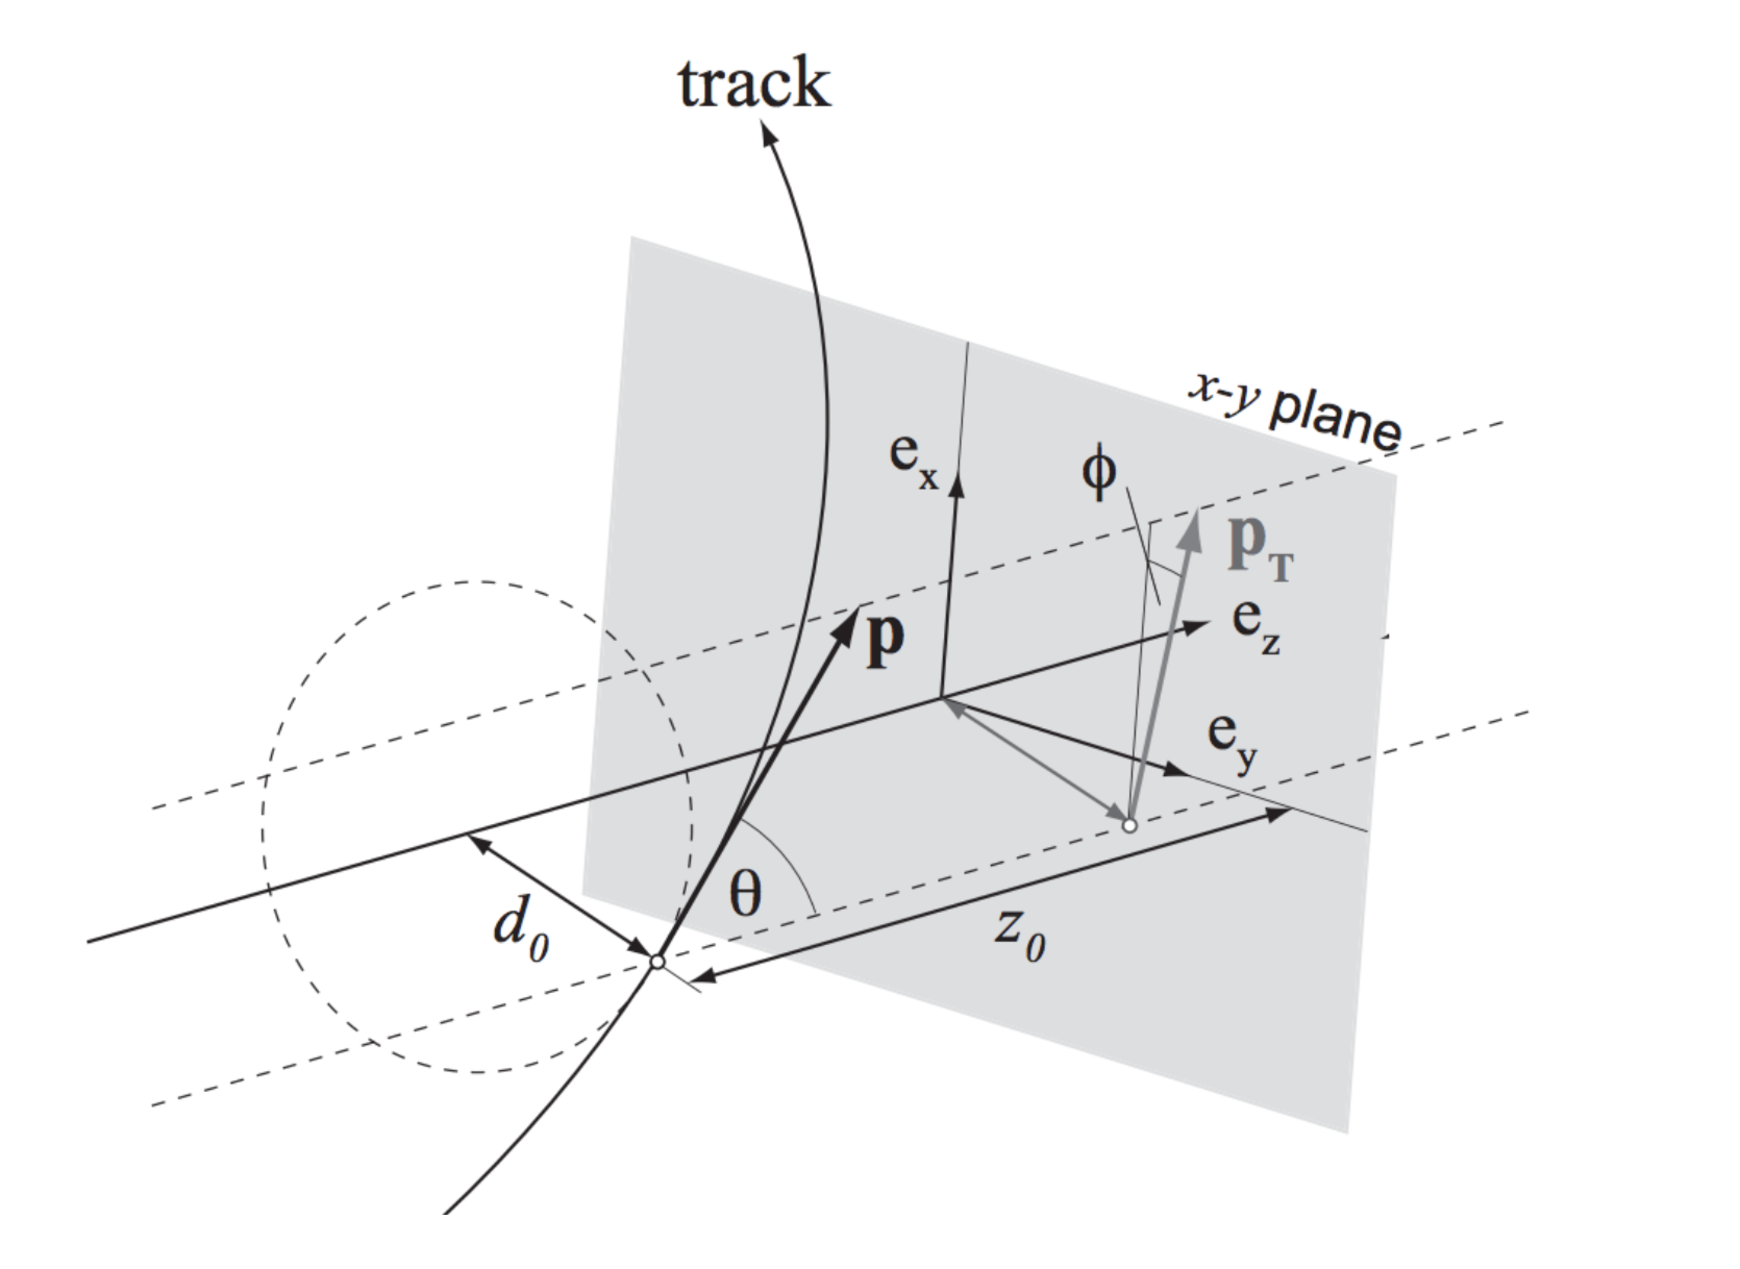
\includegraphics[width=0.60\textwidth]{figures/objects/track_param}
\caption{Schematic view of the track perigee parameters. Figure from Ref. \cite{Salzburger:track:perigee}.}
\label{fig:obj:tracks_param}
\end{figure}

Primary tracks, originating from charged particles with a life time longer that $3 \times 10^{-11}$ s produced directly in the hard-scatttering vertex, are reconstructed with an inside-out approach \cite{Cornelissen:1020106}: the seed of the reconstruction are three hits in the silicon detector, and then compatible hits in the outer layers of the \gls{id} are added with a Kalman Filter \cite{citeulike:347166,Fruhwirth:1987fm}. The \gls{trt} segments that are not associated with primary tracks are used as starting point to reconstruct tracks from long-lived particles or from material interaction, with a back-tracking that extrapolates the \gls{trt} information to the pixel hits. 

Random groups of hits can be wrongly reconstructed as belonging to the helical trajectory of a track (\textit{fake tracks}). The amount of fake tracks increases with the increase of pileup, and can be reduced by tightening the selection criteria of the track, at the expense of reconstruction efficiency. Three different selection criteria are used for the data collected in 2015 and 2016 (Loose, Loose-Primary and Tight-Primary), that differ in the requirements on the hits and holes (elements where a hit was expected but was not registered) in the different \gls{id} layers. The \textit{track reconstruction efficiency} is measured in \gls{mc} simulations as the ratio of the reconstructed tracks matched to a generated charged particle over the total number of generated charged particles. The reconstruction efficiency as a function of the track $\eta$ and \pt is shown in Figure \ref{fig:obj:tracks} for Loose and Tight-Primary tracks.
 
\begin{figure}[ht]
\centering
\subfigure[]{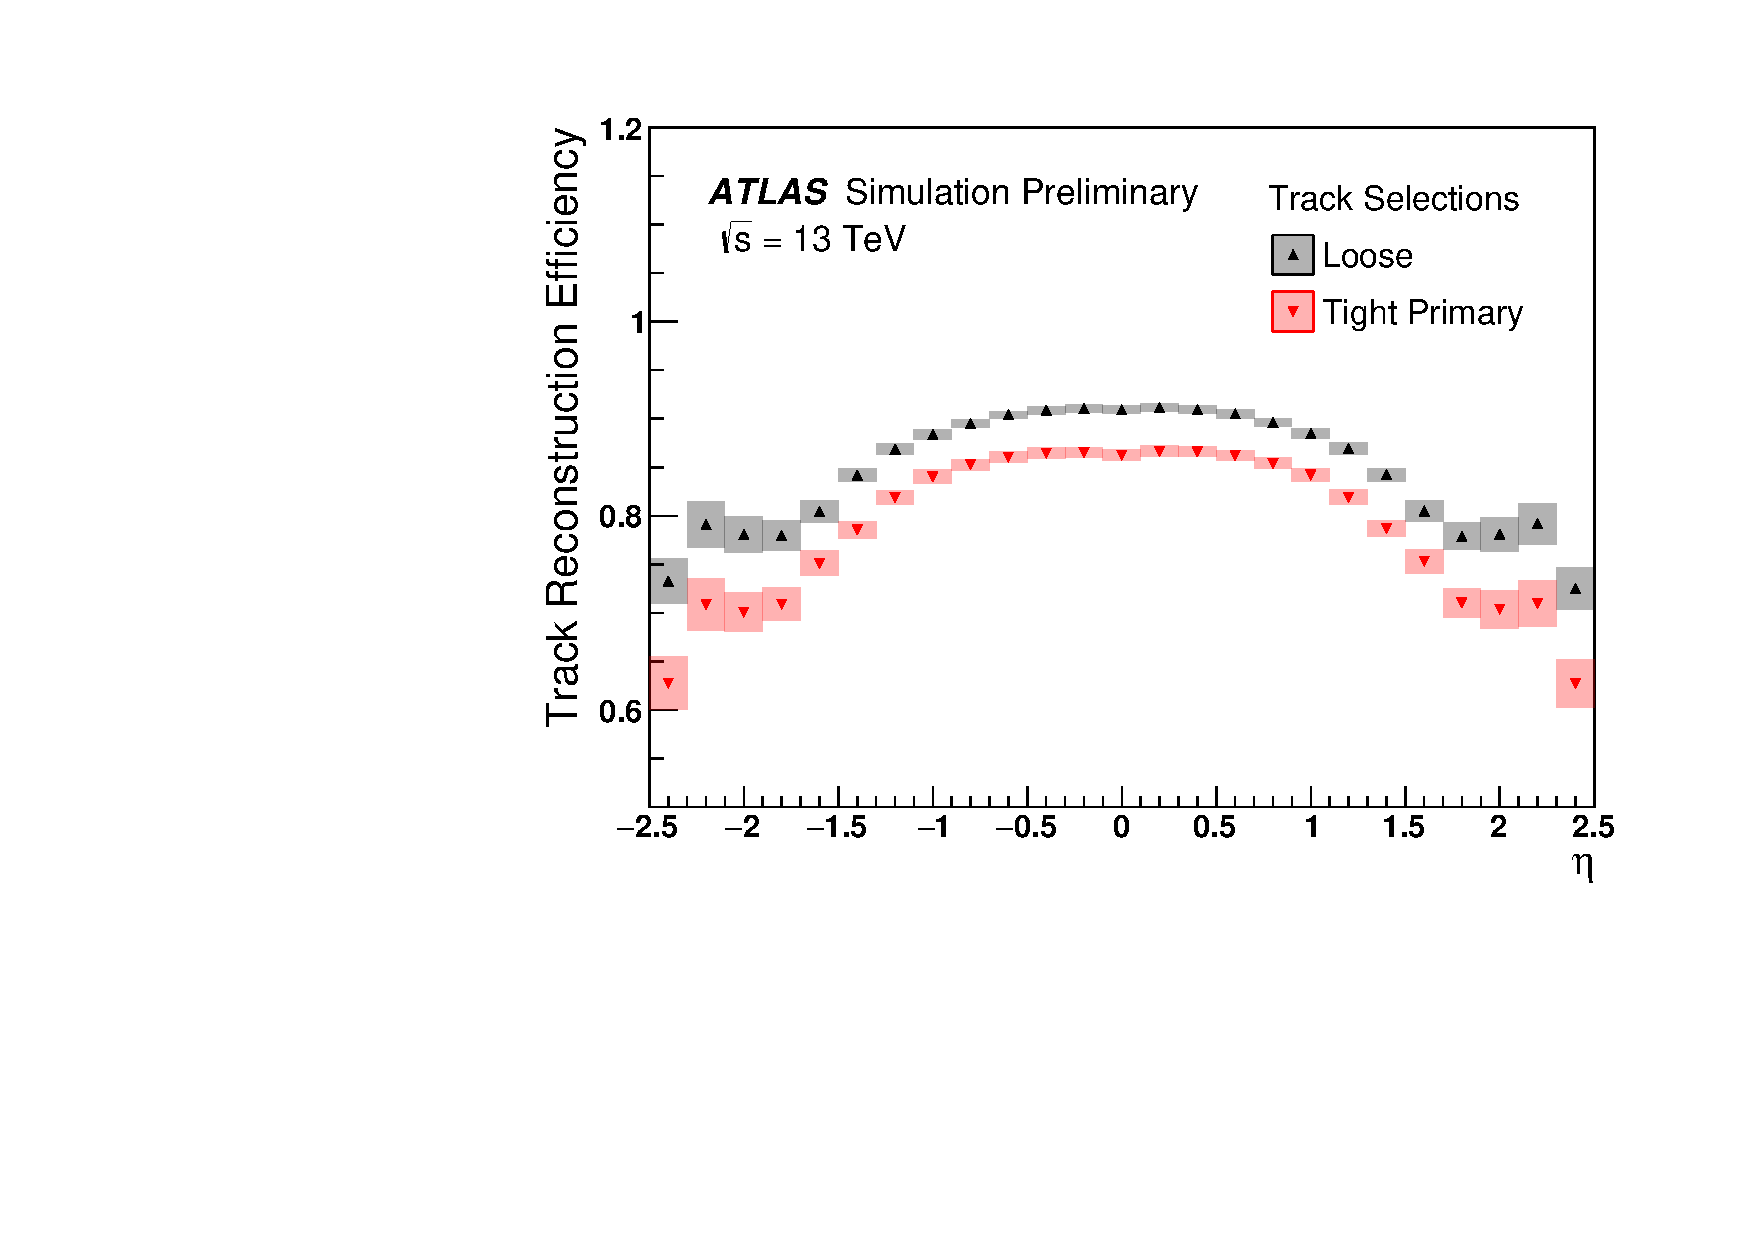
\includegraphics[width=0.48\textwidth]{figures/objects/track1}}
\subfigure[]{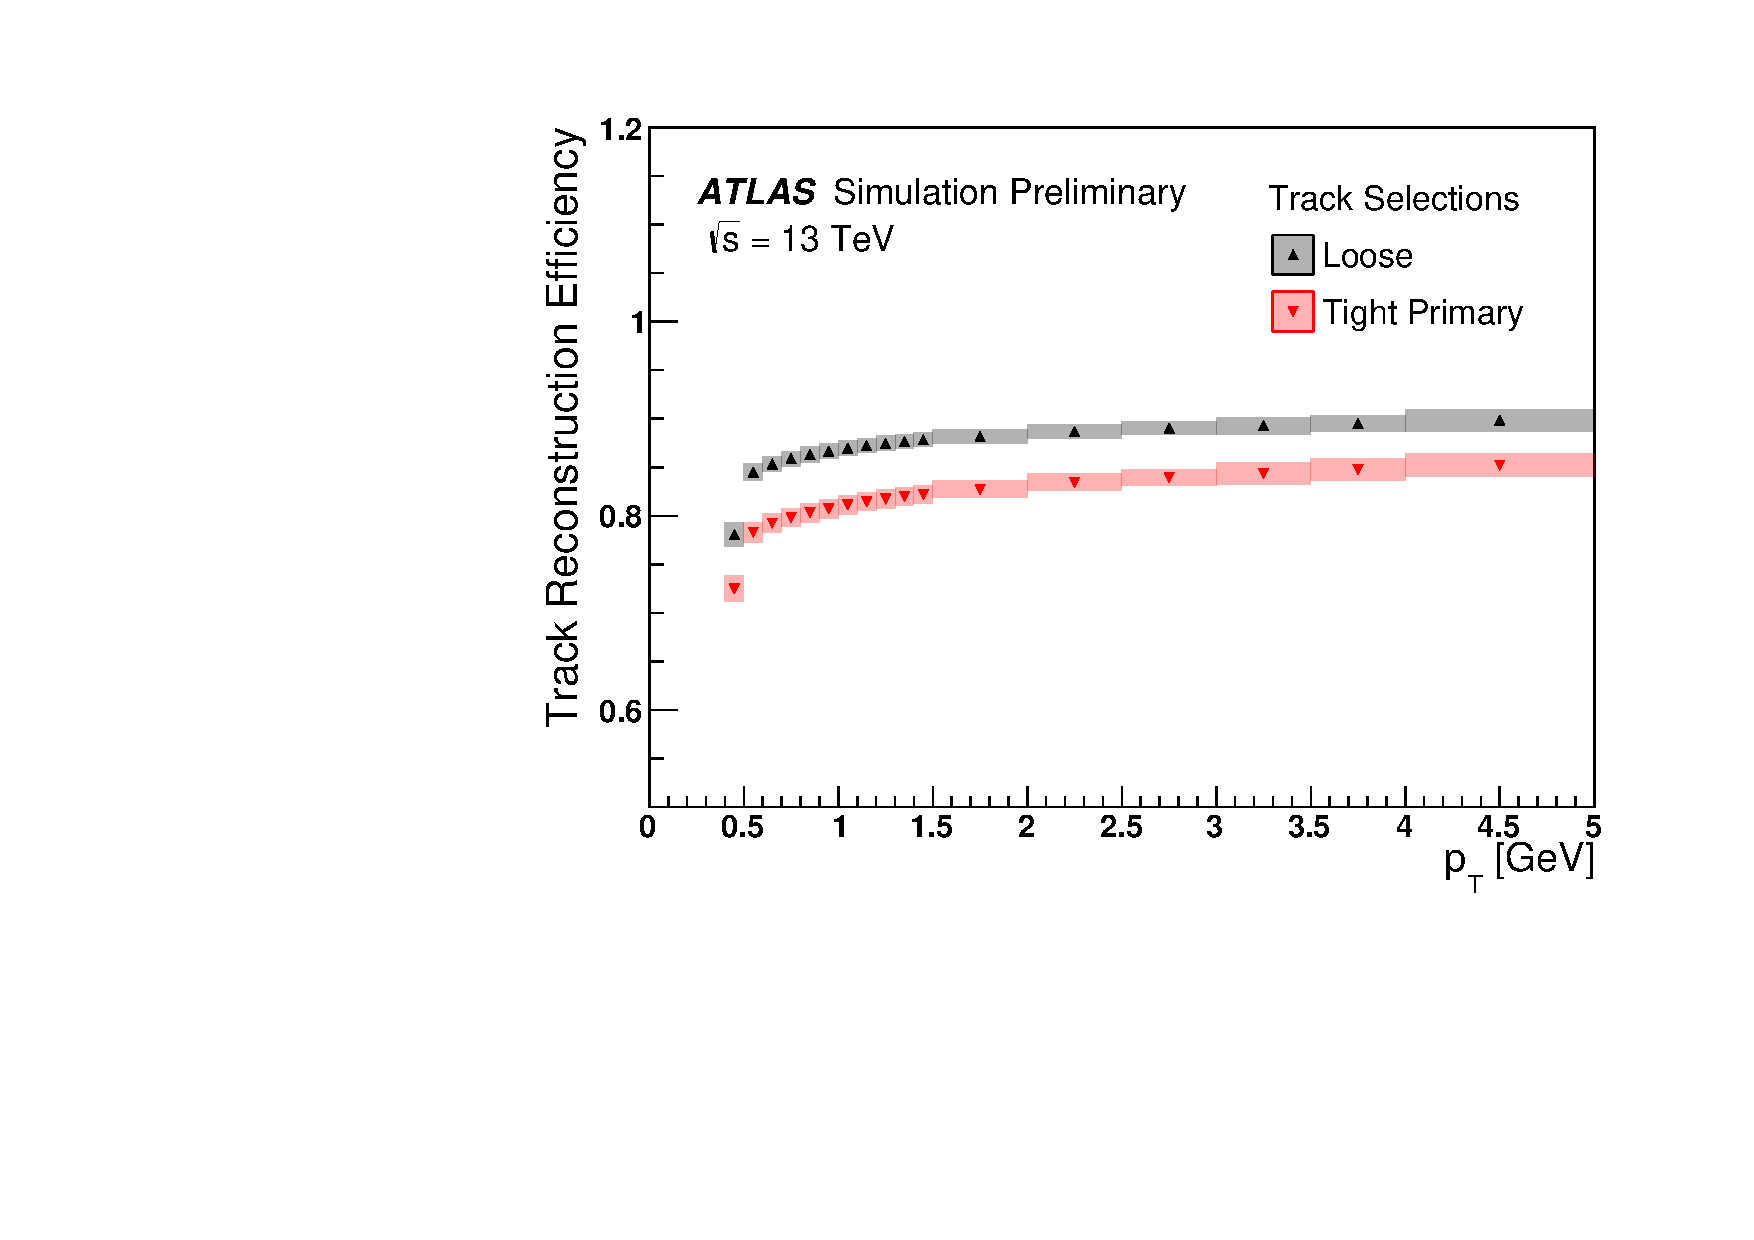
\includegraphics[width=0.48\textwidth]{figures/objects/track2}}
\caption{Track reconstruction efficiency, evaluated by using minimum bias simulated events, as a function of truth $\eta$ (a) and \pt (b) for Loose and Tight Primary track selections. The bands indicate the total sstematic uncertainty. Figure from Ref. \cite{ATL-PHYS-PUB-2015-051}.}
\label{fig:obj:tracks}
\end{figure}

Tracks are the starting point for the identification of the interaction points, referred to as \glspl{pv}. 
\glspl{pv} are reconstructed through a vertex finding algorithm \cite{Fruhwirth:2007hz}, 
and then the vertex fitting algorithm identifies the vertex position and refits the tracks 
adding the constraint of the reconstructed interaction point. 
The \gls{lhc} operates in a high-luminosity regime, which makes it likely to have multiple \gls{pp} interactions per bunch crossing, 
and therefore multiple reconstructed \gls{pv} candidates. 
Once all the \gls{pv} candidates are reconstructed, the one with the highest sum of the squared transverse momenta of its associated tracks ($\sum_i^{N-tracks}p_{T,i}^2$) is identified as the hard scattering \gls{pv}, and the position of physics objects is recomputed with respect to its coordinates. The other vertices are named pileup vertices, and their number is correlated  to the number of interactions per bunch crossing.


\section{Jets}

Because of confinement, quarks and gluons produced in the collisions give origin to a collimated spray of hadrons (\textit{jets}) that move in the direction of the original parton. When jets interact with the detector, they loose most of their energy as deposits in the calorimeter systems, which are then grouped together aiming at reconstructing the characteristics of the original parton. 

\subsection{Clusters}
The first step in the jet reconstruction is the procedure that groups the calorimeter cells in three dimensional objects referred to as topological clusters (\textit{topoclusters}) \cite{Lampl:2008zz,Aad:2016upy}. Topoclusters are built starting from seed cells with a signal-to-noise ratio higher than 4. All the neighboring cells with signal-to-noise ratio higher than two are added with an iterative procedure, and finally a ring of guard cells are added independently of their signal. This procedure is illustrated in Figure \ref{fig:obj:topocluster}. Topoclusters are calibrated at the \gls{em} scale, which means that the proportionality constant between the readout current and the particle energy is correct only for particles of an \gls{em} shower.

\begin{figure}[h]
\begin{center}
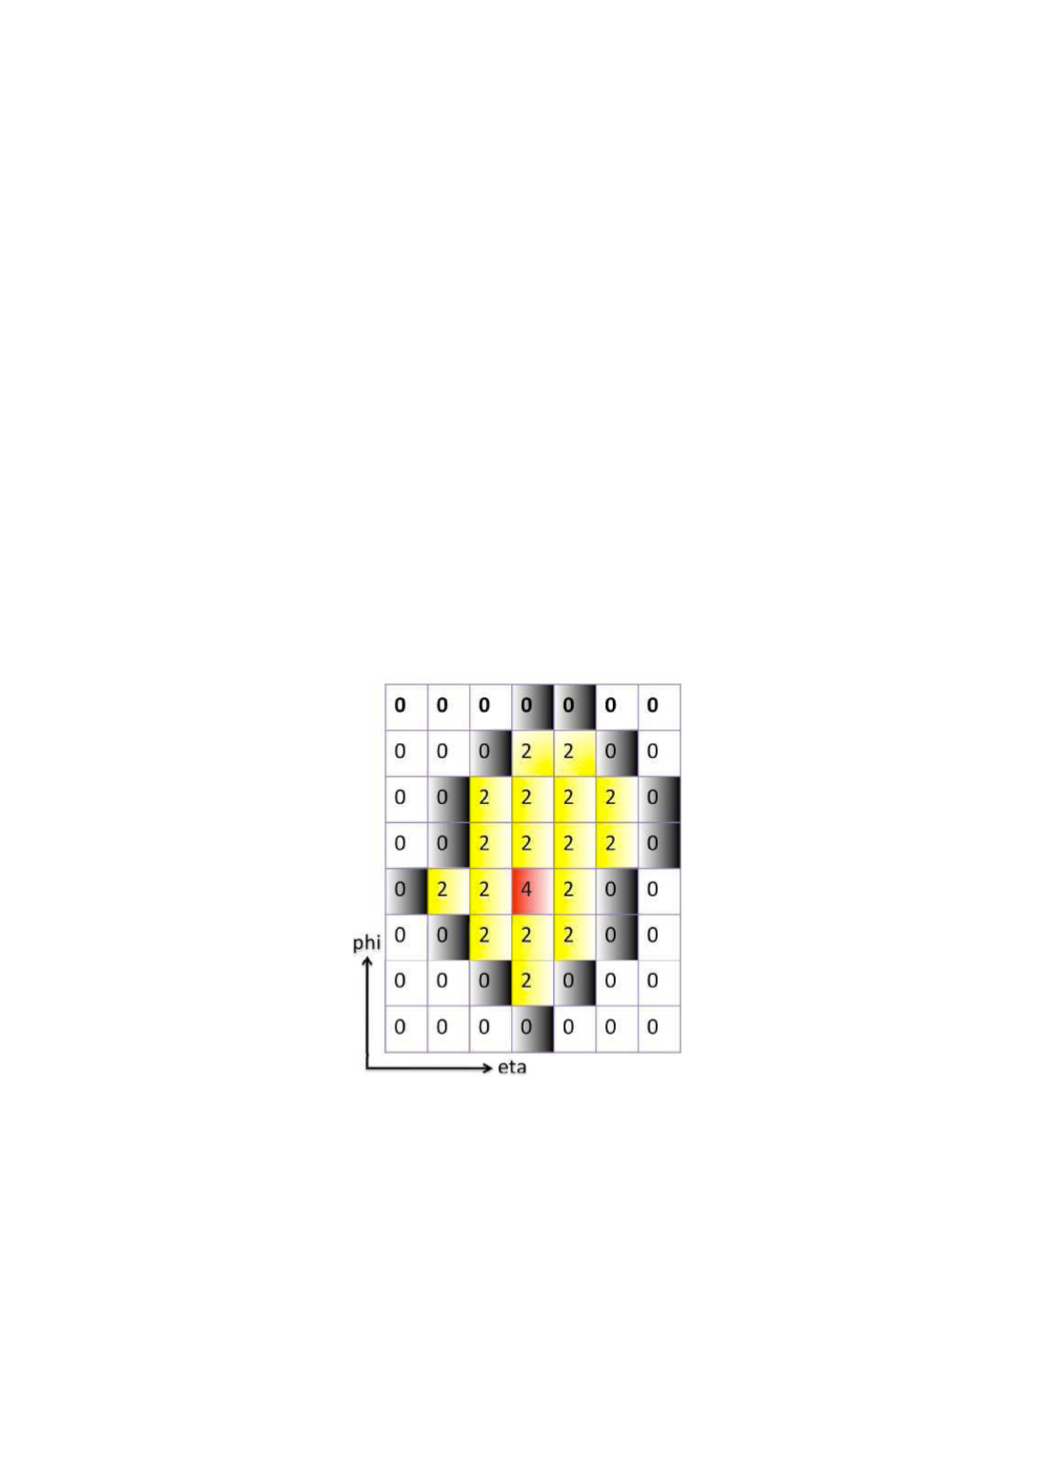
\includegraphics[width=0.3\textwidth]{./figures/objects/topocluster.pdf}
\end{center}
\caption[Topocluster schematic representation]{Topocluster schematic representation. The seed of the cluster is shown in red, the neighbouring cells are in yellow and the ring of guard cells is in grey.}
\label{fig:obj:topocluster}
\end{figure}
 
\subsection{Jet-finding algorithms}
\label{sec:obj:jetfinding}

The topoclusters are then grouped together by a jet-finding algorithm. Different algorithm are available, and in particular the algorithms of the $k_T$-family merge clusters according to the metric $d_{i,j}$, defined as:

\begin{equation}
d_{i,j} = min\left( k_{T,i}^{2n}, k_{T,i}^{2n}  \right) \frac{\Delta R_{i,j}^2}{R^2},
\label{eq:obj:dij}
\end{equation}

\noindent where $k_{T,i}$ is the transverse momentum of the cluster, $\Delta R_{i,j}$ is the angular distance defined as in \ref{eq:cern:dR}, 
$R$ is a fixed parameter, whose value sets the size of the jet, and $n$ is the parameters that defines the kind of algorithm we are using 
and therefore the shape of the resulting jets. 
Equation \ref{eq:obj:dij} defines the distance between two clusters, while the cluster-beam distance is defined as:

\begin{equation}
d_{i,B} =  k_{T,i}^{2n} \; .
\end{equation}

The grouping of clusters follows an iterative approach:
\begin{enumerate}
\item For each topocluster, the distances $d_{i,j}$ and $d_{i,B}$ are calculated.
\item If, for some $i$ and $j$, $d_{i,j} < d_{i,B}$, the two clusters with the smallest $d_{i,j}$ are grouped. 
\item Otherwise, if $d_{i,B} < d_{i,j} \, \forall i \neq j $ the $i$-th cluster is defined as a jet.
\item This procedure is iterated until all inputs have been classified into jets.
\end{enumerate}

\noindent Depending on the value of the parameter n, we can distinguish different algorithms:
\begin{itemize}
\item $n=0$: Cambridge-Aachen. The grouping of the clusters depends only on geometrical considerations and not on their momentum. 
\item $n=1$: $k_T$ algorithm. Soft clusters are grouped first.
\item $n=-1$: anti-$k_T$ algorithm. Groups hard objects first; the shape of the jets is more regular than in the two previous cases and is a cone of radius R.
\end{itemize}

The choice of a particular algorithm results in different shapes of the jets, represented in Figure \ref{fig:jetsalg}. The standard algorithm used by \gls{atlas} is the anti-$k_T$ algorithm \cite{cacciari:antikt}.

\begin{figure}[h]
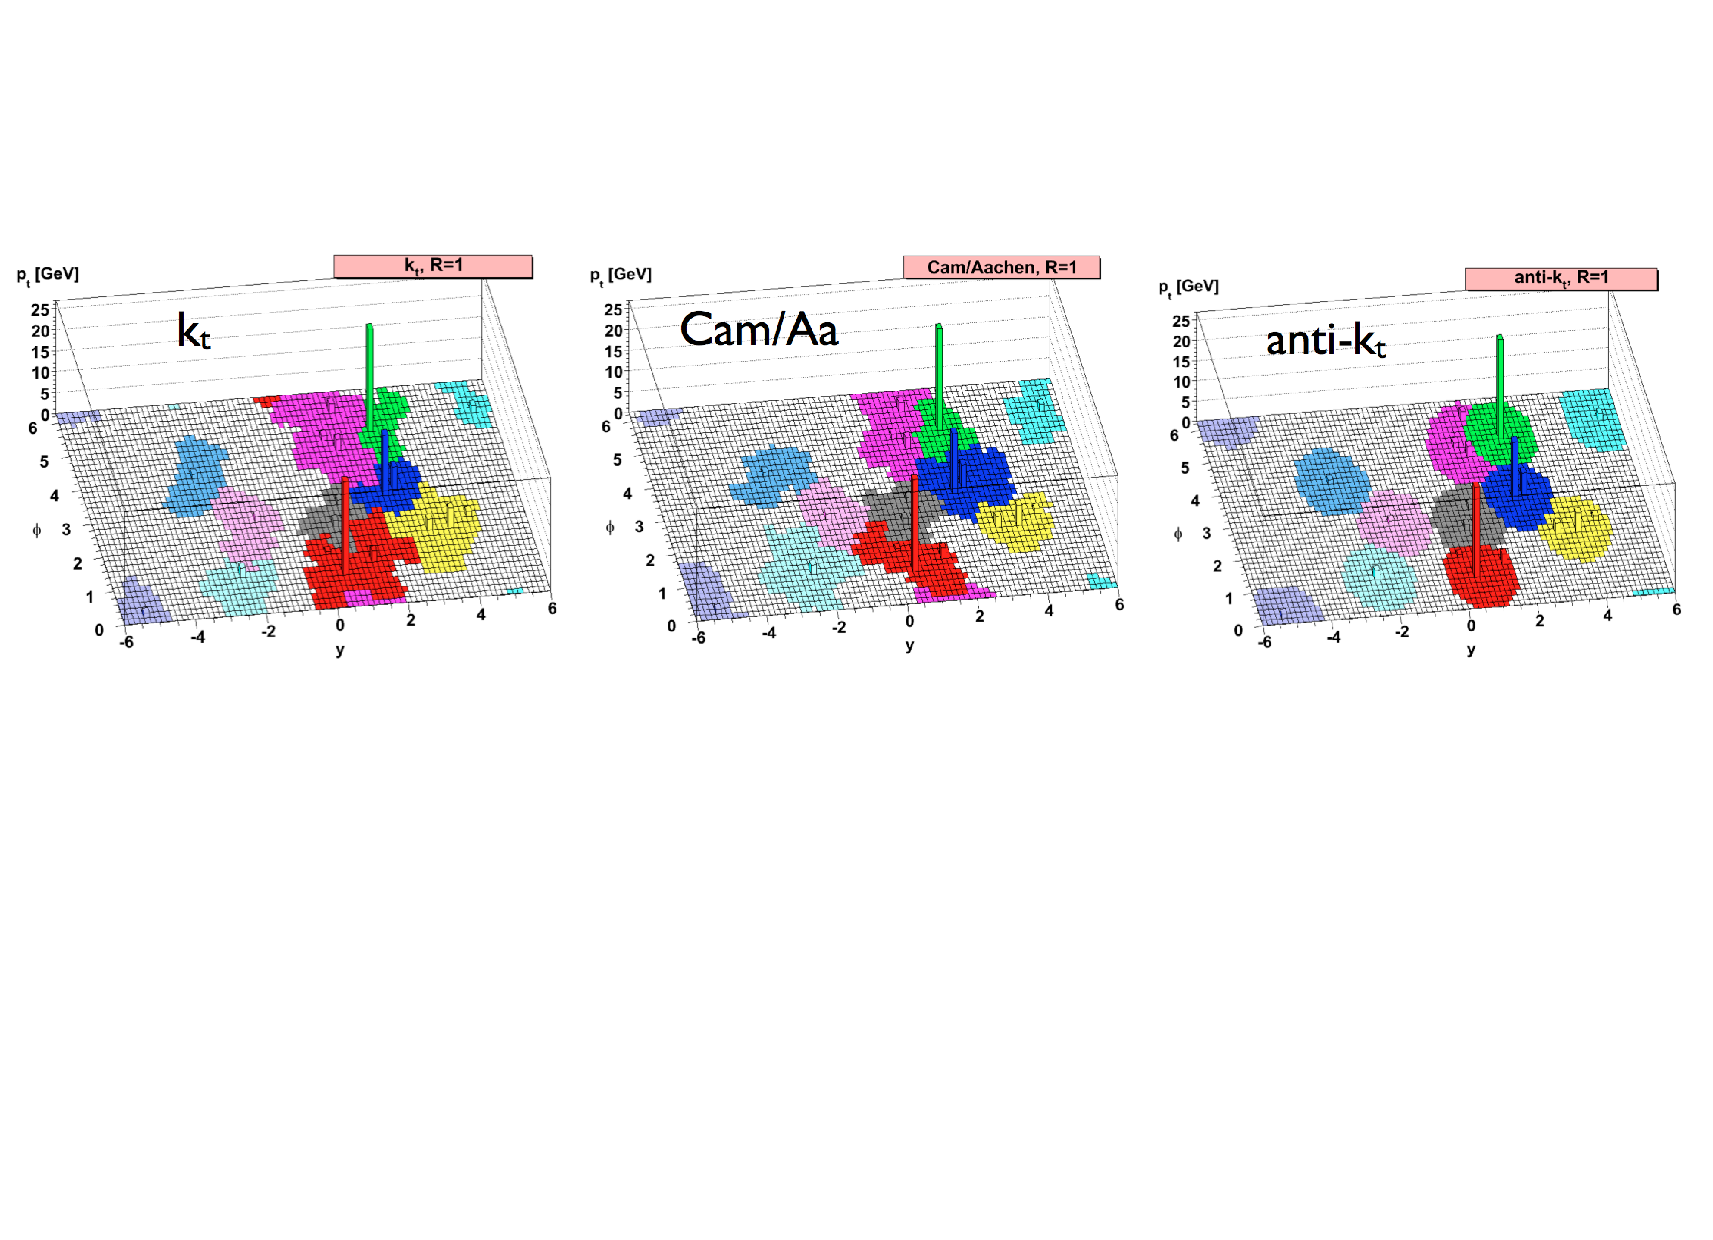
\includegraphics[width=\textwidth]{./figures/objects/jetsalg.pdf}
\caption[Shape of jets reconstructed with different algorithms]{Shape of jets reconstructed with different algorithms.
Figure from Ref. \cite{cacciari:antikt}.}
\label{fig:jetsalg}
\end{figure}

\subsection{Jet calibration}
\label{sec:obj:jetcalib}

As mentioned previously, the inputs to the jet-finding algorithm are calibrated at the \gls{em} scale, and its coordinates refer to the center of the detector. To access a more precise measurement of the jet energy and kinematics, a sequence of calibration steps is applied; 
%for the 2015-2016 dataset, 
the standard \gls{atlas} corrections are \cite{PhysRevD.96.072002}:

\begin{description}
\item[Origin correction] The direction of the jet is changed to point to the reconstructed hard-scattering \gls{pv} rather than to the cented of the detector. This correction improves the $\eta$ resolution of the jets.

\item[Pileup correction] Multiple collisions in the same bunch crossing (\textit{in-time pileup}), as well as residual energy from previous collisions (\textit{out-of-time pileup}), affect the jet energy reconstruction. The effect of pileup is corrected in two steps 
\cite{Cacciari:2007fd,TheATLAScollaboration:2013pia}: a first correction, dependent on the number of \glspl{pv}, uses the jet area to subtract form the jet energy the average energy form pileup events. 
The jet area is measured with ghost-association: simulated ghost particles of infinitesimal momentum are added to the event uniformly in solid angle prior to jet reconstruction, and the jet area is computed from the fraction of ghost particles associated to the jet after the clusters are merged. 
A second correction based on the number of \glspl{pv} and on the number of interactions per bunch crossing is then applied to disentangle the effect of in-time pileup and out-of-time pileup.

\item[Absolute calibration] The absolute \gls{jes} and $\eta$ correction is derived comparing in \gls{mc} the truth energy of a jet 
(defined as the energy of the truth jet with $\Delta R<0.3$ from the calorimeter jet) 
with the reconstructed energy, and it also corrects for biases in the $\eta$ reconstruction \cite{Aad2015jets}.

\item[Global sequential calibration] The \gls{gsc} \cite{ATLAS:2015oia} improves the \gls{jes} resolution by deriving additional corrections based on individual jet properties, e.g. the number of associated tracks and the fraction of energy deposited in the various layers of the calorimeter.

\item[In-situ calibration] As a last stage, the data-driven calibration (\textit{in-situ}) \cite{ATLAS:2015uwa} corrects for the differences between \gls{mc} simulation and data (arising e.g. from imperfect simulation of the detector response and material interaction). These corrections are derived from events where the jet \pt is balanced against other well measured objects. In the $\eta$-intercalibration, dijet events are used to correct the response of forward jets (with $0.8 < |\eta| < 4.5$) using well-measured central jets (with $|\eta| < 0.8$). 
The response of central jets is instead measured in $Z$+jets, $\gamma$+jets and multijet events; 
in $Z$/$\gamma$+jets events, the \pt of the jet is measured against the \pt of a well measured $Z$ boson or photon, while 
multijet events are used to calibrate central high-\pt jets ($300 < \pt < 2000$ GeV) against 
well calibrated low-\pt central jets. 
 
\end{description}

\subsubsection*{Jet calibration uncertainties}

The calibration procedure described above implies a set of uncertainties. In particular, 
the \gls{atlas} \gls{jes} Run-2 calibration includes a set of 80 systematic uncertainties; 
67 of those derive from the in-situ calibration \cite{PhysRevD.96.072002}, accounting for modelling uncertainties, 
sample statistics and uncertainties on the calibration of other physics objects used in deriving the calibration. 
The other 13 systematic uncertainties derive from the pileup correction, the $\eta$-intercalibration 
and differences in the jet response and composition for jets of different flavors. 
The full combination of the uncertainties derived from the first 3.2 \ifb of the Run 2 data 
is shown in Figure \ref{fig:obj:jessyst} as a function of \pt at $\eta = 0$ and as a function of $\eta$ at \pt$ = 80$ GeV.

\begin{figure}[h]
\begin{center}
  \subfigure[]{
    \label{fig:Comb_syst:pt}
    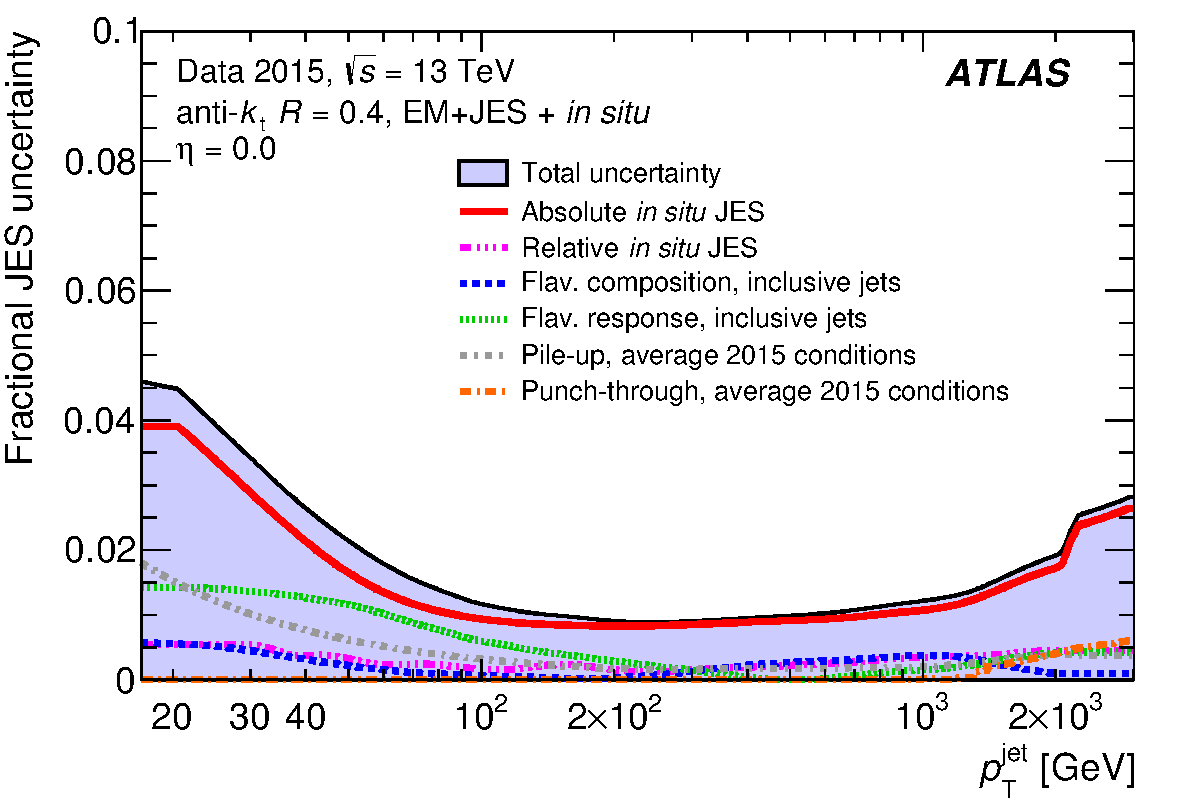
\includegraphics[width=0.48\textwidth]{figures/objects/fig12a.pdf}
  }
  \subfigure[]{
    \label{fig:Comb_syst:eta}
    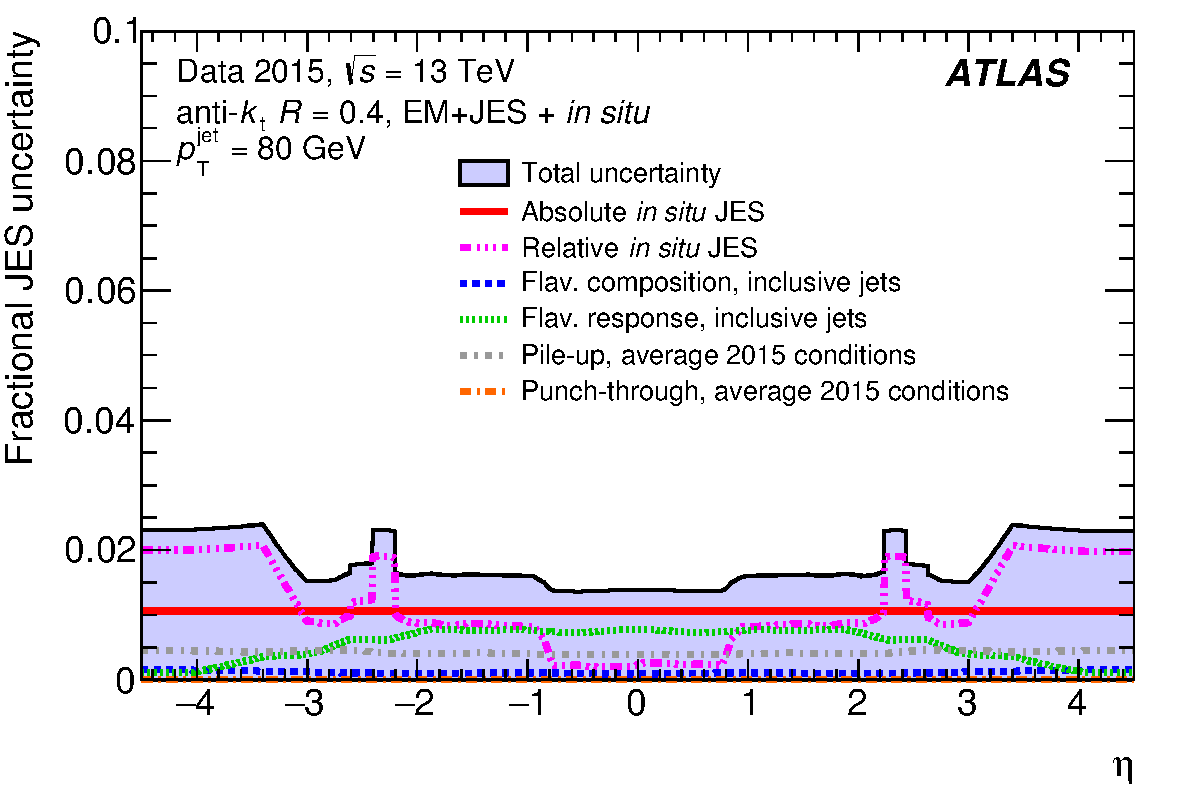
\includegraphics[width=0.48\textwidth]{figures/objects/fig12b.pdf}
  }
\end{center}
 \caption{Combined uncertainty in the \gls{jes} of fully calibrated jets as a function of \subref{fig:Comb_syst:pt}  
 jet \pt at $\eta = 0$ and \subref{fig:Comb_syst:eta} $\eta$ at \pt$ = 80$ GeV. Figure from Ref. \cite{PhysRevD.96.072002}.}
  \label{fig:obj:jessyst}
\end{figure}

To allow an easier usage of the uncertainties in physics analyses, a reduced set of 19 \gls{np} is provided: 
the 67 \glspl{np} from the in-situ calibration are reduced to six by keeping the five uncertainties of largest magnitude, 
plus a sixth one which is the sum in quadrature of the remaining ones. 
A further reduction is in place to group the remaining \glspl{np} into three components, 
and the \glspl{np} within a single component are added in quadrature; this leads to a correlation loss, whose effect is analysis dependent. 

Jets with the same true energy can have different reconstructed energies; the distribution of the difference between true and reconstructed energy of a jet is modeled with a Gaussian, whose width is defined as \gls{jer}. The measurements for the in-situ calibrations can be used also to access the differences in \gls{jer} between data and \gls{mc} \cite{TheATLAScollaboration:2015ofv,ATLAS:2015uwa}, and result into an additional \gls{np}.

\subsection{Jet Vertex Tagger}
\label{sec:jvt}

%It has already been discussed in Sec. \ref{sec:obj:jetcalib} how pileup is taken into account in the calibration of the \gls{jes}. 
Beside affecting the jet energy, high levels of pileup can also lead to the reconstruction of spurious jets not originating from the hard-scattering interaction. In \gls{atlas} track-based algorithms are used for the identification of pileup jets \cite{Aad:2015ina,ATLAS:2014cva}. 
Tracks are matched to calorimeter jets by ghost-association \cite{Soyez:2012hv}. Once the hard-scattering \gls{pv} (\gls{pv}$_0$) is identified, 
for each jet it is possible to compute the \gls{jvf}, the ratio of the scalar sum of the \pt of the tracks associated to the jet and originating from  \gls{pv}$_0$ to that of all the associated tracks:

\begin{equation}
 \JVF = \frac{\sum_m{p_{{\rm T}, m}^{{\rm track}}({\rm PV}_0)}}{\sum_n\sum_l  p_{{\rm T}, l}^{{\rm track}}({\rm PV}_n)} \; .
 \label{eq:jvf}
\end{equation} 

\noindent In this definition the index $n$ runs over all the vertices of the event. In high-pileup conditions the denominator in 
Equation \ref{eq:jvf} increases; to correct for this dependence, the \gls{cjvf} is introduced. 
This is a modified version of \gls{jvf}, that takes into account the dependence on the number of pileup tracks (\nPUtrk):

\begin{equation}
\cJVF = \frac{\sum_m{p_{{\rm T}, m}^{{\rm track}}({\rm PV}_0)}}{\sum_l p_{{\rm T}, l}^{{\rm track}}({\rm PV}_0) + \frac{\sum_{n\geq1}\sum_l p_{{\rm T}, l}^{{\rm track}}({\rm PV}_n)}{ (k \cdot \nPUtrk)}} \; ,
\label{eq:corrJVF}
\end{equation}

\noindent with $k=0.001$. Another variable used to discriminate hard-scattering jets against pileup jets is the ratio of the scalar
sum of the \pt of the tracks originating from \gls{pv}$_0$ to the jet transverse momentum:


\begin{equation}
\RpT = \frac{\sum_k{p_{\rm{T}, k}^{{\rm track}}({\rm PV}_0)}}{\ptjet} \;.
\label{eq:obj:rpt}
\end{equation}

The \cJVF and \RpT variables are combined in a two-dimensional likelihood that constitutes a single tagger, the \gls{jvt}. 
The distribution of \gls{jvt} for hard-scattering and pileup jets in \gls{mc} simulation is shown in Figure \ref{fig:obj:jvt_mc},
while Figure \ref{fig:obj:jvt_data} shows the comparison of the \gls{jvt} distribution in data and \gls{mc} in a di-muon selection.


\begin{figure}[h]
\begin{center}
  \subfigure[]{
    \label{fig:obj:jvt_mc}
    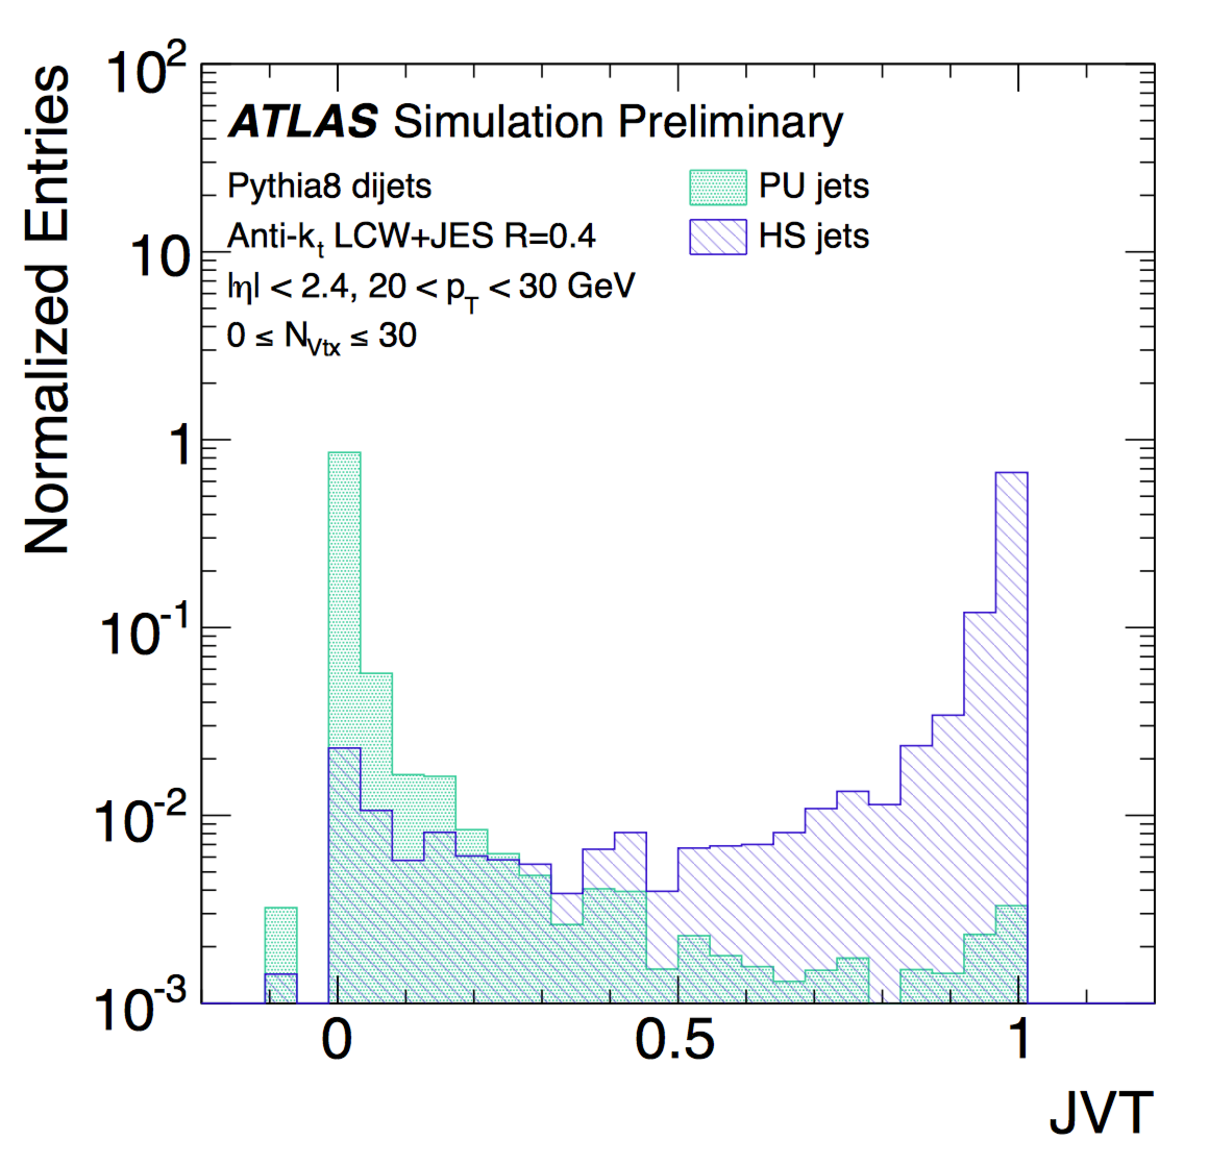
\includegraphics[width=0.43\textwidth]{figures/objects/jvt.pdf}
  }
  \subfigure[]{
    \label{fig:obj:jvt_data}
    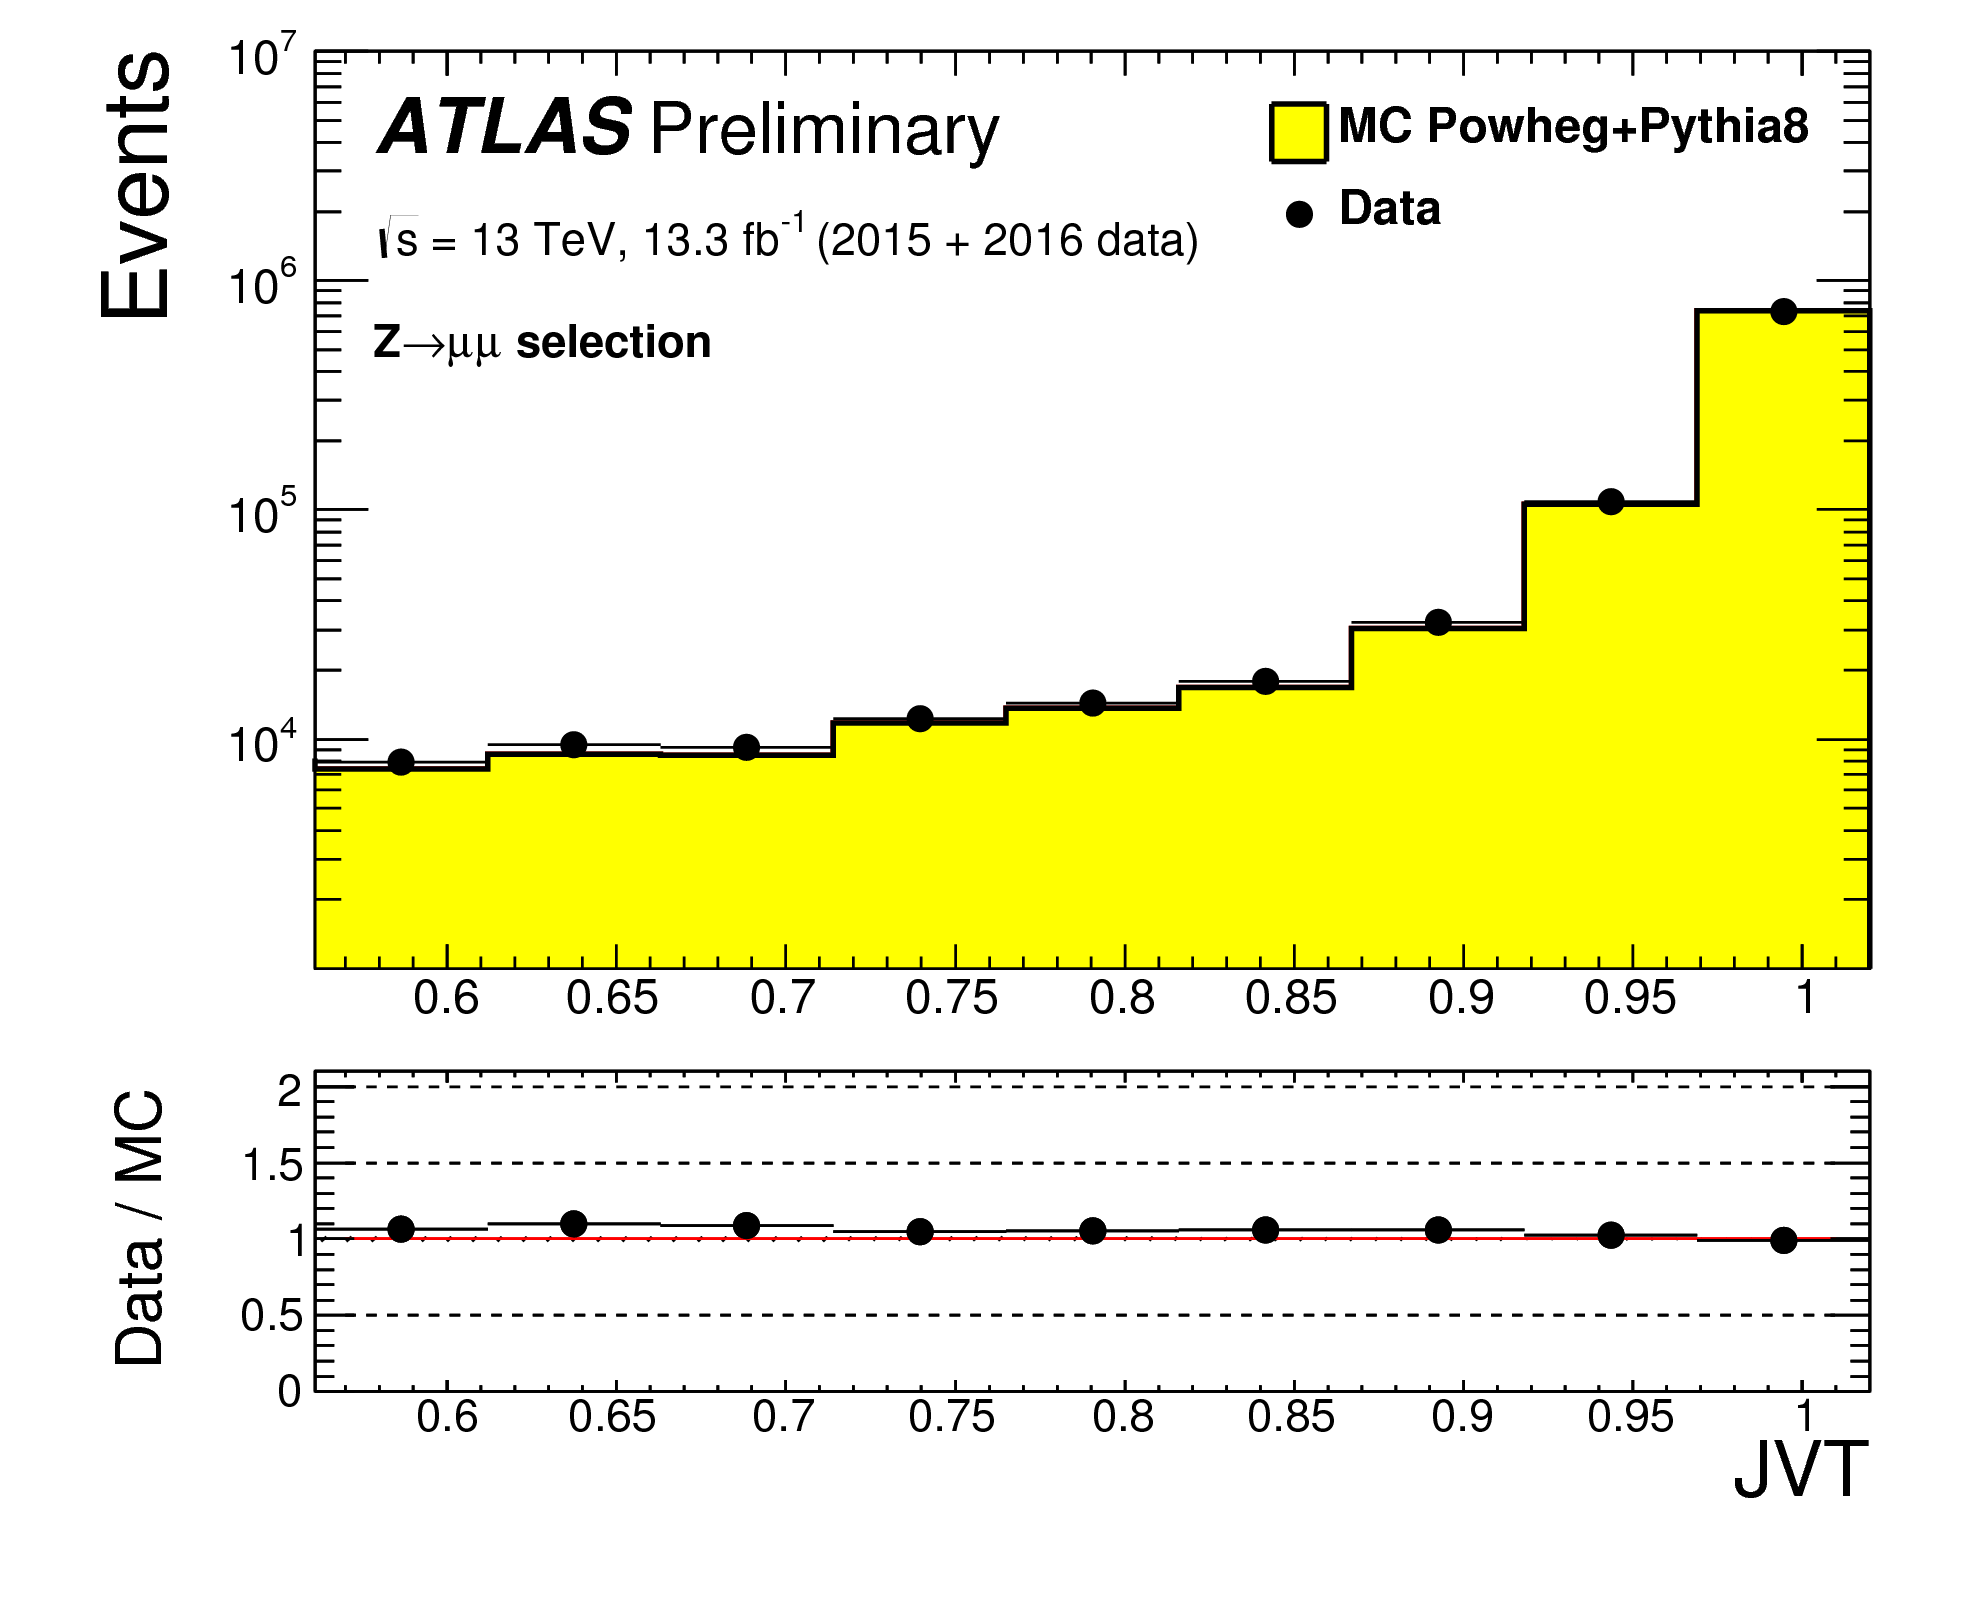
\includegraphics[width=0.53\textwidth]{figures/objects/jvt_data.png}
  }
\end{center}
 \caption{\subref{fig:obj:jvt_mc} Distribution of JVT for pileup and hard-scatter jets with $20 < \pt < 30$ GeV. Figure from Ref. \cite{ATLAS:2014cva}. \subref{fig:obj:jvt_data} The JVT distribution, in Powheg+Pythia8 MC and in 2015+2016 data, of jets balanced against Z bosons decaying to muons. Figure from Ref. \cite{jvtpublicplots}.}
  \label{fig:obj:jvt}
\end{figure}

\subsection{Jet cleaning}
\label{sec:jetcleaning}

Beside pileup jets, other spurious jets come from the non-collision background; this type of background includes muons originating from secondary cascades from beam losses, in which case we speak of beam-induced background, and from cosmic rays. These muons leave energy deposits in the calorimeters while traversing the detector, which can be interpreted as jets. Also coherent noise from the calorimeters can give rise to fake jets. In \gls{atlas} a set of quality criteria are designed to reject jets not originating from \gls{pp} collisions \cite{TheATLAScollaboration:2015ofz}. These quality criteria are rely on variables based on:
\begin{itemize}
\item Ionization signal shape in the LAr calorimeters, to remove mainly fake jets from calorimeter noise. 
\item Ratios of energies, e.g. the ratio of the energy deposited in the electromagnetic calorimeter to the total energy, or the ratio of energy in different calorimeter layers, that can be used to discriminate against jets from beam-induced background or calorimeter noise.
\item Tracks associated with the jets, and in particular variables similar to \RpT defined in Equation \ref{eq:obj:rpt}, that have in general lower value for fake jets than for jets originating from \gls{pp} collisions. 
\end{itemize} 

Different thresholds for the selections on these variable distinguish the two working points, \textit{BadLoose} and \textit{BadTight}, which have an efficiency respectively of 99.5\% and 95\% for jets with $\pt > 20$ GeV, while for jets with $\pt > 100$ GeV the efficiency of the two working points increases to 99.9\% and 99.5\%. The \gls{op} used in the searches discussed in Chapters \ref{chap:strong_prod} and \ref{chap:ewk_prod} is \textit{BadLoose}. 

\subsection{Re-clustered jets}
\label{sec:reclustering}

The angular separation between the decay products of a particle with mass $m$ and transverse momentum 
$p_T$ scales as:
\begin{equation}
\Delta R \approx \frac{2 m}{p_T} \; .
\end{equation}

This indicates that the ideal value of the $R$ parameter described in Sec. \ref{sec:obj:jetfinding} can vary depending on the event topology that we want to capture. 
For example, the decay products of a heavy particle with a transverse momentum much larger than its rest mass (\textit{boosted object}) could be better described by a 
single jet with a larger $R$ than with multiple jets with the "standard" 0.4 radius, 
as it happens e.g. in the decay of very energetic top quarks, $W$, $Z$ or Higgs bosons produced at the LHC.
Each different value of the $R$ parameter requires a dedicated calibration following the steps described in Sec. \ref{sec:obj:jetcalib}. 
Therefore, it is not always possible to choose the optimal value of the jet radius. 
A possible solution to this problem comes from noticing that the same jet-finding algorithms used to group topoclusters can have different types of inputs. 
In particular, jets themselves can be be used as input and grouped together, and in this case we speak of \textit{re-clustered jets} \cite{Nachman:2014kla}. 
Re-clustered jets are automatically calibrated as long as the input jets are, and also the jet uncertainties can be propagated directly. 
A comparison of the jet clustering obtained with anti-$k_T$ $R$=1.0 and by re-clustering anti-$k_T$ $R$=0.3 jets into anti-$k_T$ $R$=1.0 jets 
is shown in Figure \ref{fig:recluster}. It is possible to see how the jet axis is similar between the two cases, and how the anti-$k_T$ $R$=1.0 jets have more inputs away from the jet axis.
Re-clustered jets can be \textit{trimmed} by removing the constituent small-R jets that have a \pt smaller than a defined fraction of the \pt of the original reclustered jet. 


\begin{figure}[h]
\begin{center}
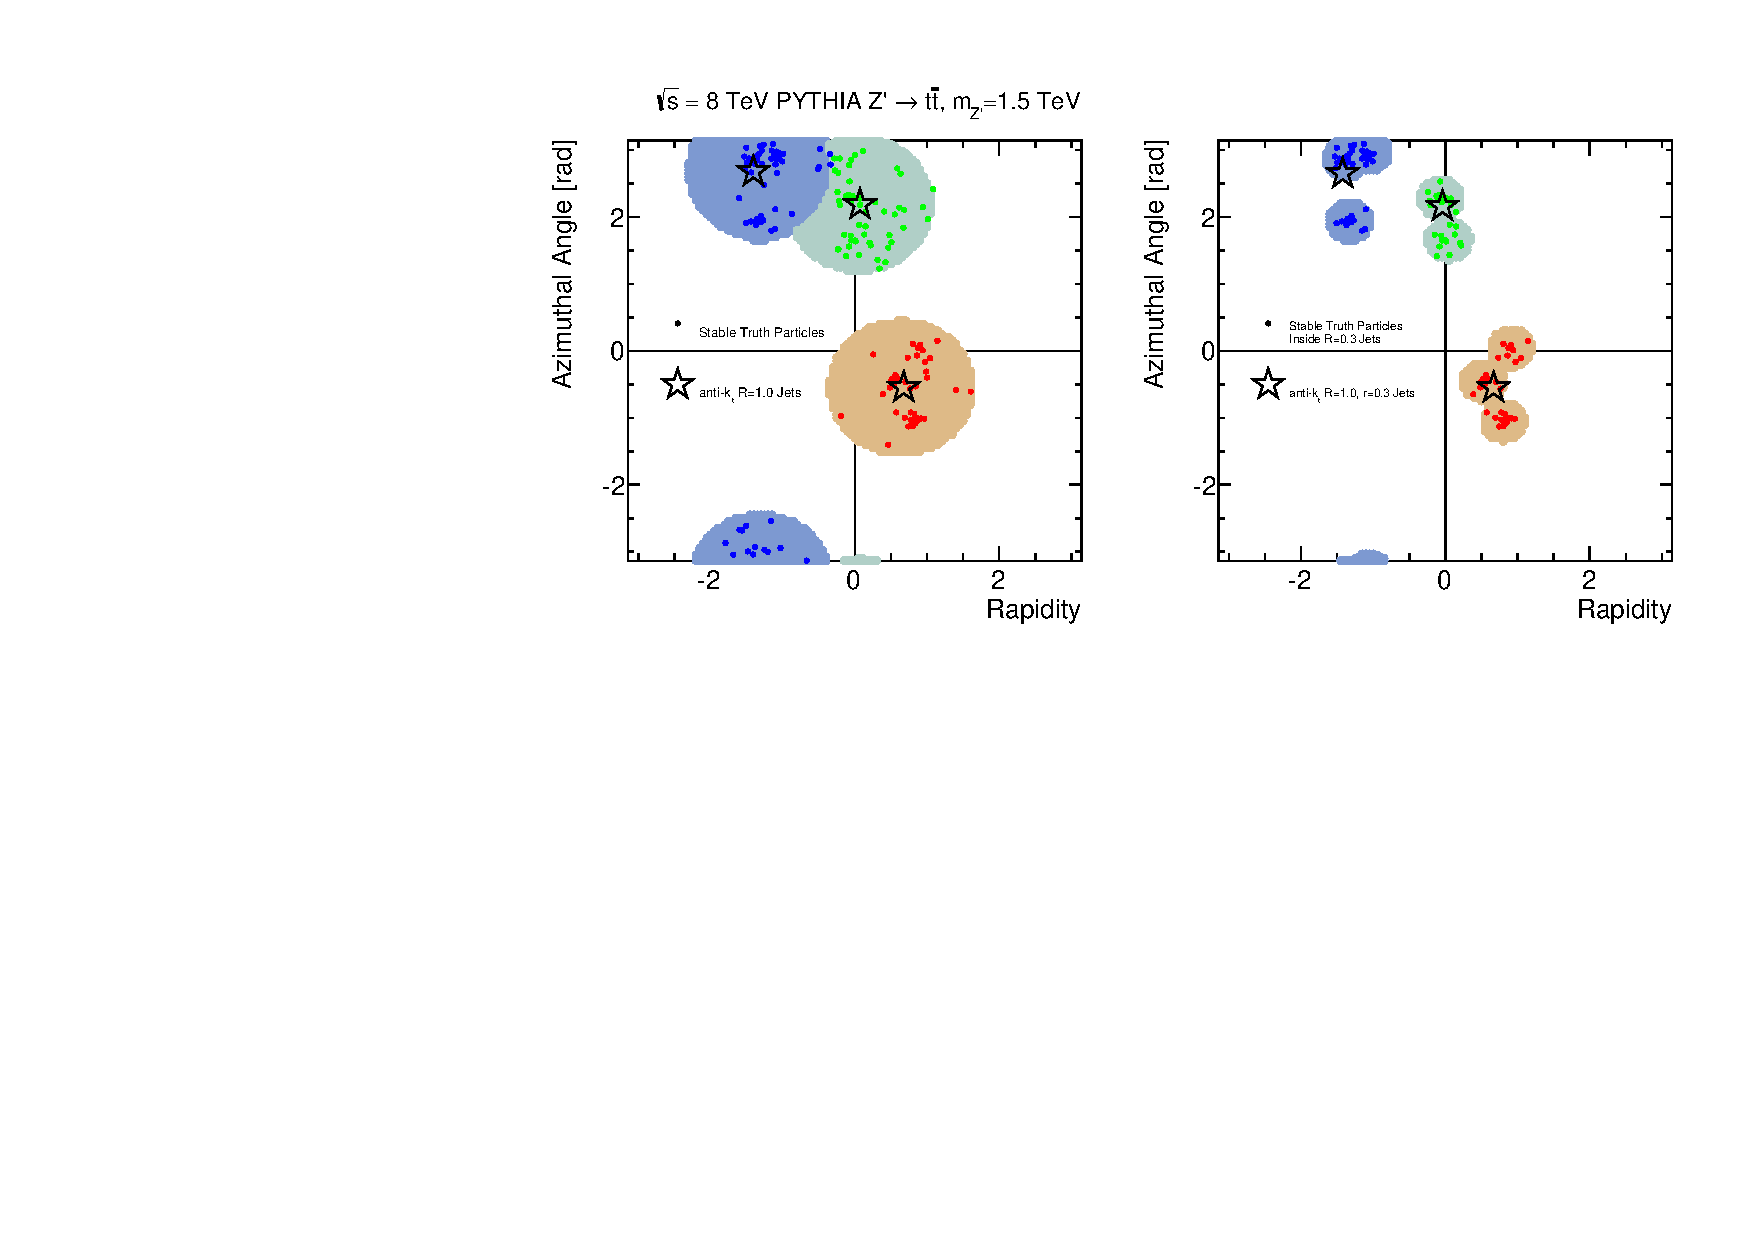
\includegraphics[width=1.0\textwidth]{./figures/objects/reclustered.pdf}
\end{center}
\caption{Example event where jets have been clustered with (a) anti-$k_T$ with $R$=1.0 and (b) anti-$k_T$ $R$=1.0 re-clustered jets (starting from anti-$k_T$ $R$=0.3 jets); the shaded region shows the jet area. Figure from Ref. \cite{Nachman:2014kla}.}
\label{fig:recluster}
\end{figure}

\section{Jets from B-hadrons}
\label{sec:btagging}

Jets originating from the hadronization of a $b$-quark (\textit{$b$-jets}) can be identified thanks to the lifetime of $B$-hadrons (about $10^{-12}$ s), which is shorter than the typical lifetime of hadrons containing only light quarks, but still long enough to allow the $B$-hadrons to travel distances of the order of the mm before decaying. A schematic view of the topology originating from a jet containing a $B$-hadron is shown in Figure \ref{fig:btag}. 
\begin{figure}[h]
\begin{center}
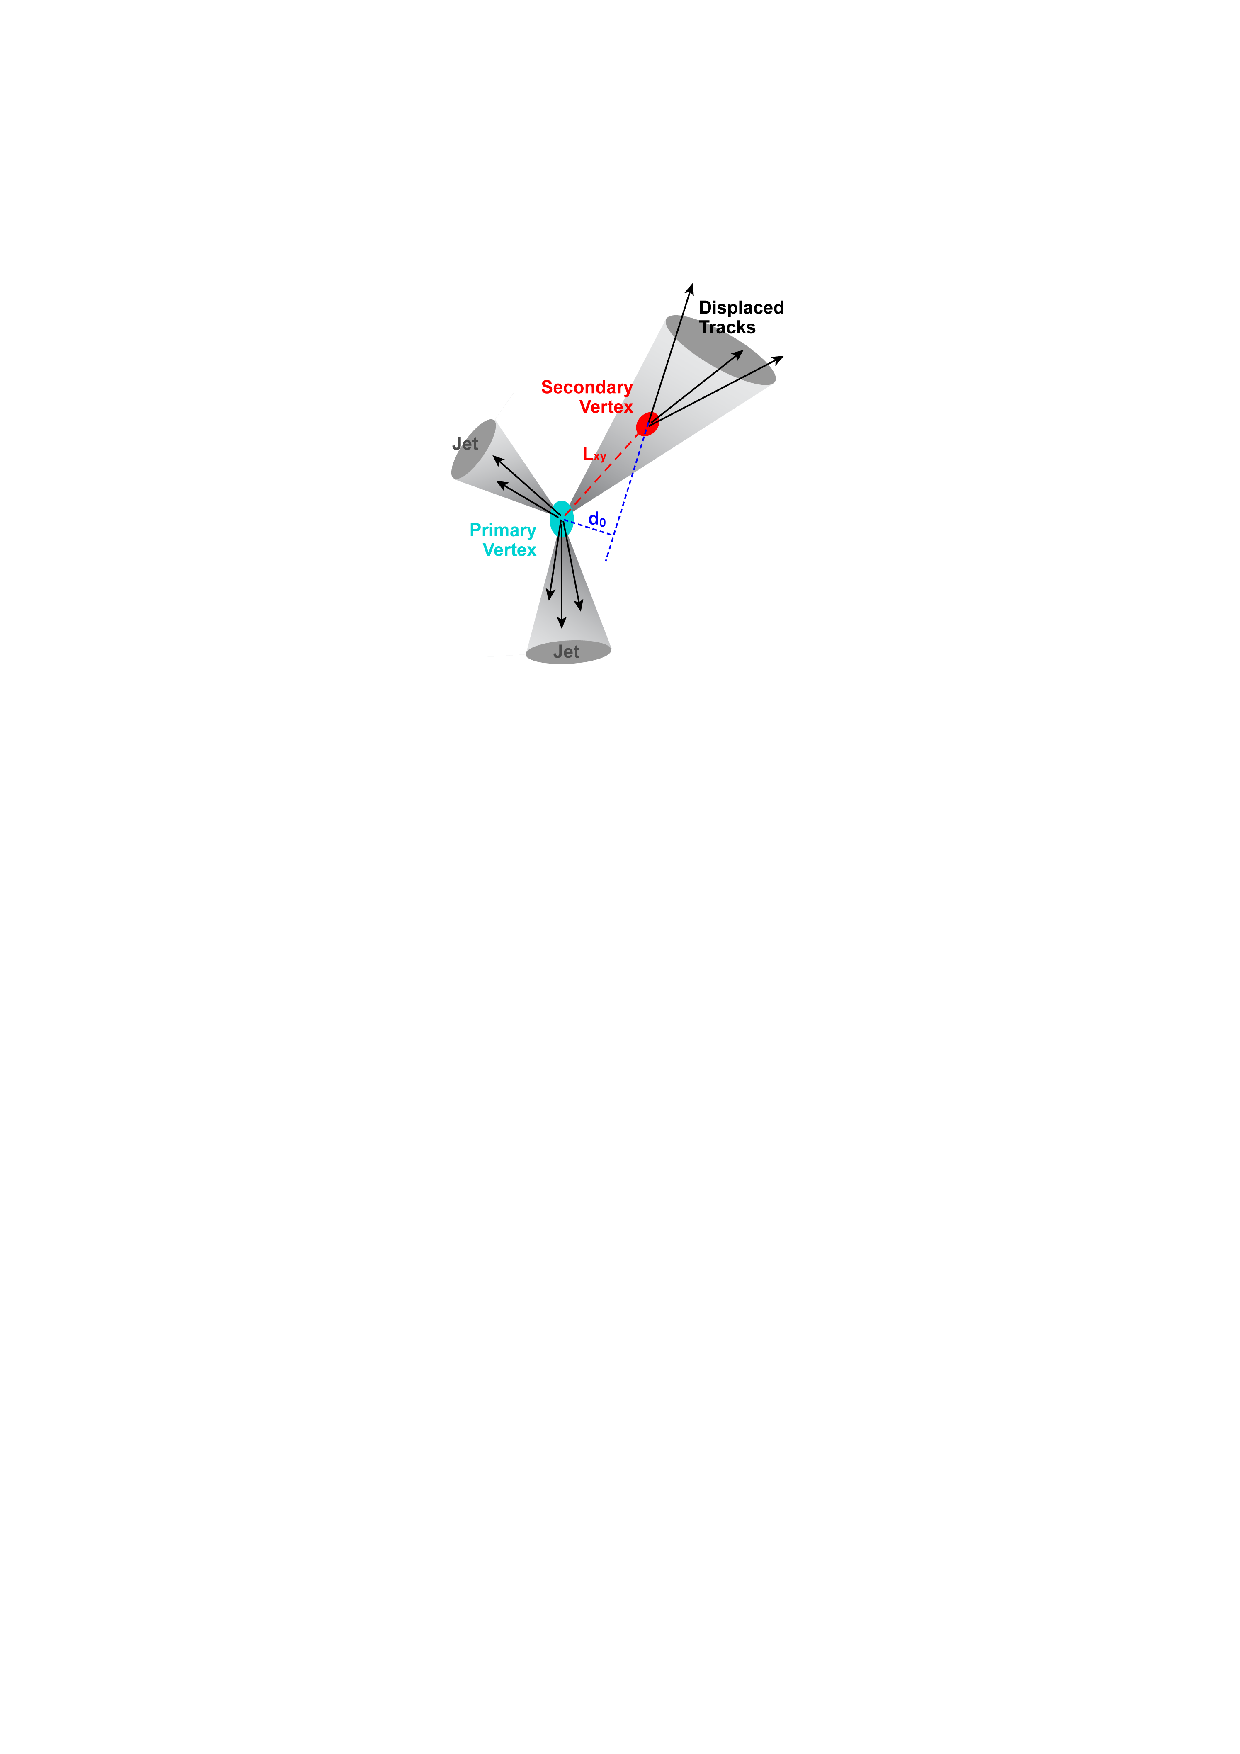
\includegraphics[width=0.45\textwidth]{./figures/objects/secvtx.pdf}
\end{center}
\caption[Schematic view of the topology of a $b$-jet.]{Schematic view of the topology of a $b$-jet. Figure from Ref. \cite{d0btagging}.}
\label{fig:btag}
\end{figure}
The procedure of identifying $b$-jets is referred to as \textit{$b$-tagging}, and in \gls{atlas} is performed using as input the tracks associated to the jets . As already mentioned in Sec. \ref{sec:atlas:pixel}, between Run 1 and Run 2 a fourth pixel layer, the \gls{ibl}, was added to the \gls{atlas} detector, allowing a better impact parameter resolution and therefore improving substantially the $b$-tagging performance. 

There are three families of $b$-tagging algorithms that can be combined through multivariate techniques. The basic algorithms can be based on:

\begin{description}

\item[Impact Parameter] The transverse impact parameter of a track (\dzero) is the point of closest approach to the 
\gls{pv} in the transverse plane, while the longitudinal impact parameter (\zzerost) is defined as the distance along 
the $z$-axis between the \gls{pv} and the point of closest approach in the transverse plane. Because of the typical 
lifetime of $B$-hadrons, on average $b$-jets contain tracks with higher impact parameter than light-jets. 
The sign of the impact parameter is positive if the track extrapolation crosses the jet direction in front of the primary vertex, and negative otherwise. 
The negative side of the impact-parameter distribution derives from the 
impact-parameter resolution, and can be used to calibrate light-jets. In \gls{atlas}, two taggers make use of the information on the impact parameter
 \cite{ATLAS:2011qia}: IP2D, which is based on the significance of the transverse impact parameter (\dzero/$\sigma_{\dzero}$), and IP3D, which builds a two-dimensional template including also the significance of the longitudinal impact parameter (\zzerost/$\sigma_{\zzerost}$). The \gls{pdf} for each flavor hypothesis ($b$, $c$, and light) is derived from \gls{mc} simulation on a per-track basis, and then a \gls{llr} of the different probabilities is computed, including the contribution from all tracks associated to the jet. For example, the \gls{llr} discriminating $b$-jets from light-jets is of the form $\sum_{i=1}^{N}\log\frac{p_b}{p_{light}}$, where the index $N$ runs on all the tracks associated to the jet. 

\item[Secondary Vertex Finding] The SV1 algorithm \cite{ATLAS:2011qia} explicitly looks for a secondary vertex within a jet. 
All the track pairs in the jet are tested for a two-track vertex hypothesis, removing the pairs that are likely to originate from 
long-lived particles (e.g. K$_0$, $\Lambda$), photon conversion or hadronic interaction with the detector material. 
If a two-track vertex remains, a new single vertex is fitted with the tracks passing this selection. 
Jets that are $b$-tagged for high values of a likelihood discriminant, built using several variables 
including the decay-length signicance, the invariant mass of all tracks associated with the vertex, 
the ratio of the sum of the energies of the tracks in the vertex to the sum of the energies of all tracks in the jet, 
and the number of two-track vertices.

\item[Identification of the Decay Chain] The $B$-hadrons inside $b$-jets decay with an electroweak interaction, 
through which a $b$-quark decays preferentially into a $c$-quark, since the \gls{ckm} matrix element $|V_{cb}|^2$ is much larger than $|V_{ub}|^2$. Hadrons containing a $c$-quark ($D$-hadrons) subsequently decay as well, giving rise to a topology with two decay vertices. While the resolution is often not enough to reconstruct the two vertices individually, the JetFitter algorithm \cite{1742-6596-119-3-032032} operates assuming that they both lie on the same line, the flight axis of the $B$-hadron. The information on the event topology derived with JetFitter is then used in a likelihood function, from which three different templates (one for each flavor) are derived.

\end{description}

The default $b$-tagging algorithm used by \gls{atlas} in the analysis of the 2015-2016 dataset is MV2c10 
\cite{ATL-PHYS-PUB-2015-022,ATL-PHYS-PUB-2016-012}, 
a multivariate algorithm based on a \gls{bdt} that combines the algorithms described above. 
MV2c10 belongs to the family of MV2 algorithms, which are trained on a \ttbar sample using $b$-jets as signal and $c$-jets and light-jets as background, and differ in the relative fraction of $c$-jets and light-jets that are
used in the training; in the case of MV2c10, the background sample in the training contains 15\% of $c$-jets.
Figure \ref{fig:obj:mv2} shows the light-jet and $c$-jet rejection as a function of $b$-jet efficiency for different MV2 algorithms.

\begin{figure}[h]
\begin{center}
  \subfigure[]{
    \label{fig:obj:mv2_a}
    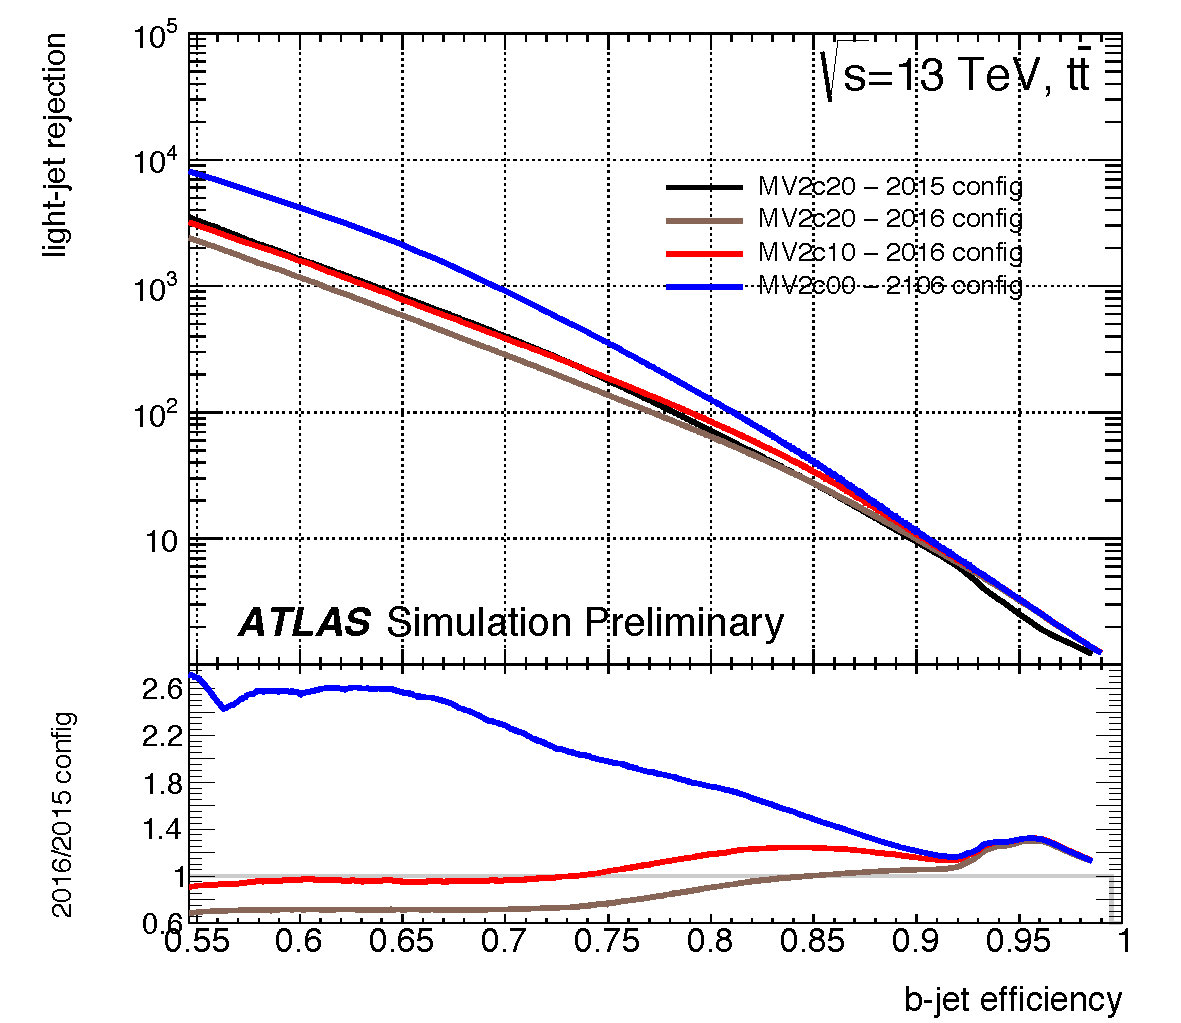
\includegraphics[width=0.48\textwidth]{figures/objects/mv2c10_a.pdf}  }
  \subfigure[]{
    \label{fig:obj:mv2_b}
    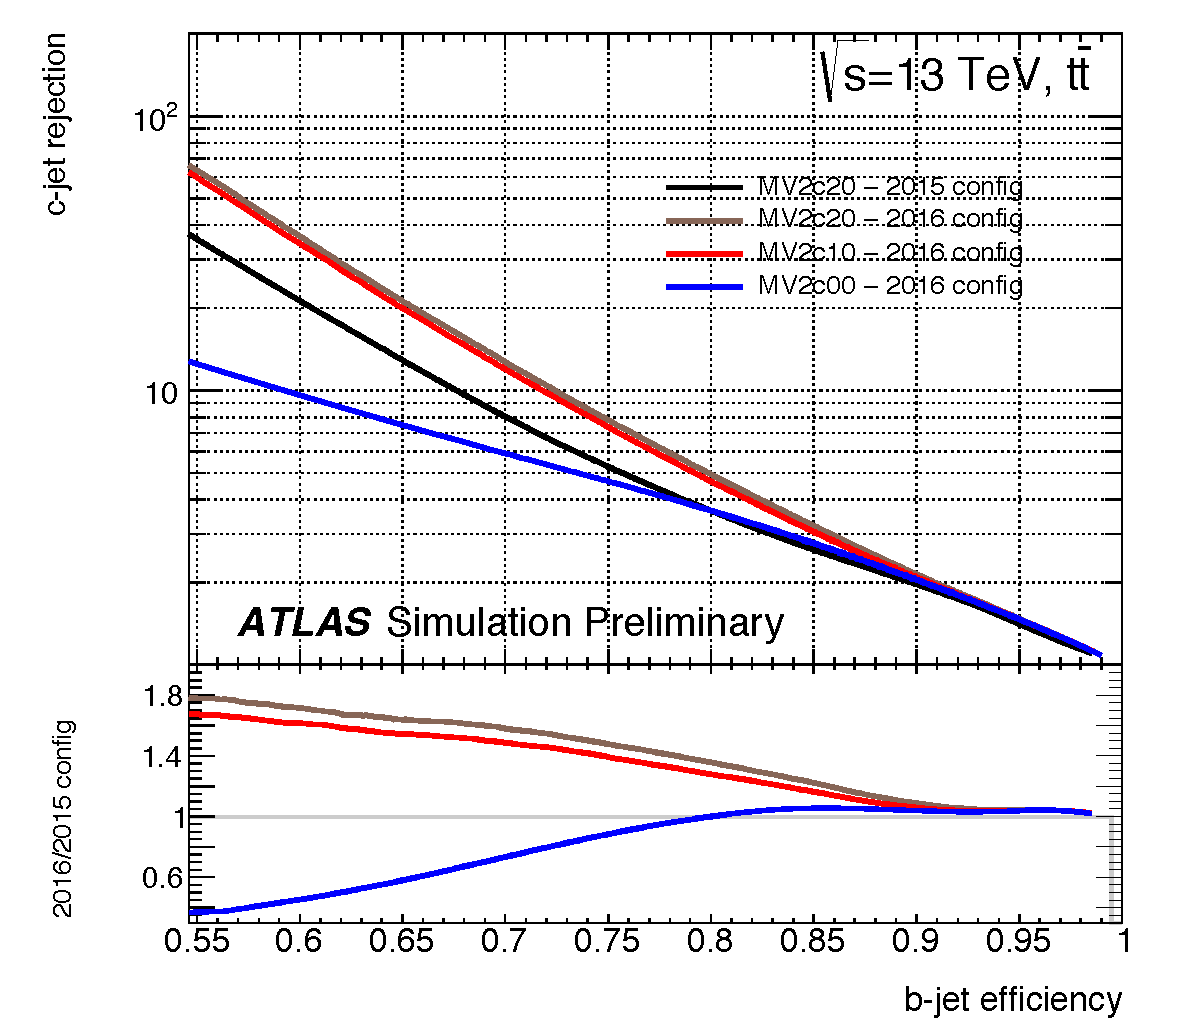
\includegraphics[width=0.48\textwidth]{figures/objects/mv2c10_b.pdf} }
\end{center}
 \caption{Light-jet \subref{fig:obj:mv2_a} and $c$-jet \subref{fig:obj:mv2_b} rejection as a function of the $b$-jet efficiency for the MV2 algorithms. Figures from Ref. \cite{ATL-PHYS-PUB-2016-012}.}
  \label{fig:obj:mv2}
\end{figure}

\glspl{op} are defined by a selection on the value of the \gls{bdt} output, and are designed to have a specific $b$-jet efficiency.
Table \ref{tab:obj:mv2op} shows the \glspl{op} of the MV2c10 algorithm.

\begin{table}[h]
\begin{center}
    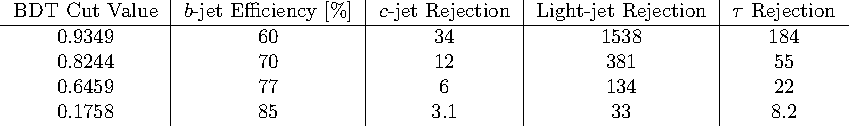
\includegraphics[width=1.0\textwidth]{figures/objects/btag_op.pdf}  
\end{center}
 \caption{Operating points for the MV2c10 $b$-tagging algorithm. The efficiency and rejection rates are computed for jets with $\pt > 20$ GeV from \ttbar events. Table from Ref. \cite{ATL-PHYS-PUB-2016-012}.}
  \label{tab:obj:mv2op}
\end{table}

\subsection{B-tagging calibration and uncertainties}
\label{sec:obj:btaggingcalib}

The $b$-tagging efficiency can be different in \gls{mc} simulation and data. The $b$-tagging efficiency, 
$c$-tagging efficiency and light mistag rate are measured in data for the \glspl{op} of Table \ref{tab:obj:mv2op}, 
and the \gls{mc} simulation is corrected with the \glspl{sf} derived as the ratio of the efficiency in data and in \gls{mc}. 
The \glspl{sf} are derived on a per-jet basis in a parametric form based on jet \pt, $\eta$ and truth flavor. 
For each \gls{mc} simulated event, an event-level \gls{sf} is derived by multiplying all the efficiency \glspl{sf} for the $b$-tagged jets 
and all the inefficiency \glspl{sf} for the jets that are not $b$-tagged. Different techniques are used in \gls{atlas} to measure the $b$-tagging 
efficiency in \gls{atlas} for the different jet flavors \cite{1748-0221-11-04-P04008}.
The calibrations used in the analyses described in this thesis are:

\begin{description}

\item[$b$-jets] The default $b$-tagging calibration for $b$-jets is based on a \ttbar dileptonic sample. Events with exactly two opposite-sign leptons
and two or three jets are selected, and a per-event likelihood is built containing the $b$-tagging weight \gls{pdf} for a jet of a given flavor;
the \gls{pdf} for light-jets and $c$-jets is taken from \gls{mc}, while the \gls{pdf} for $b$-jets is the information that we want to extract from data.
This last \gls{pdf} is described by a histogram with only two bins, one below and one above the threshold to $b$-tag a jet. 

%\gls{bdt} based on 8 input variables 
%Likelihood fit using per-jet flavor correlations. 

\item[$c$-jets] The analysis described in Chapter \ref{chap:strong_prod} uses a $c$-jet calibration based on events where a $W$ boson 
is produced in association with a $c$-quark. The events selected are the ones where the $W$ boson decays into an electron and a neutrino,
and the D-hadron originating from the fragmentation of the $c$-quark decays to a muon. 
In $W+c$ production the electron and the muon in the final state have opposite charge, 
while most of the background processes have an equal number of same-sign and opposite-sign events. The number of $W+c$ events can therefore 
be obtained as the difference of these two categories.
For the Higgsino search described in Chapter \ref{chap:ewk_prod}, which was developed at a later time, a new calibration for $c$-jets, 
based on \ttbar events \cite{ATLAS:2018bpl}, was available. 
This calibration selects \ttbar events where one of the $W$ bosons decays leptonically and the other one decays to a $c$-quark and an s-quark. 

\item[light-jets] The $b$-tagging efficiency of light-jets (mistag rate) is measured on an inclusive sample of jets, using the negative tag method 
\cite{ATLAS:2018xcf}. 
The two main reasons that lead to $b$-tagged light-jets are the finite resolution of the impact parameter and the secondary vertices caused
by long-lived particles and material interactions. If we consider only the first type of mistags, the signed impact parameter distribution 
will be symmetric around zero. 
The negative tag method is based on a modified version of the $b$-tagging algorithms, that takes as input impact parameters and decay lengths with
reversed sign. The mistag rate is measured as the negative-tag efficiency of the jet sample, with \gls{mc}-based correction factors that take into account 
the negative-tag rate for $b$- and $c$-jets and the effect of long-lived particles and material interactions.

\end{description}

The $b$-tagging scale factors are affected by multiple sources of uncertainty, which are reflected in uncertainties on the \glspl{sf}.
As an example, Figure \ref{fig:obj:btagSF} shows the $b$-tagging \gls{sf} for $c$-jets derived with the \ttbar calibration 77\% \gls{op}, 
and Figure \ref{fig:obj:mistagSF} shows the \glspl{sf} for light-jets derived with the negative tag calibration for the same \gls{op}.

%\note{Plots for other calibrations will be added after CONF are public (should be LHCP)}.

\begin{figure}[htbp]
\begin{center}
  %\subfigure[]{
  %  \label{fig:obj:ttSF}
    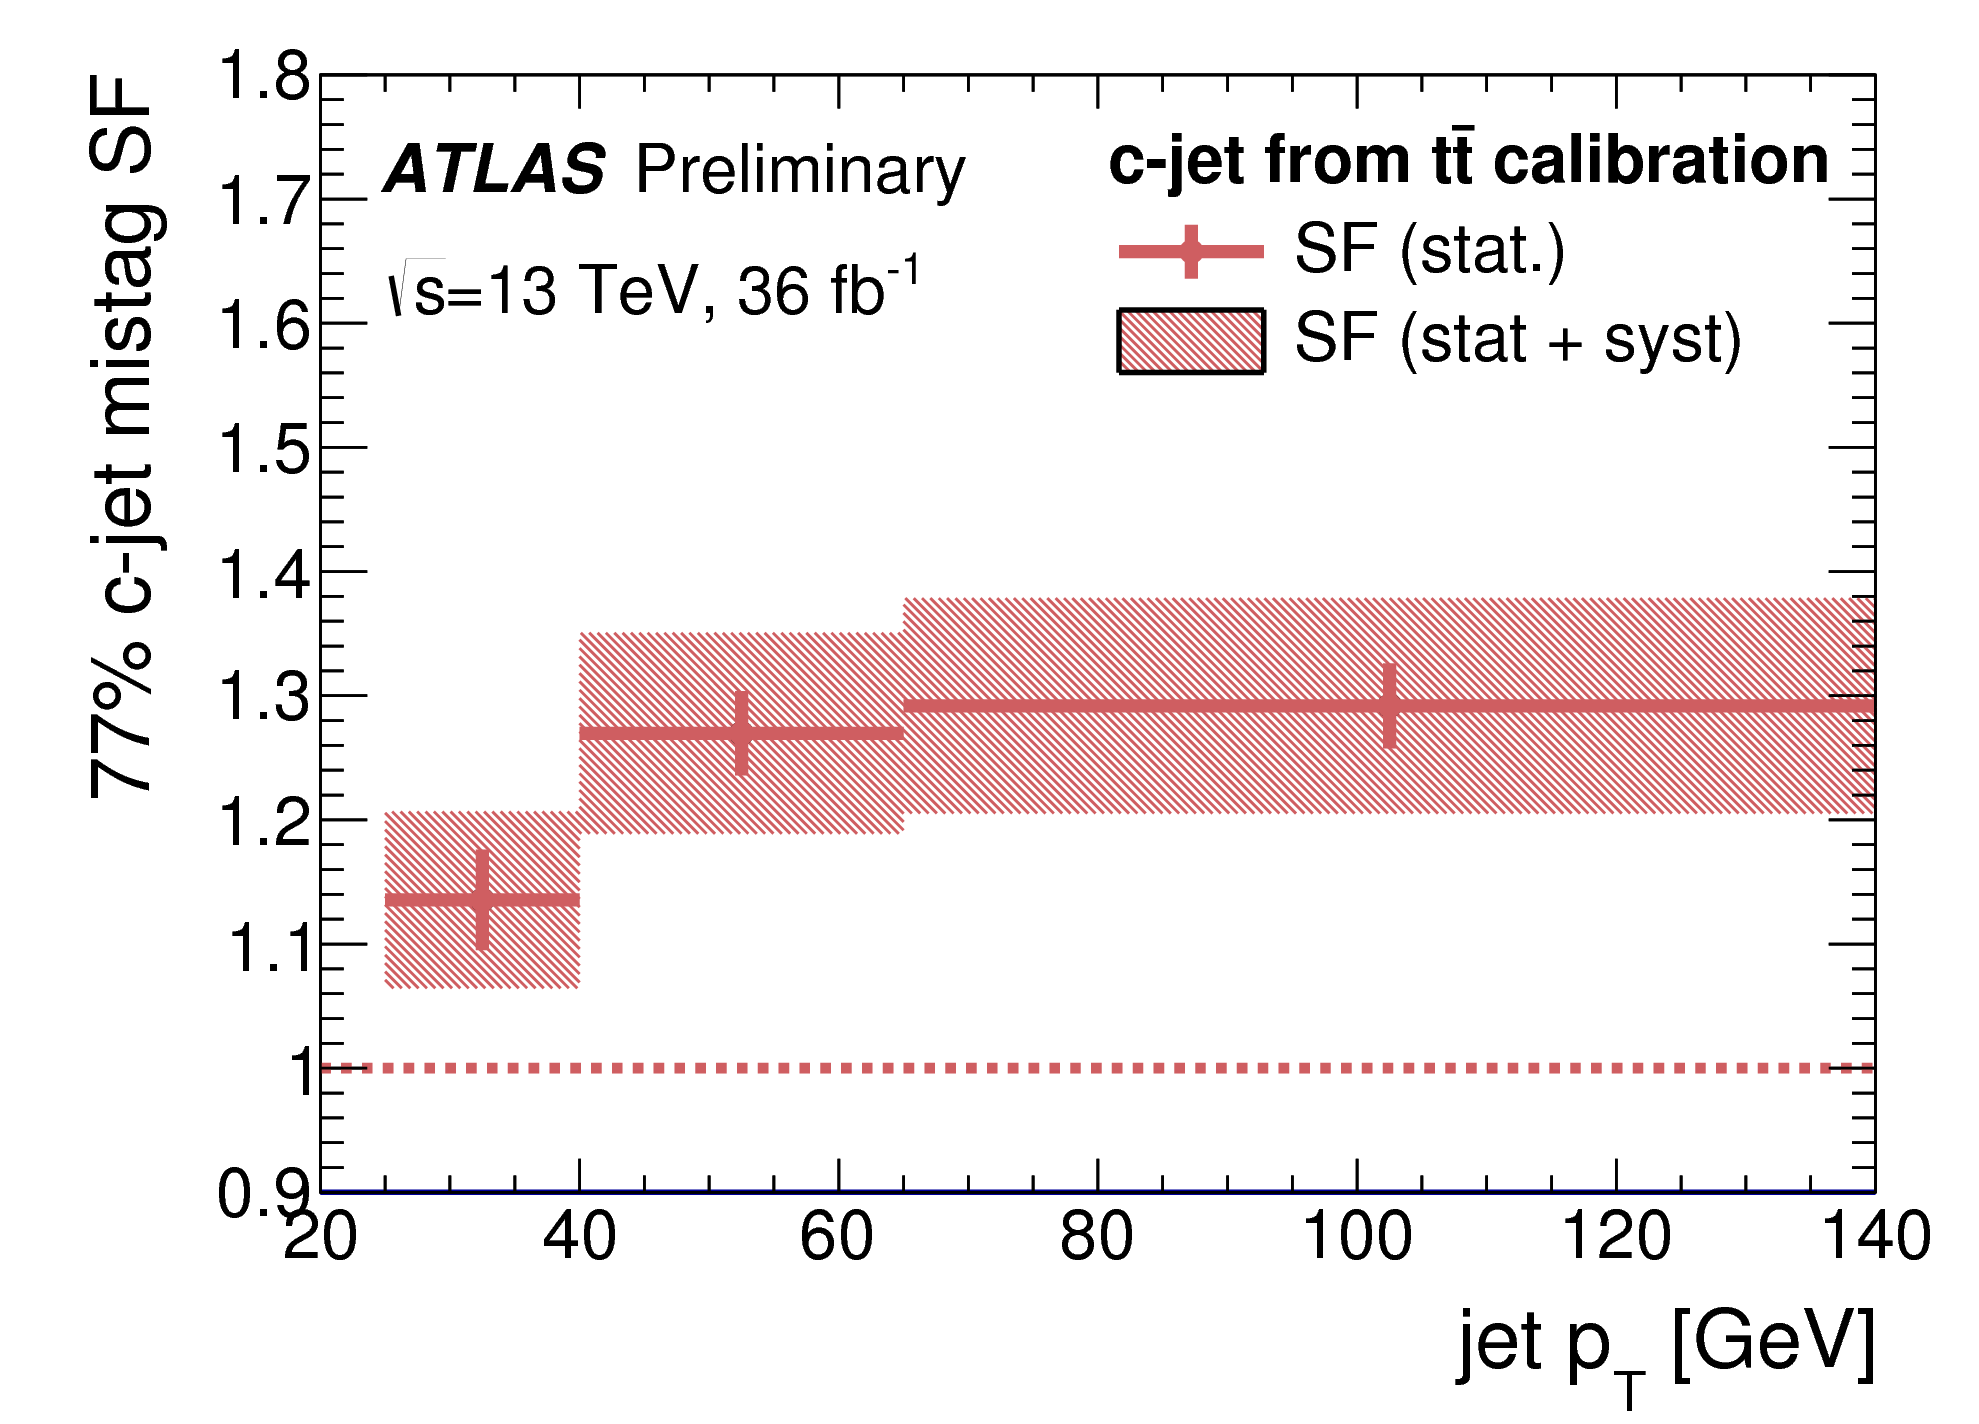
\includegraphics[width=0.48\textwidth]{figures/objects/cjettt_77SF.png}  %}
  %\subfigure[]{
   % \label{fig:obj:mv2_b}
    %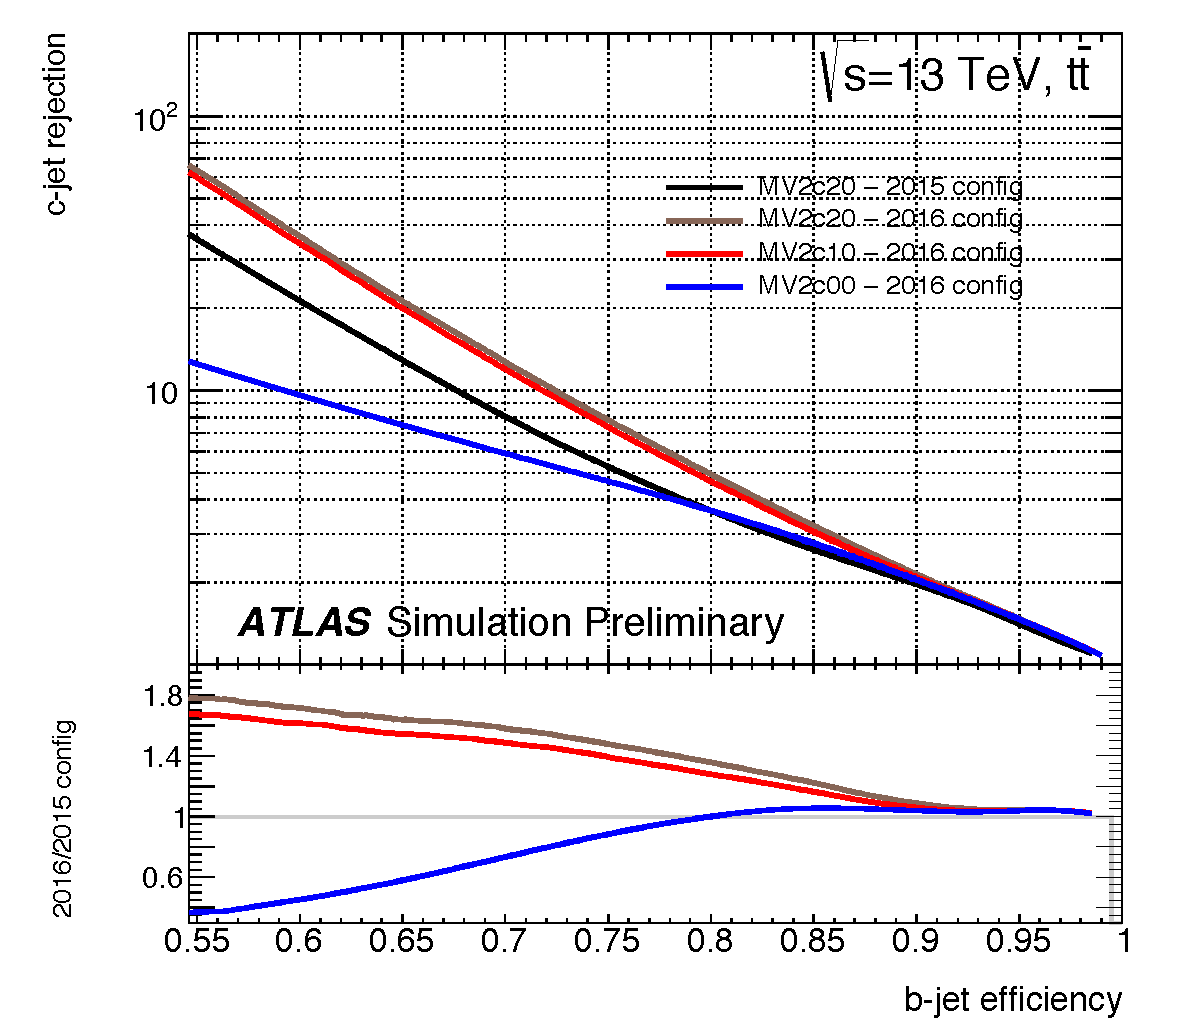
\includegraphics[width=0.48\textwidth]{figures/objects/mv2c10_b.pdf} }
\end{center}
 \caption{$B$-tagging \gls{sf} for $c$-jets for the \gls{op} corresponding to the 77\% \gls{op}. Figure from Ref. \cite{ATLAS:2018bpl}.}
  \label{fig:obj:btagSF}
\end{figure}

\begin{figure}[htbp]
\begin{center}
  \subfigure[]{
    \label{fig:obj:mistag1}
    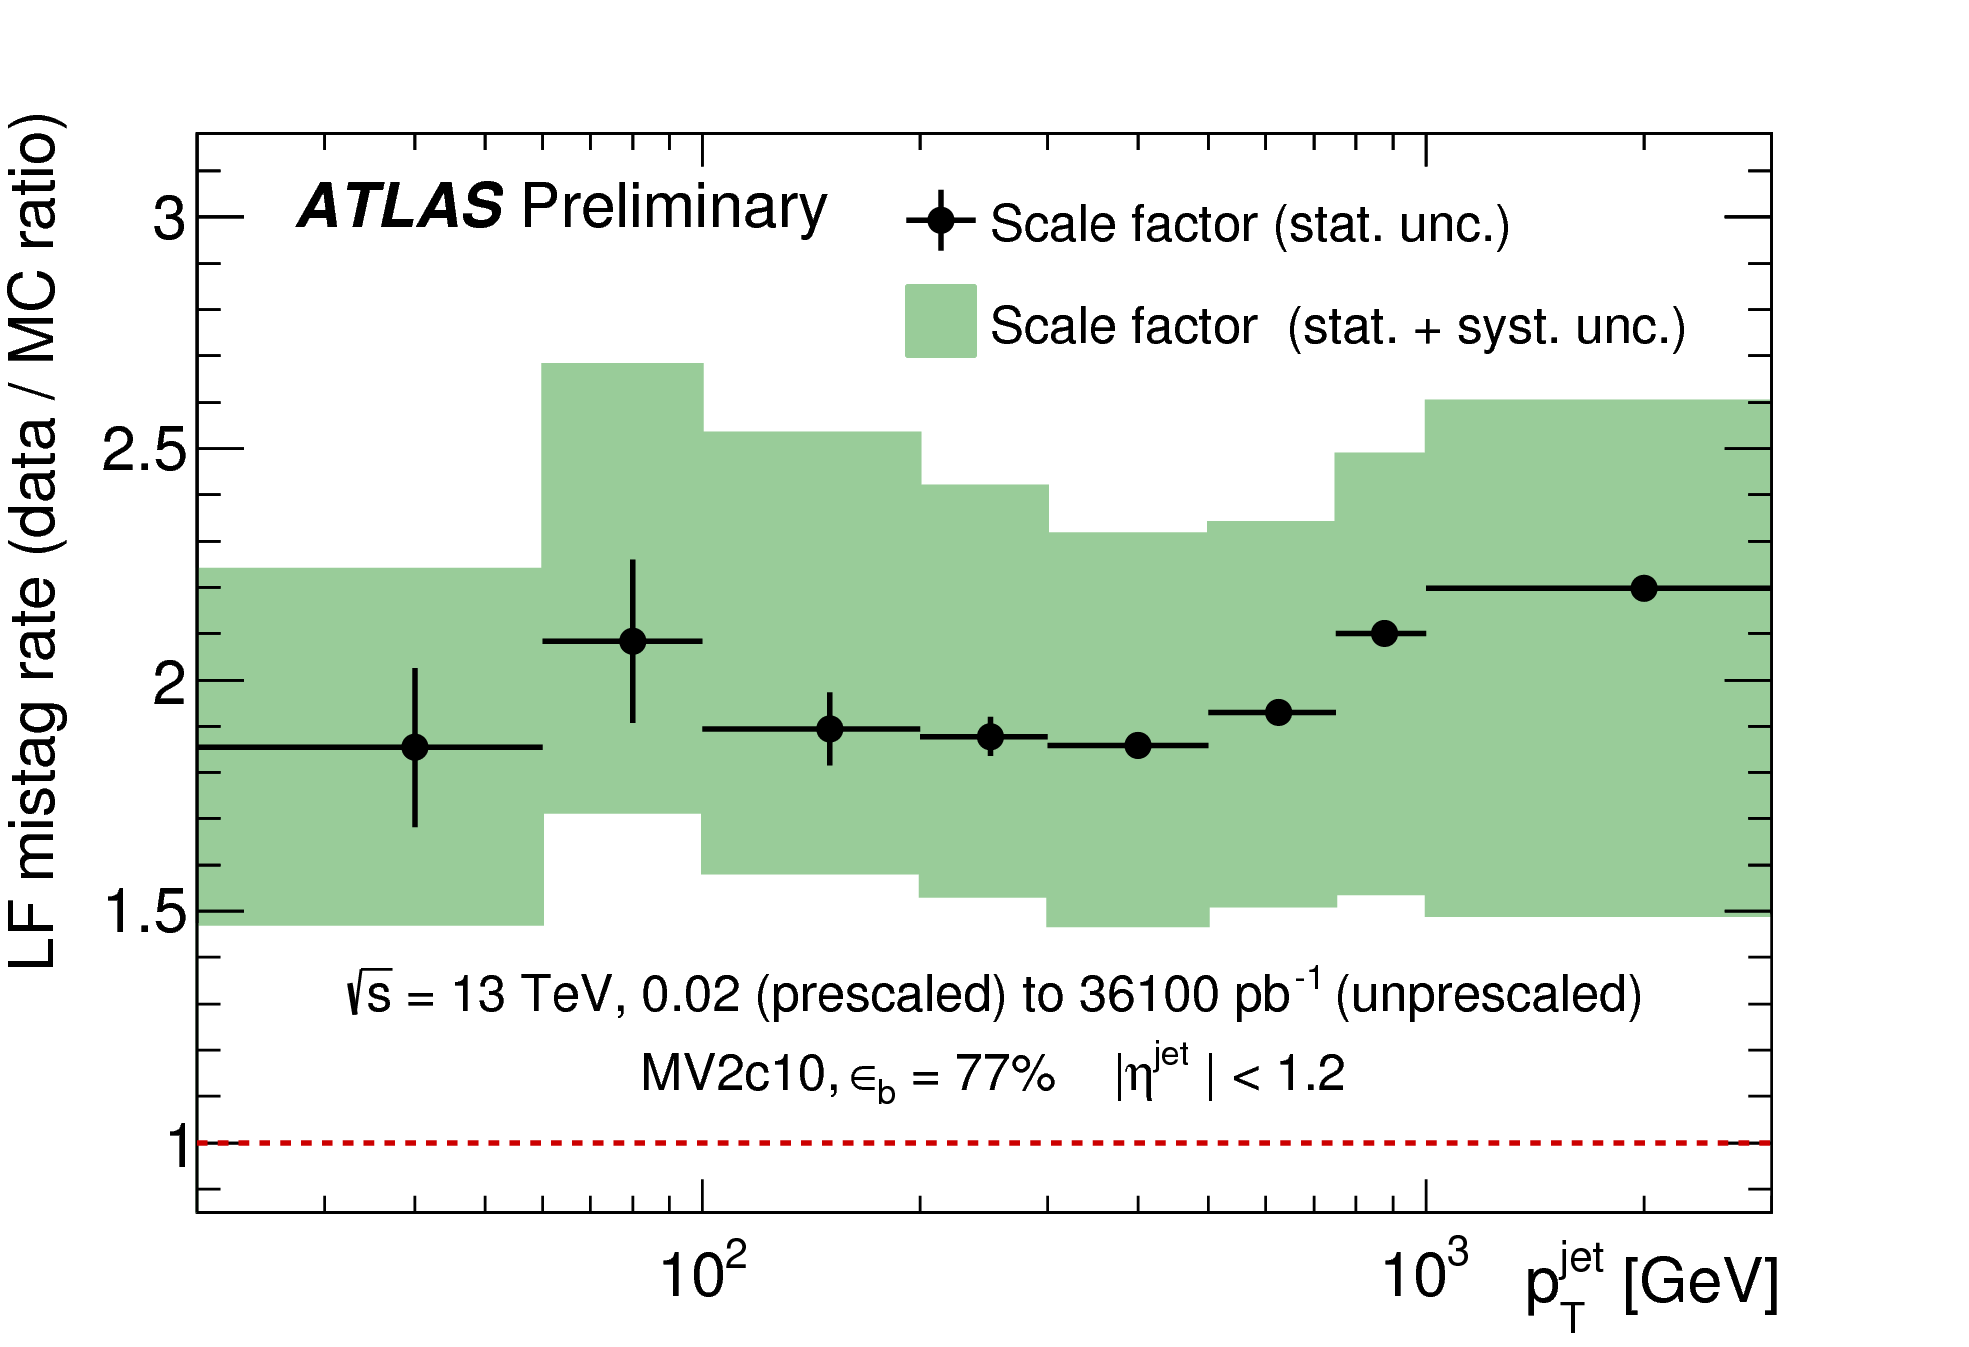
\includegraphics[width=0.48\textwidth]{figures/objects/mistag_fig_05c.png}  }
  \subfigure[]{
    \label{fig:obj:mistag2}
    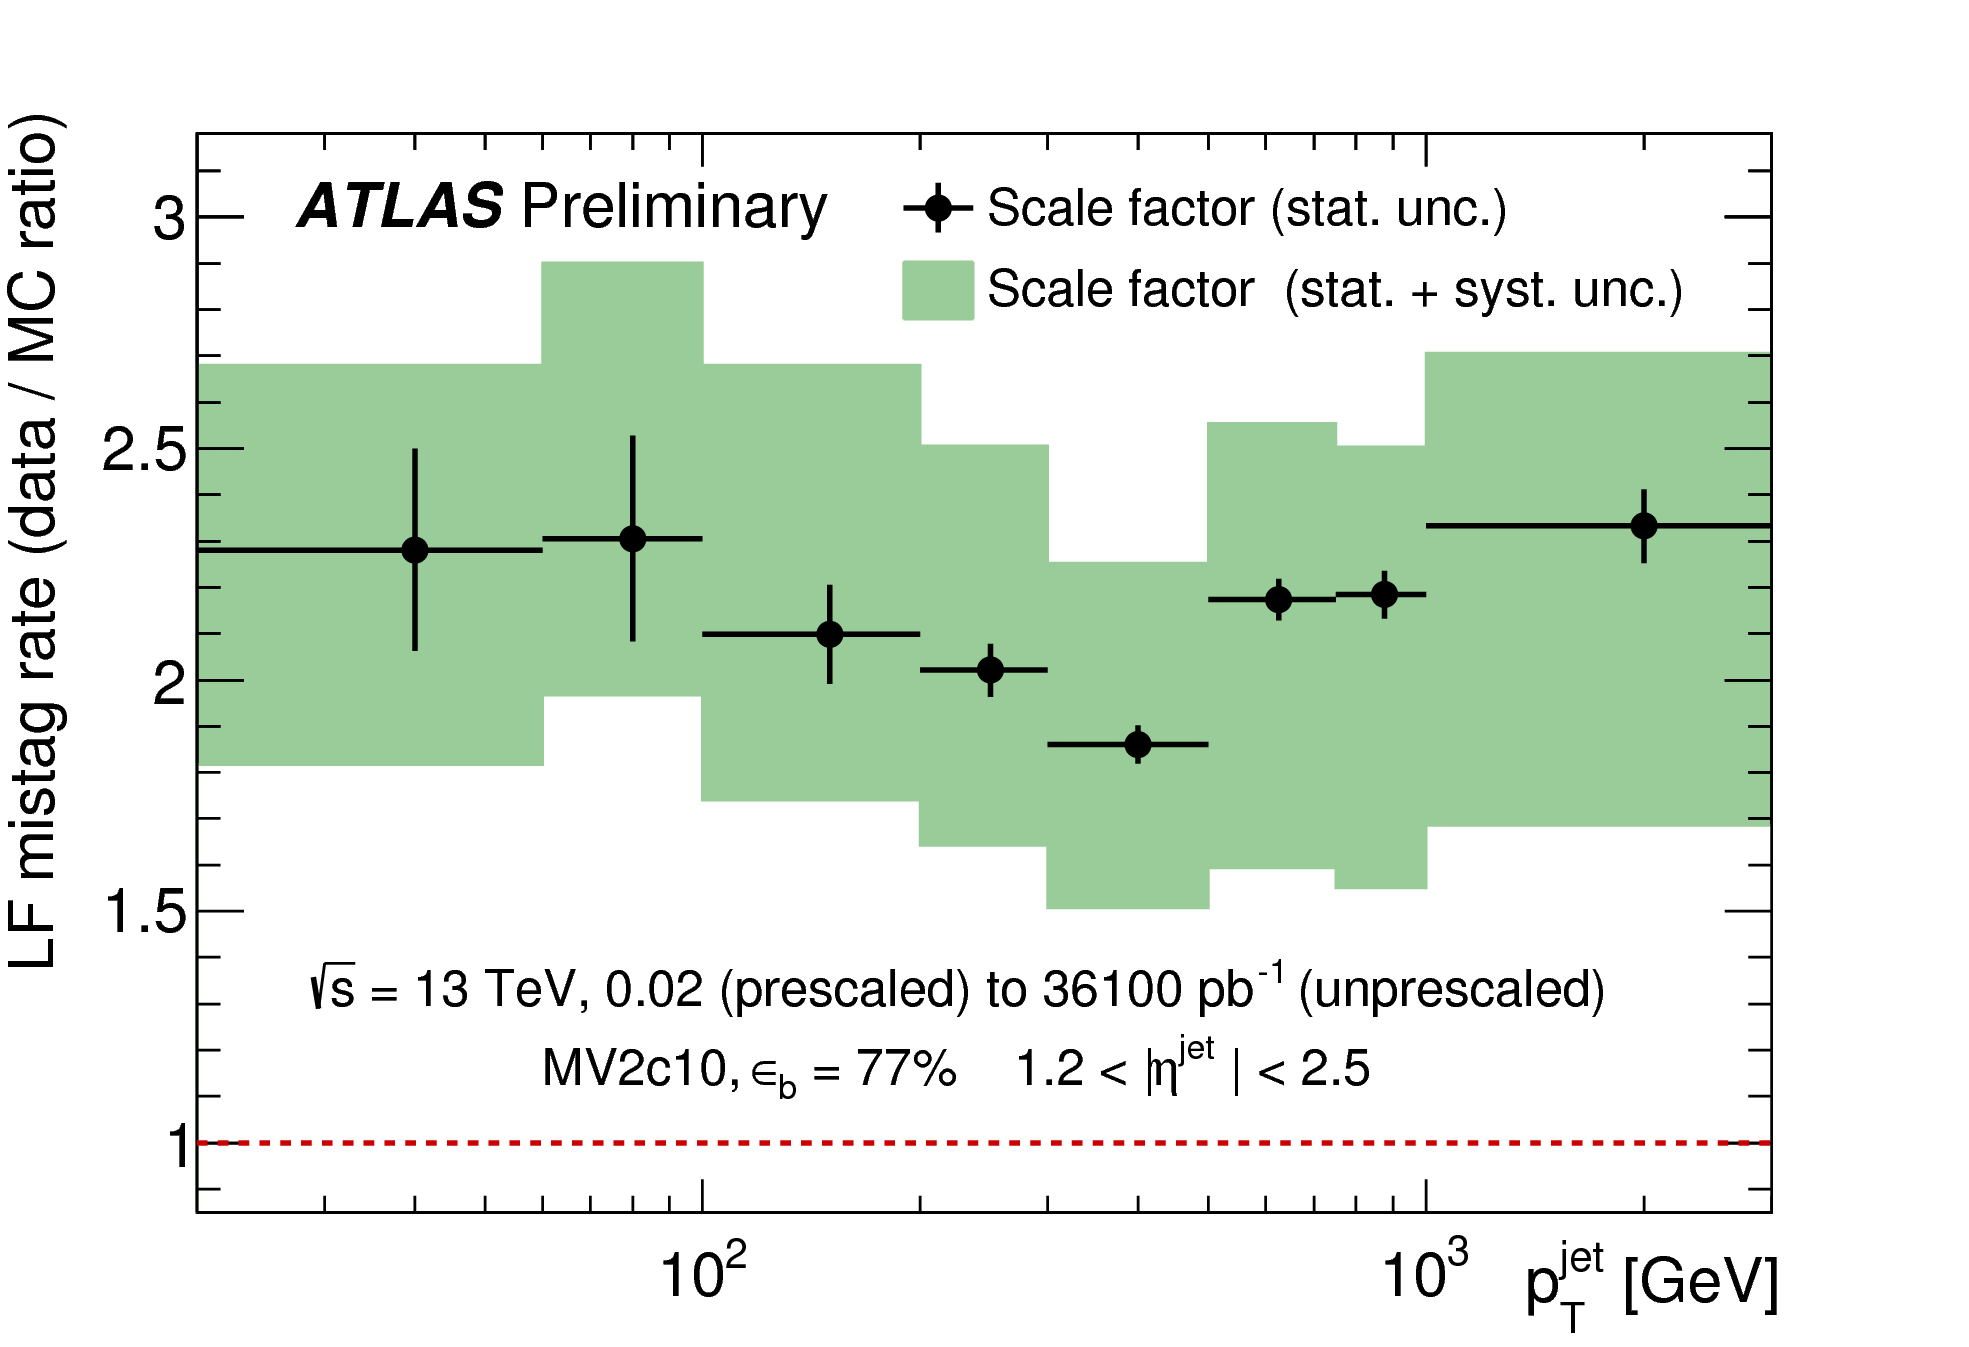
\includegraphics[width=0.48\textwidth]{figures/objects/mistag_fig_05d.png} }
\end{center}
 \caption{$B$-tagging \gls{sf} for light-jets for the \gls{op} corresponding to the 77\% \gls{op} for \subref{fig:obj:mistag1} 
 $|\eta|<1.2$ and \subref{fig:obj:mistag2} $1.2 < |\eta| < 2.5$. Figures from Ref. \cite{ATLAS:2018xcf}.}
  \label{fig:obj:mistagSF}
\end{figure}


\section{Muons}

Muon reconstruction and identification \cite{Aad:2016jkr} is based on the information collected by the \gls{id}, where muons are reconstructed as charged tracks, and by the \gls{ms}. 

\subsection{Muon reconstruction}

Both the \gls{id} and the \gls{ms} perform the reconstruction
of muon candidates independently and then the information is combined to build the muon candidates used in physics analyses. 
The reconstruction of muon tracks in the \gls{id} proceeds as described in Section \ref{sec:reco:tracks}. In the \gls{ms}, the first step is the identification of segments starting from the hits in each chamber. A muon track is reconstructed with a segment-seeded search (considering first the segments in the central layers of the detector as seeds, and then extending to the inner and outer ones). Except from the transition region between the barrel and the end-cap, tracks are required to have at least two matching segments; the hits associated to each track are fitted with a global \chis, and the track candidate is accepted or rejected based on the \chis value. 

Reconstructed muons can belong to four different types, depending on the subdetectors that contribute to their reconstruction:

\begin{description}
\item [Combined] Combined muons are built from a global fit that uses hits from tracks reconstructed independently in the \gls{id} and \gls{ms}.
\item[Segment-tagged] Muons of lower \pt or that cross regions of lower acceptance of the \gls{ms} can result in a segment in only one \gls{ms} chamber. If a track from the \gls{id} is associated with this segment, this track is classified as a segment-tagged muon.
\item[Calorimeter-tagged] A track in the \gls{id} is identified as a calorimeter-tagged muon if it is matched to an energy deposit in the calorimeter compatible with a minimum-ionizing particle. This muon category recovers identification efficiency for the muons that fall out of the \gls{ms} acceptance.
\item[Extrapolated] Extrapolated muons are reconstructed from tracks in the \gls{ms} compatible with originating from the \gls{ip}, to recover muons in high-$\eta$ regions, outside of the \gls{id} acceptance.
\end{description}

When multiple types of muon are reconstructed for the same physical object, the redundant ones are removed with an \gls{or} procedure that, when muons share the same \gls{id} tracks, gives priority to combined muons, and then to segment-tagged muons over combined muons. The \gls{or} with extrapolated muons gives preference to the \gls{ms} track with the best quality.

\subsection{Muon identification}
\label{sec:muon_id}

The reconstructed muons have to fulfill identification criteria that help reject the background constituted mostly by decays of pions and kaons. 
The variables used in the identification are the significance of the difference of the charge-over-momentum ratios measured by the \gls{id} and by the \gls{ms} ($q/p$ significance),
the difference of the \pt measured in the \gls{id} ad in the \gls{ms} divided by the \pt of the combined track ($\rho'$),
the normalized \chis of the combined fit,
and the number of hits in the different detector layers. 
Based on these quantities, four muon identification criteria are defined: Loose, Medium, Tight and High-\pt. 
Loose, Medium and Tight are inclusive categories with increasingly tighter requirements, while the High-\pt selection starts from the Medium selection and applies extra requirements that improve the momentum resolution for muons with \pt above 100 GeV.

The Medium identification criteria is the default in \gls{atlas}, and is the one that minimizes the systematic uncertainties associated with 
the muon reconstruction and calibration. In the pseudorapidity region with $|\eta|<2.5$, Medium muons are required to be combined muons with $\geq$ 3 hits in at least two \gls{mdt} layers (except for muons with $|\eta|<0.1$, in which case the requirement becomes on one \gls{mdt} layer, but with a hole veto), while extrapolated muons are used when $2.5<|\eta|<2.7$. To suppress muons from hadron decays, the $q/p$ significance is required to be less than seven. 

\subsection{Muon efficiency measurement}

In the region with $|\eta|<2.5$, where the information from both the \gls{id} and the \gls{ms} is available, 
the reconstruction efficiency is measured with a tag-and-probe method, performed on $J/\Psi \rightarrow \mu \mu$ and $Z\rightarrow \mu \mu$ events for low-\pt and high-\pt muons respectively. 
After a selection on the event topology to reduce the background fraction, one of the two muons of the decay is required to be identified 
as a Medium muon (denoted as tag muon). 
The second leg of the decay (denoted as probe muon) has to be reconstructed by a system independent on the one to be calibrated. For example, calorimeter muons can be used to measure the efficiency of muon identification in the \gls{ms}, while the \gls{id} efficiency can be measured with respect to muons identified in the \gls{ms}. 
The reconstruction efficiency of the Medium \gls{op} as derived from $Z\rightarrow \mu \mu$ and $J/\Psi \rightarrow \mu \mu$ events is shown in Fig \ref{fig:obj:muon_reco}.
The efficiency for high-$\eta$ muons, for which the \gls{id} information is not available, is measured following the strategy detailed in Ref. \cite{Aad:2014rra}.

\begin{figure}[h]
\begin{center}
  \subfigure[]{
    \label{fig:obj:muon_reco}
    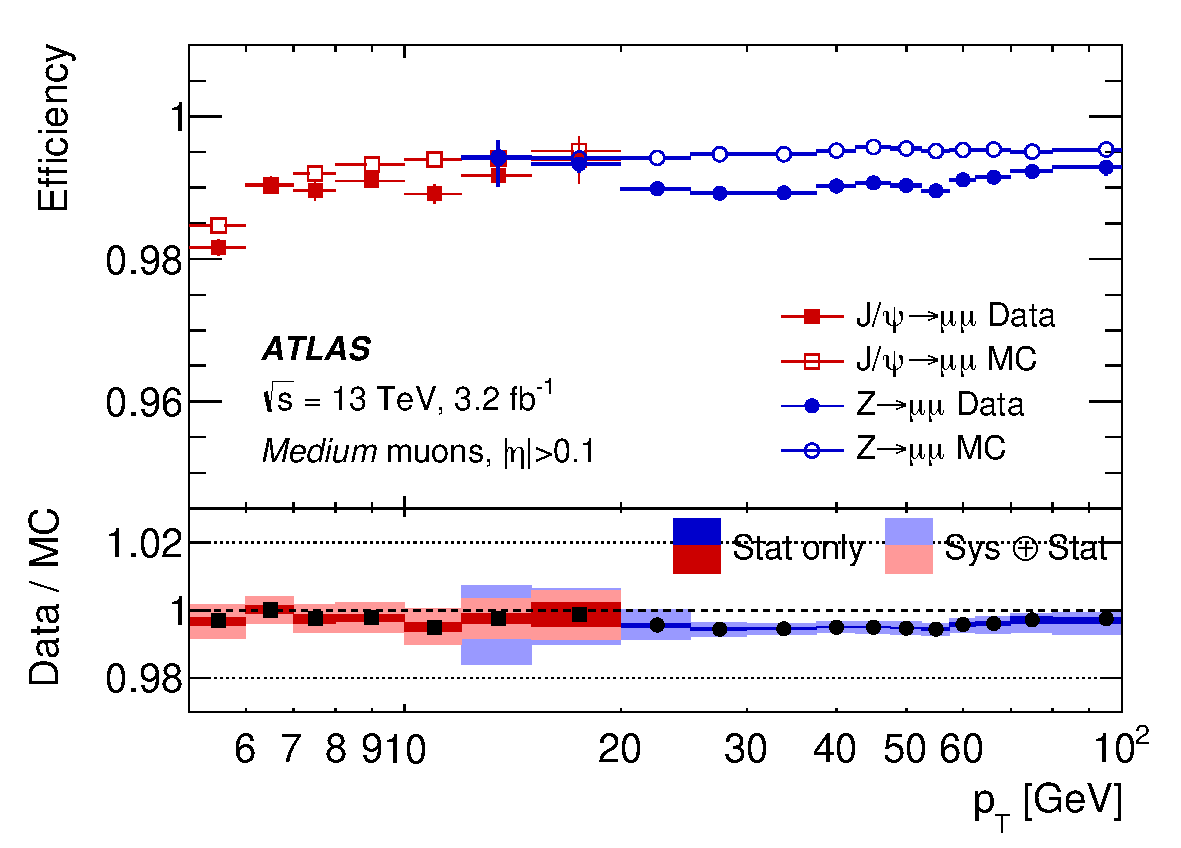
\includegraphics[width=0.48\textwidth]{figures/objects/muon_reco.eps} }
  \subfigure[]{
    \label{fig:obj:muon_iso}
    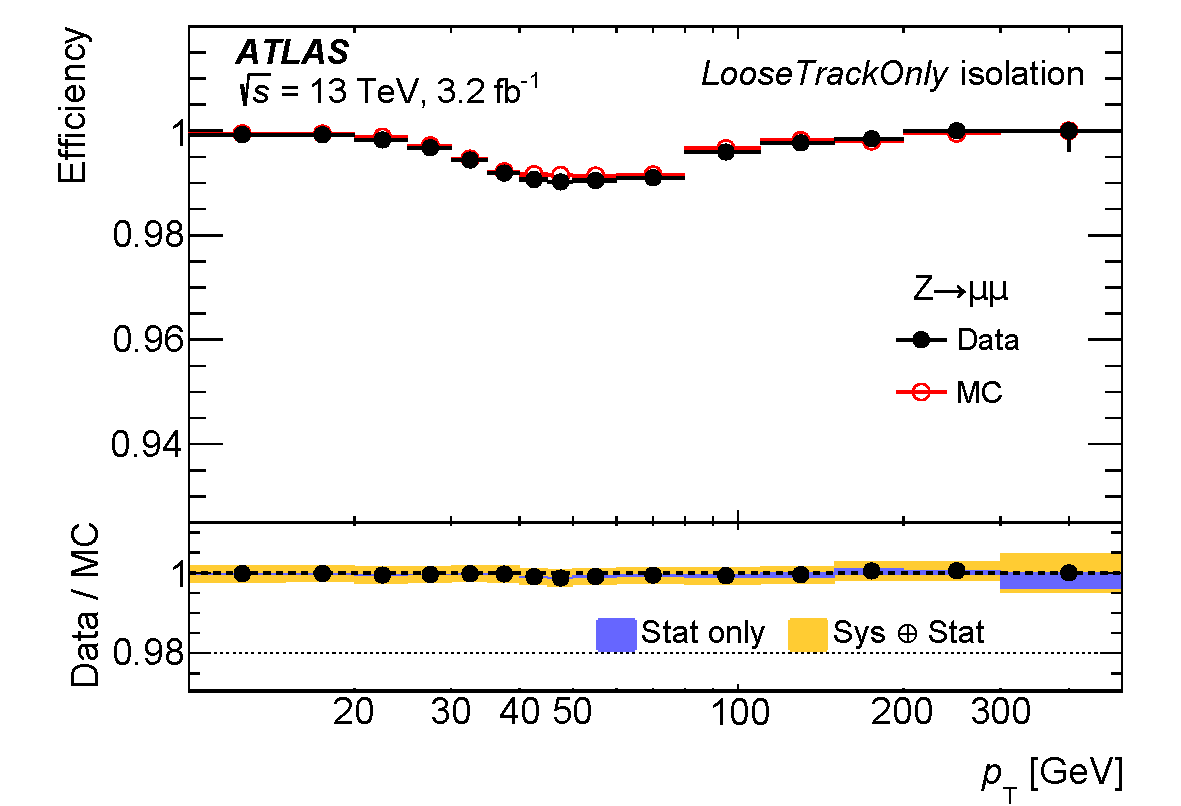
\includegraphics[width=0.48\textwidth]{figures/objects/muon_iso.eps}  }
\end{center}
 \caption{ \subref{fig:obj:muon_reco} Reconstruction efficiency for the Medium muon selection as a function of the muon \pt, in the region with $0.1<|\eta|<2.5$, as derived from $Z\rightarrow \mu \mu$ and $J/\Psi \rightarrow \mu \mu$ events. 
 \subref{fig:obj:muon_iso} Efficiency of the muon isolation criteria for the $LooseTrackOnly$ \gls{op} as derived from $Z\rightarrow \mu \mu$  events.
 In both figures, the top panel shows the efficiency for data and \gls{mc}, while the bottom panes shows the ratio of data to \gls{mc} with the corresponding uncertainty.
 Figures from Ref. \cite{Aad:2016jkr}.}
  \label{fig:obj:muon}
\end{figure}

\subsection{Muon isolation}
\label{sec:muoniso}

While muons originating from semileptonic decays of hadrons are very close to the axis of a jet, prompt muons are typically well separated from other physics objects in the event (isolated). The isolation requirements help therefore suppressing further the background from semileptonically decaying hadrons. Different isolation requirements are available and calibrated in \gls{atlas}, defined to be optimal for different analyses. 
The \gls{op} used in the analyses described in this thesis is the one labeled $LooseTrackOnly$, which applies a selection on the ratio of the 
variable \ptvar over the muon \pt (\ptmu), where \ptvar is defined as the scalar sum of the momenta of the tracks with $\pt>1$ GeV in the cone with 
$\Delta\mathrm{R} < \min \left(  10 \, \mathrm{GeV}/\ptmu , \, 0.3\right) $. The \pt-dependent size of the isolation cone helps in recovering efficiency for muons deriving from the decay of boosted particles. The efficiency of the isolation \glspl{op} is calibrated on $Z\rightarrow \mu \mu$ with the tag-and-probe method. The $LooseTrackOnly$ \gls{op} has an efficiency of 99\%, almost constant in $\eta$ and \pt, as shown in Figure \ref{fig:obj:muon_iso}. 

\subsection{Muon momentum calibration}
A set of corrections applied to the \gls{mc} simulation, such that after the correction the simulation describes the muon momentum and momentum resolution in data with a precision of the order of few per-mill and few percent respectively. 
The corrections are derived in $J/\Psi \rightarrow \mu \mu$ and $Z\rightarrow \mu \mu$ events, by performing a binned maximum-likelihood fit of the di-muon 
invariant mass distribution. 

\section{Electrons}

When electrons traverse the \gls{atlas} detector, they leave a track in the \gls{id} and then the energy of their \gls{em} shower is absorbed in the \gls{ecal}.

\subsection{Electron reconstruction}

The electron reconstruction \cite{ATLAS:2011lah,Aad:2014nim,ATLAS:2016iqc} starts with the identification of clusters in the \gls{ecal}. 
The \gls{ecal} can be divided in a grid of towers of size $0.025\times0.025$ in $\eta$ and $\phi$, and the tower energy is the sum of the 
energy of all the cells belonging to the tower. 
While, in the case of hadronic jets, the calorimeter clusters are created with a topological 
algorithm, in the case of electrons the calorimeter clusters are based on a sliding-window algorithm \cite{Lampl:2008zz} 
with a size of $3\times5$ in units of $0.025\times0.025$ in the ($\eta$, $\phi$) space, that searches for seed towers; these are the centers around which clusters are built.   

The identified clusters are the starting point to reconstruct electrons, photons and converted photons. The key feature that allows to separate electrons from converted and unconverted photons is that, in the case of electrons, the calorimeter clusters are associated with a track from the \gls{id}; instead, in the case of converted photons the cluster is associated with a conversion vertex, while there is no track associated to an unconverted photon. Tracks from the \gls{id} are extrapolated to the second layer of the \gls{ecal}, and a track is considered loosely matched to a seed cluster if the $\eta$ difference between the track and the barycentre of the cluster is lower than 0.05 and the $\phi$ difference either lower than 0.2 (0.1 in the case of tracks deriving from hits only in the \gls{trt}) in the bending direction, or lower that 0.05 in the opposite direction. 
The tracks loosely matched with these criteria are then re-fitted with a Gaussian Sum Filter algorithm \cite{ATLAS:2012dma}, that takes into account non-linear bremsstrahlung effects, and the re-fitted tracks are matched with 
the clusters with the same criteria as the loose matching, except from the $\phi$ difference in the direction of the bending, which is tightened to 0.1. If multiple tracks are associated to a cluster, only one is chosen as primary track based on the cluster-track distance.
After the cluster-track matching, the cluster is re-built using groups of $3\times7$ ($5\times5$) towers in the barrel (endcaps). 

Once the electron is reconstructed, its energy is obtained from the energy of calorimter cluster calibrated to the 
original electron energy with multivariate techniques \cite{Aad:2014nim}, as will be discussed in Section \ref{sec:obj:ele_energy}, while the $\eta$ and $\phi$ coordinates 
derive from the primary associated track.

Selections on the parameters of the primary track are applied to ensure that the electron is compatible with the \gls{pv} interaction. 
In particular, in Run 2 analyses these selections are: \dzero/$\sigma_\dzero < 5$ and  $\zzerost < 0.5$ mm.


\subsection{Electron identification}
\label{sec:elec_id}

After the electron candidates are reconstructed, a likelihood-based discriminant is used to reject the background, 
constituted mostly by hadronic jets and converted photons. 
This discriminant is built using as signal and background samples $Z\rightarrow e e$ and dijet events respectively for the
high-\et region, and $J/\Psi \rightarrow e e$ and minimum bias events respectively for the low-\et region.
Several variables are used to discriminate between signal and background, based on ratios of energy released in different layers of 
the calorimeter, shape of the \gls{em} shower, quality of the track and of the track-cluster matching; 
the full list of variables is reported in Table \ref{tab:obj:elev_var}.
The variables counting the number of hits in the different layers, as well as $E/p$, $w_\mathrm{stot}$ and 
$\Delta\phi_2$ are used to apply simple selections, while for the other discriminating variables \glspl{pdf} are built based
on the signal and background samples.

\begin{table}[h]
\begin{center}
    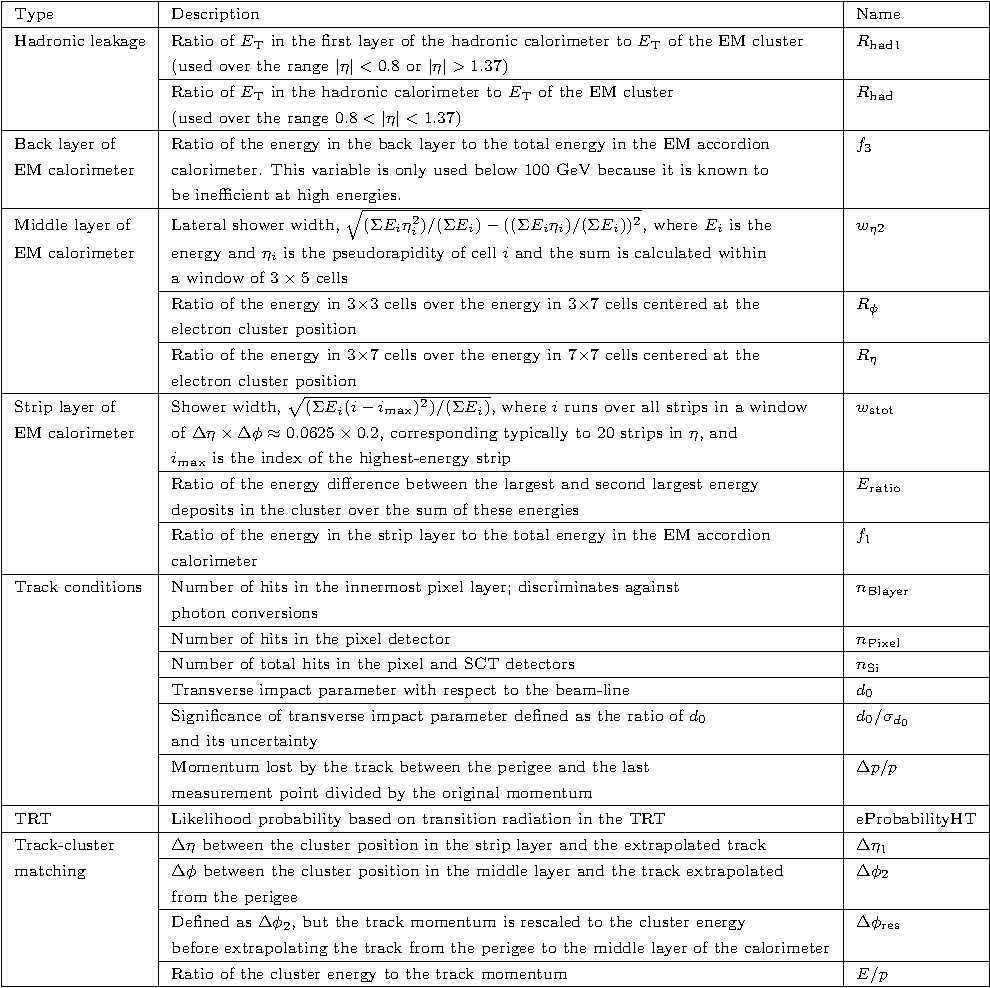
\includegraphics[width=0.985\textwidth]{figures/objects/ele_var_tab.pdf}  
\end{center}
 \caption{Definitions of electron discriminating variables. Table from Ref. \cite{ATLAS:2016iqc}.}
  \label{tab:obj:elev_var}
\end{table}

The product of these \glspl{pdf} constitutes the 
signal and background likelihoods ($\mathcal{L}\rm s$ and $\mathcal{L}\rm s$ respectively), and the final discriminant is given by:

\begin{equation}
 d_\mathcal{L} = \frac{\mathcal{L}\rm s}{\mathcal{L}\rm s + \mathcal{L}\rm b} \; .
\end{equation} 

Three identification \glspl{op} are defined, Loose, Medium and Tight, optimized in bins of $|\eta|$ and \et;
these \glspl{op} are inclusive and with an increasing level of signal purity.
The signal and background efficiency in \gls{mc} samples is shown in Figure \ref{fig:obj:ele_eff}. It is possible to notice how, with increasing
\et, the signal efficiency increases and the background mis-identification decreases.
 
\begin{figure}[h]
\begin{center}
  \subfigure[]{
    \label{fig:obj:ele_eff_e}
    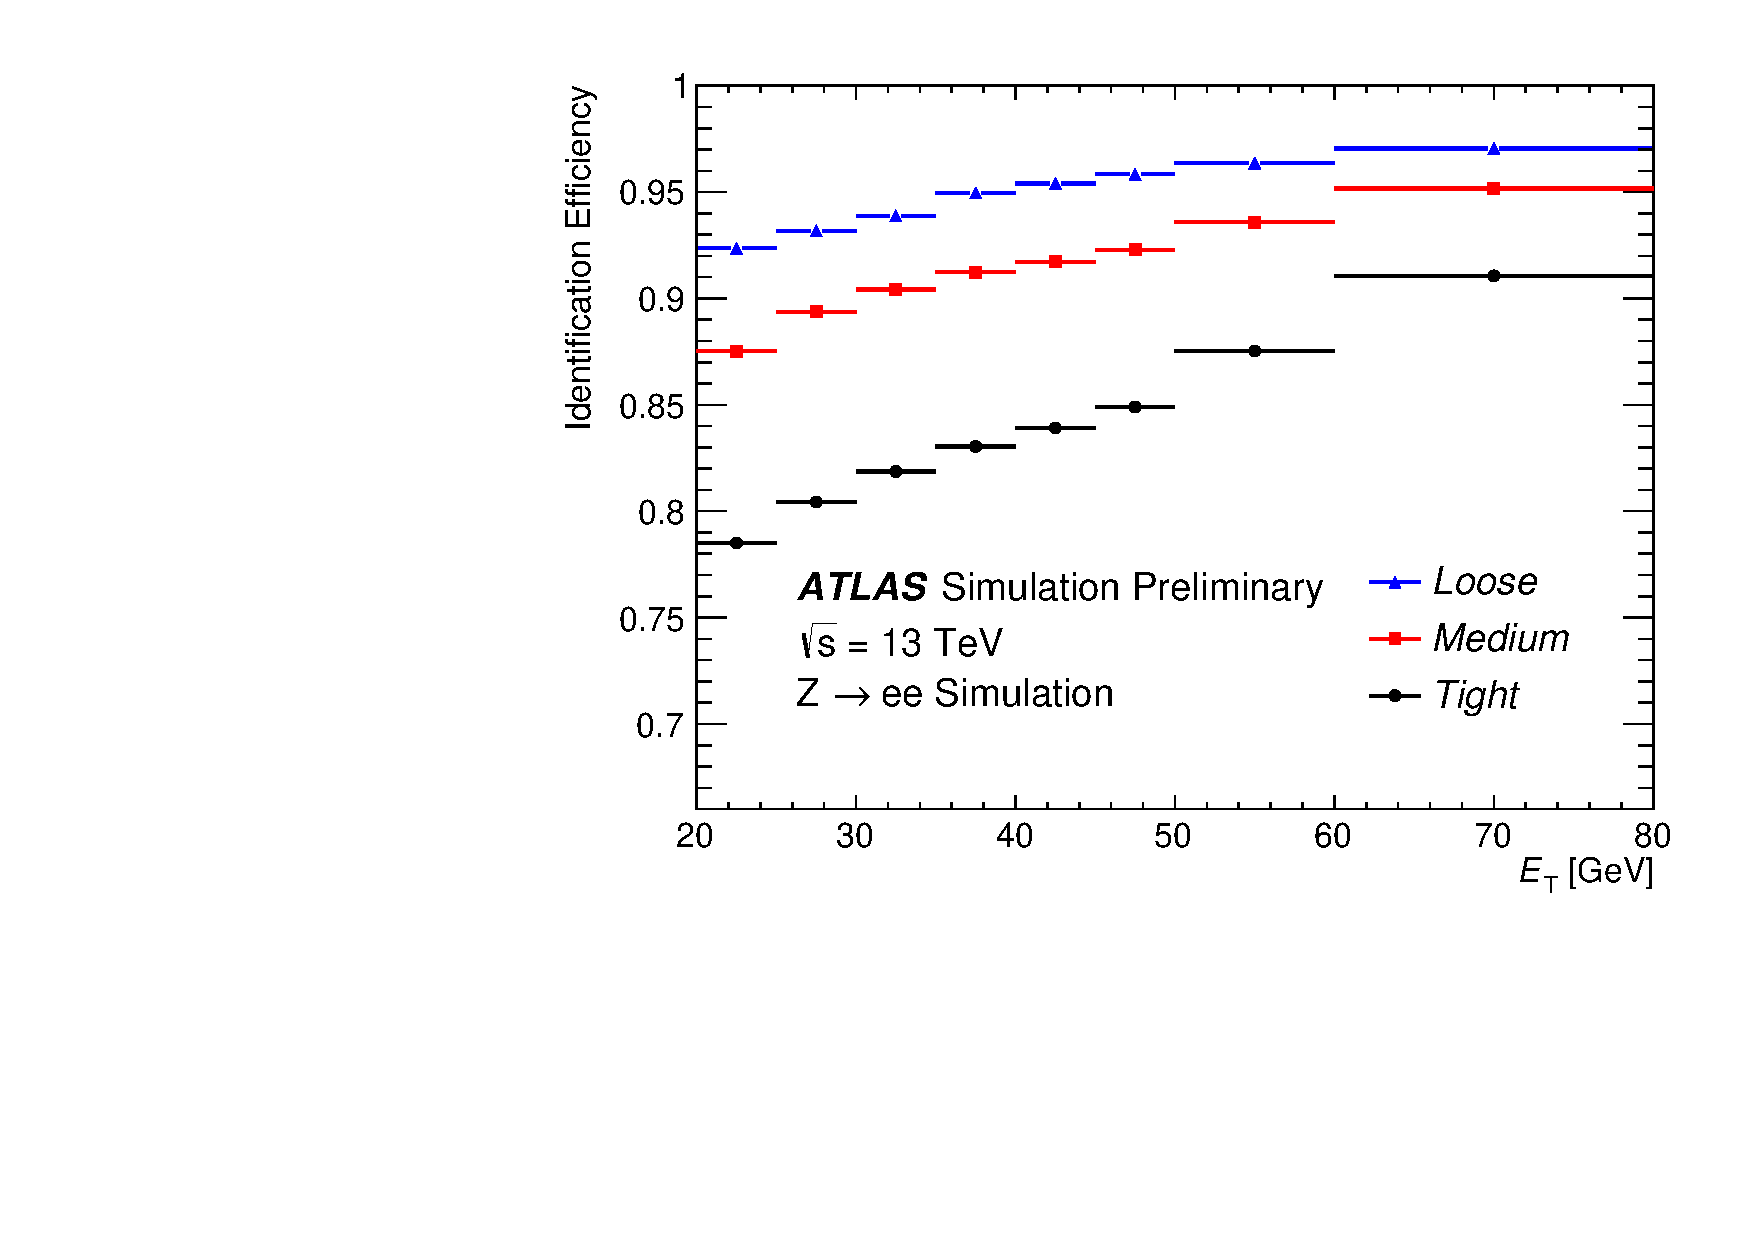
\includegraphics[width=0.48\textwidth]{figures/objects/ele_eff} }
  \subfigure[]{
    \label{fig:obj:ele_eff_bkg}
    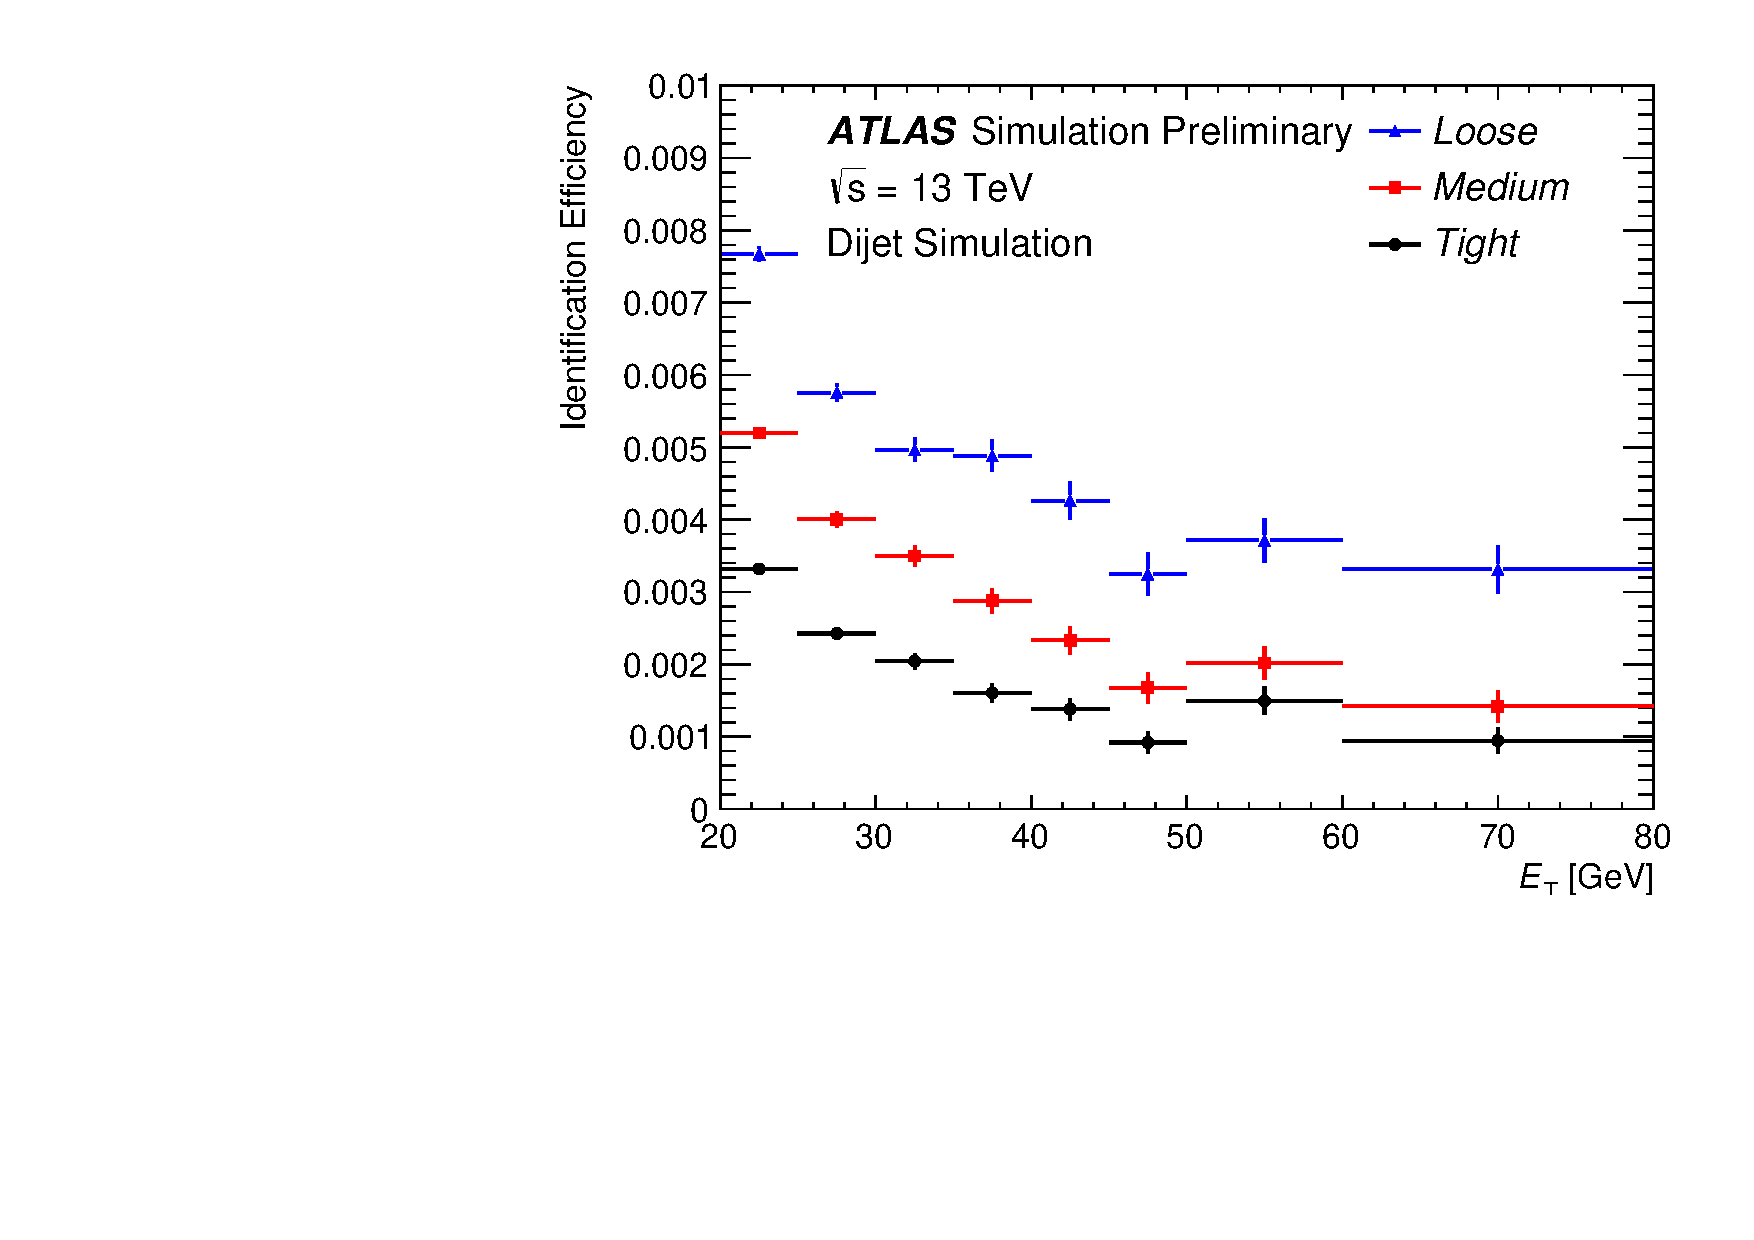
\includegraphics[width=0.48\textwidth]{figures/objects/ele_bkg_eff}  }
\end{center}
 \caption{\subref{fig:obj:ele_eff_e} Electron identification efficiency in $Z\rightarrow e e$ events and \subref{fig:obj:ele_eff_bkg} background mis-identification in dijet events for the three \glspl{op} Loose, Medium and Tight. Figures from Ref. \cite{ATLAS:2016iqc}.
 }
  \label{fig:obj:ele_eff}
\end{figure}


\subsection{Electron isolation}

As already discussed in the case of muons in Section \ref{sec:muoniso}, prompt signal electrons are in general more isolated than 
electrons candidates originating from hadron decays, from light hadrons misidentified as electrons or from photon conversion. 
The analyses described in this thesis use a track-based isolation criterion, based on the variable \ptvarele, defined as the scalar sum of the \pt 
of the tracks satisfying quality requirements in a cone with $\Delta\mathrm{R} < \min \left(  10 \, \mathrm{GeV}/\et , \, 0.2\right)$, where \et is the transverse energy of the electron candidate and the sum excludes the electron track. The operating point used is $LooseTrackOnly$, 
that applies a selection on the ratio \ptvarele/\et to have an efficiency of 99\% on simulated $Z\rightarrow e e$ events, constant as a function of \et.

\subsection{Electron efficiency measurement}

The measurement of the electron efficiency in data relies on the tag-and-probe method, applied to $Z\rightarrow e e$ and $J/\Psi \rightarrow e e$ events, for the high-\et ($> 15$ GeV) and low-\et (typically 7-20 GeV) regions respectively. One of the two electrons is identified with strict criteria and, after kinematic requirements, the second one is used to measure the efficiency.
The electron efficiency is a product of the reconstruction, identification and isolation efficiency 
(and also trigger efficiency, if the events are selected with an electron trigger).  The ratio between the efficiency expected from \gls{mc} simulations and the one measured in data, in the form of \glspl{sf} function of \et and $|\eta|$, is used to correct the simulations and its uncertainty is applied as a systematic variation. 

The identification efficiency is measured with four methods, always with respect to reconstructed electrons. Two methods, $Z_\mathrm{mass}$ and $Z_\mathrm{iso}$, use $Z\rightarrow e e$ events. 
In the $Z_\mathrm{mass}$ analysis, the tag-probe invariant mass is required to be within 15 GeV of the $Z$ boson mass, while in the $Z_\mathrm{iso}$ method the electron isolation is used to discriminate between signal and background. The other two methods \cite{ATLAS:2014wga}, $J/\Psi$ $\tau$-cut and $J/\Psi$ $\tau$-fit, use the distribution of a variable related to the $J/\Psi$ proper time (pseudo-proper time) to select $ee$ events. 
The two $Z$-based methods and the two $J/\Psi$-based methods are combined, taking into account statistical and systematic correlations, to 
derive \glspl{sf} in the high-\et and low-\et regions. 
%As an example, the identification efficiency \glspl{sf} for Tight electrons in the 40-45 \et range, measured in the 2015 data are shown in Figure \ref{fig:obj:ele_sff_tight}. 
%Figure \ref{fig:obj:ele_id2016} shows the electron identification efficiency as measured in the 2016 data, for the three \glspl{op} and inclusive in $\eta$. In this second case, the difference between data and \gls{mc} is due to the fact that \gls{mc} simulation do not reflect the changes in the \gls{trt} configuration in 2016 \cite{atlaselec2016}.

%\begin{figure}[h]
%\begin{center}
%  \subfigure[]{
%    \label{fig:obj:ele_sff_tight}
%    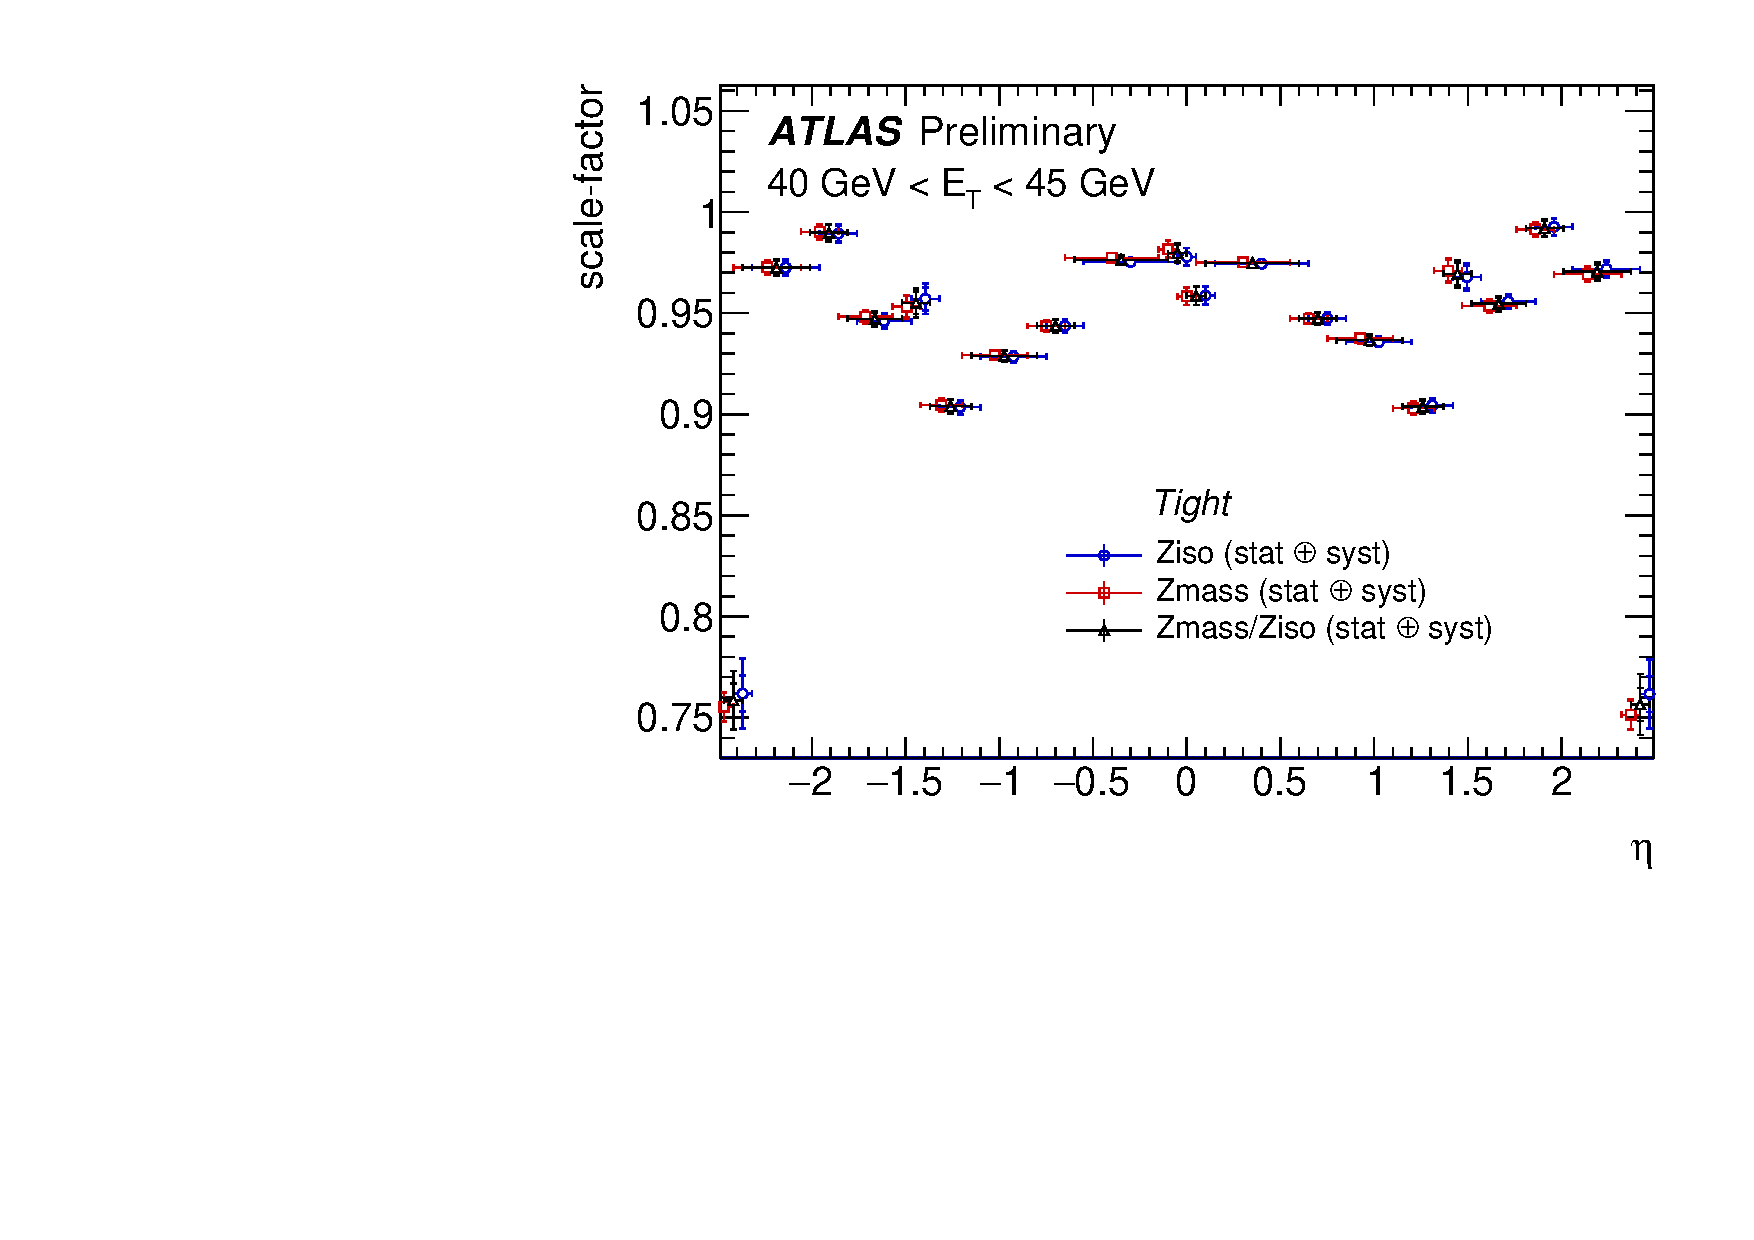
\includegraphics[width=0.51\textwidth]{figures/objects/ele_sf_tight} }
%  \subfigure[]{
%    \label{fig:obj:ele_id2016}
%    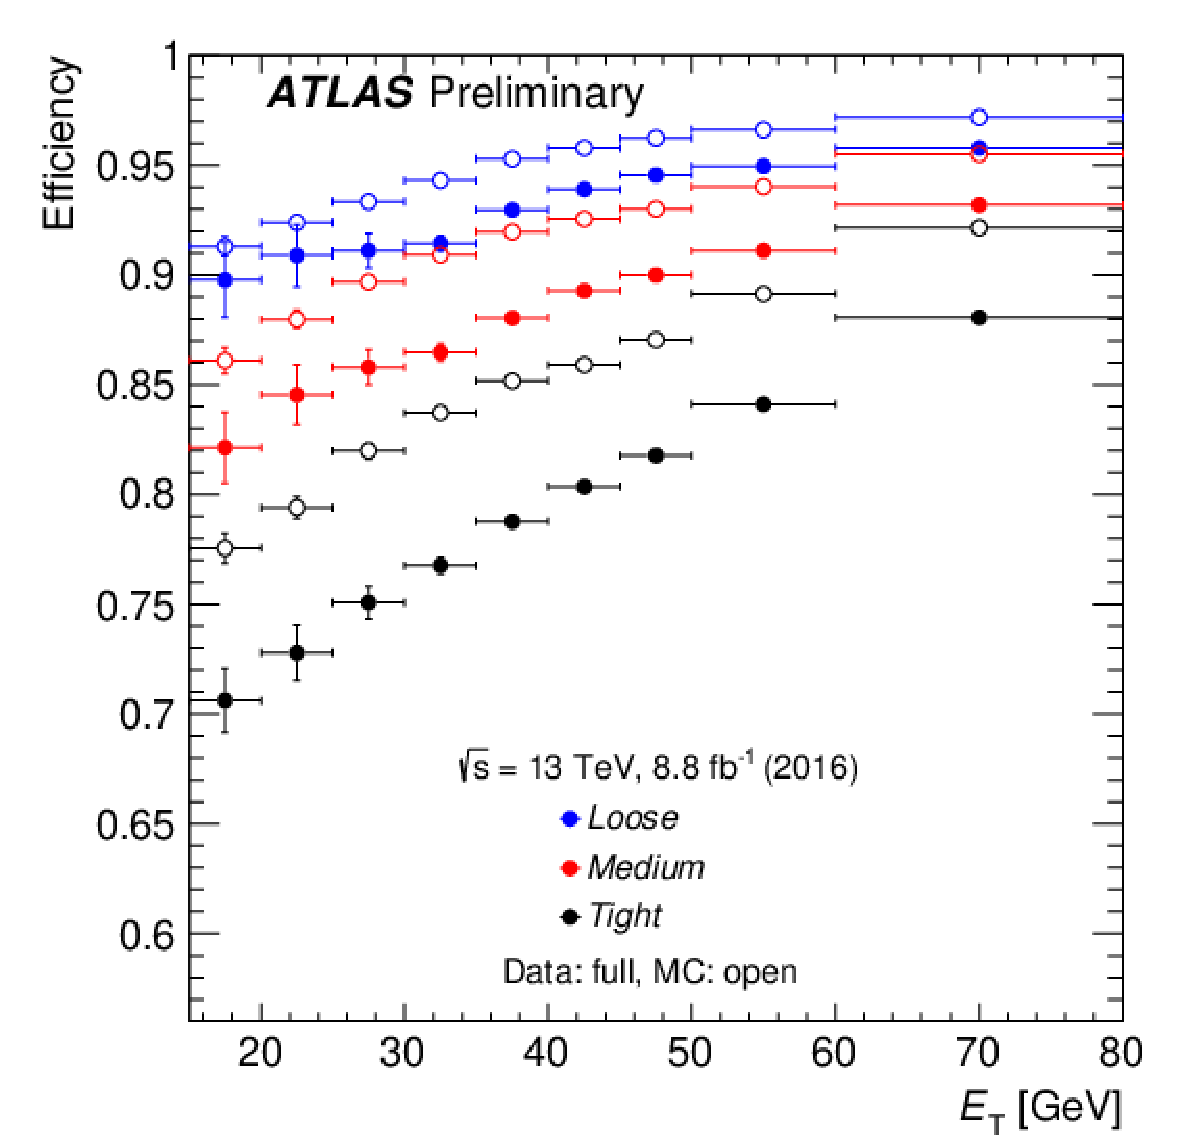
\includegraphics[width=0.4\textwidth]{figures/objects/ele_ideff_2016}  }
%\end{center}
% \caption{\subref{fig:obj:ele_sff_tight} Identification efficiency \glspl{sf} for Tight electrons in the 40-45 \et range, measured in the 2015 data. Figure from Ref. \cite{ATLAS:2016iqc}. \subref{fig:obj:ele_id2016} Electron identification efficiencies in $Z\rightarrow e e$ events. Figure from Ref. \cite{atlaselec2016}.
% }
%  \label{fig:obj:ele_sf}
%\end{figure}

The reconstruction efficiency is measured as the ratio of reconstructed electrons to the number of \gls{em} clusters. 
It is measured with a method similar to the $Z_\mathrm{mass}$ method, but with the selection criteria for the probe relaxed to include all the \gls{em} clusters. Figure \ref{fig:obj:ele_eff_pt} shows the combined reconstruction and identification efficiency in $Z\rightarrow e e$ simulated events and in the 2015 data, as a function of \et and inclusive in $\eta$.

\begin{figure}[h]
\begin{center}
  \subfigure[]{
    \label{fig:obj:ele_eff_pt}
    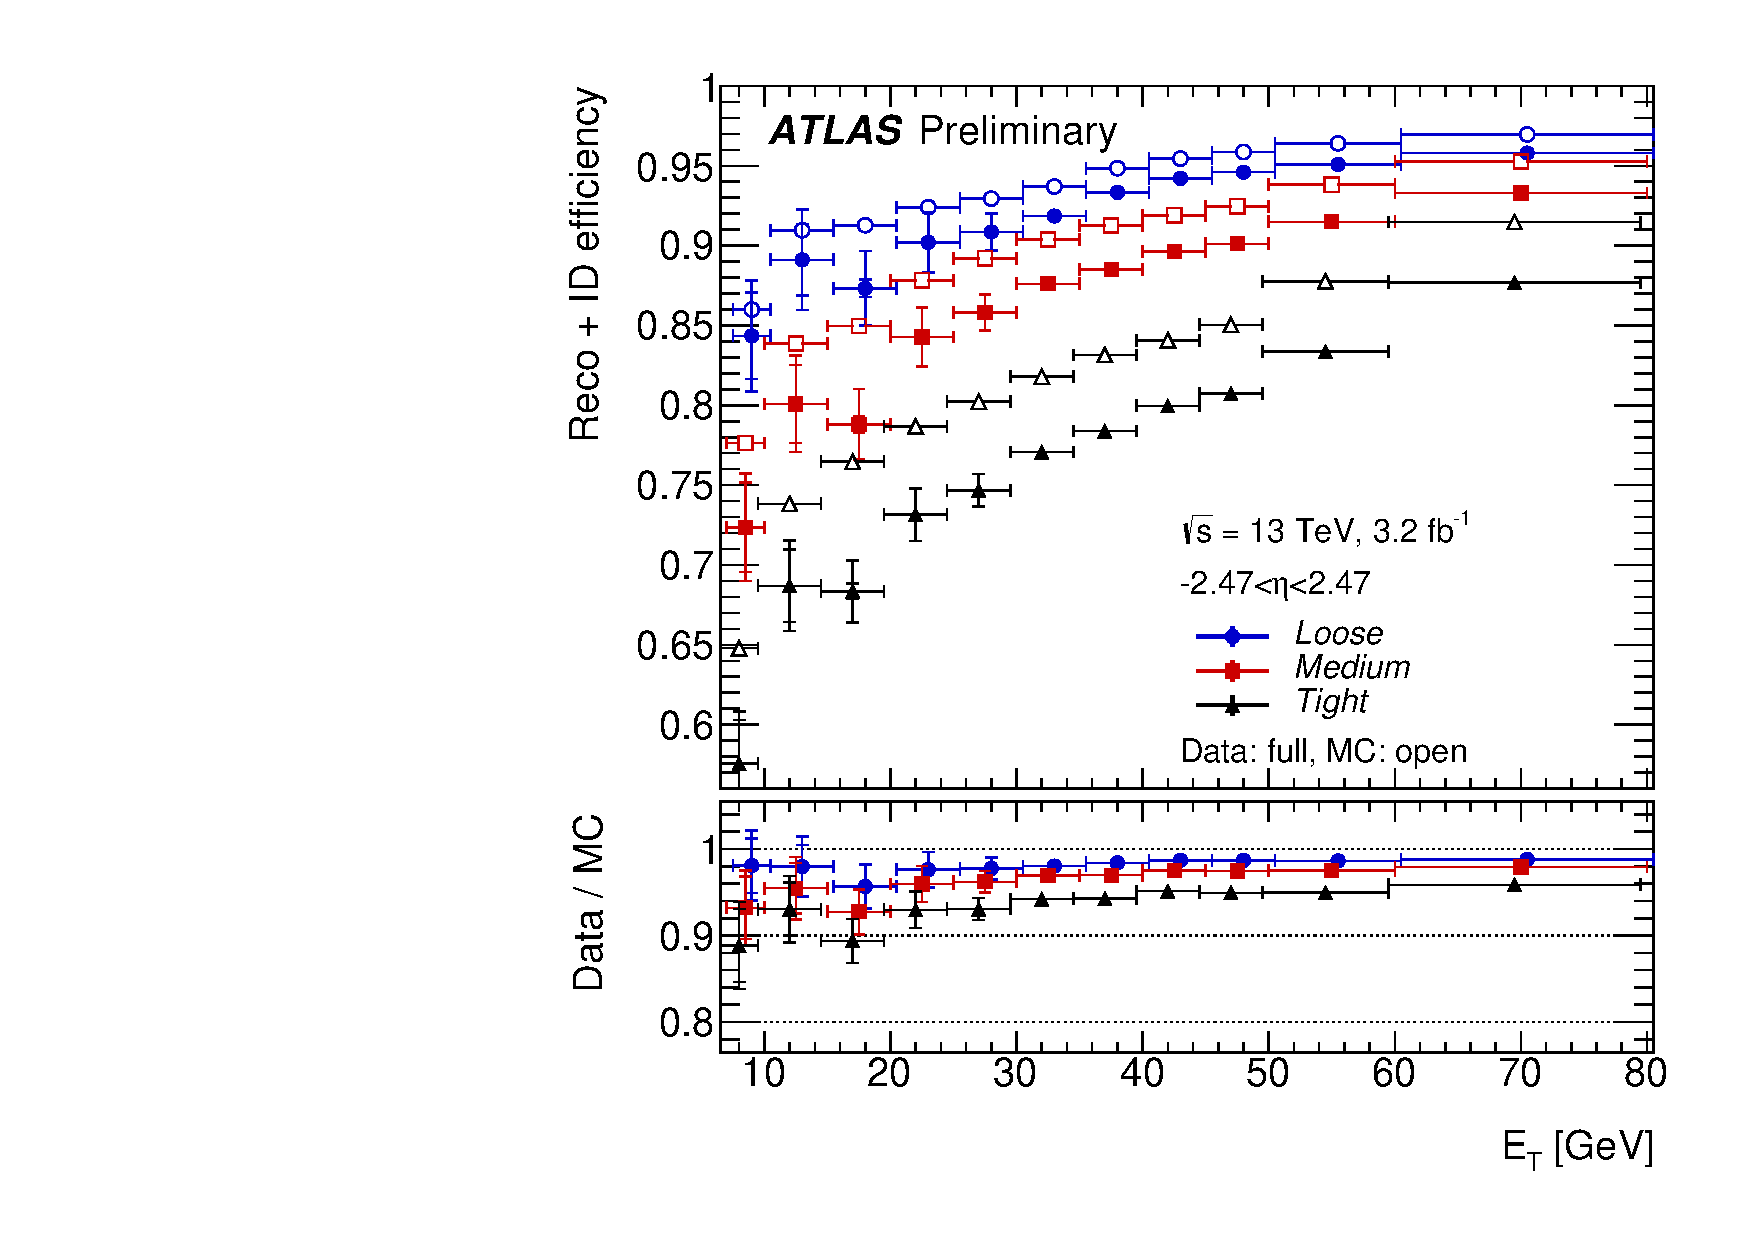
\includegraphics[width=0.4\textwidth]{figures/objects/ele_eff_pt} }
  \subfigure[]{
    \label{fig:obj:ele_eff_pt_unc}
    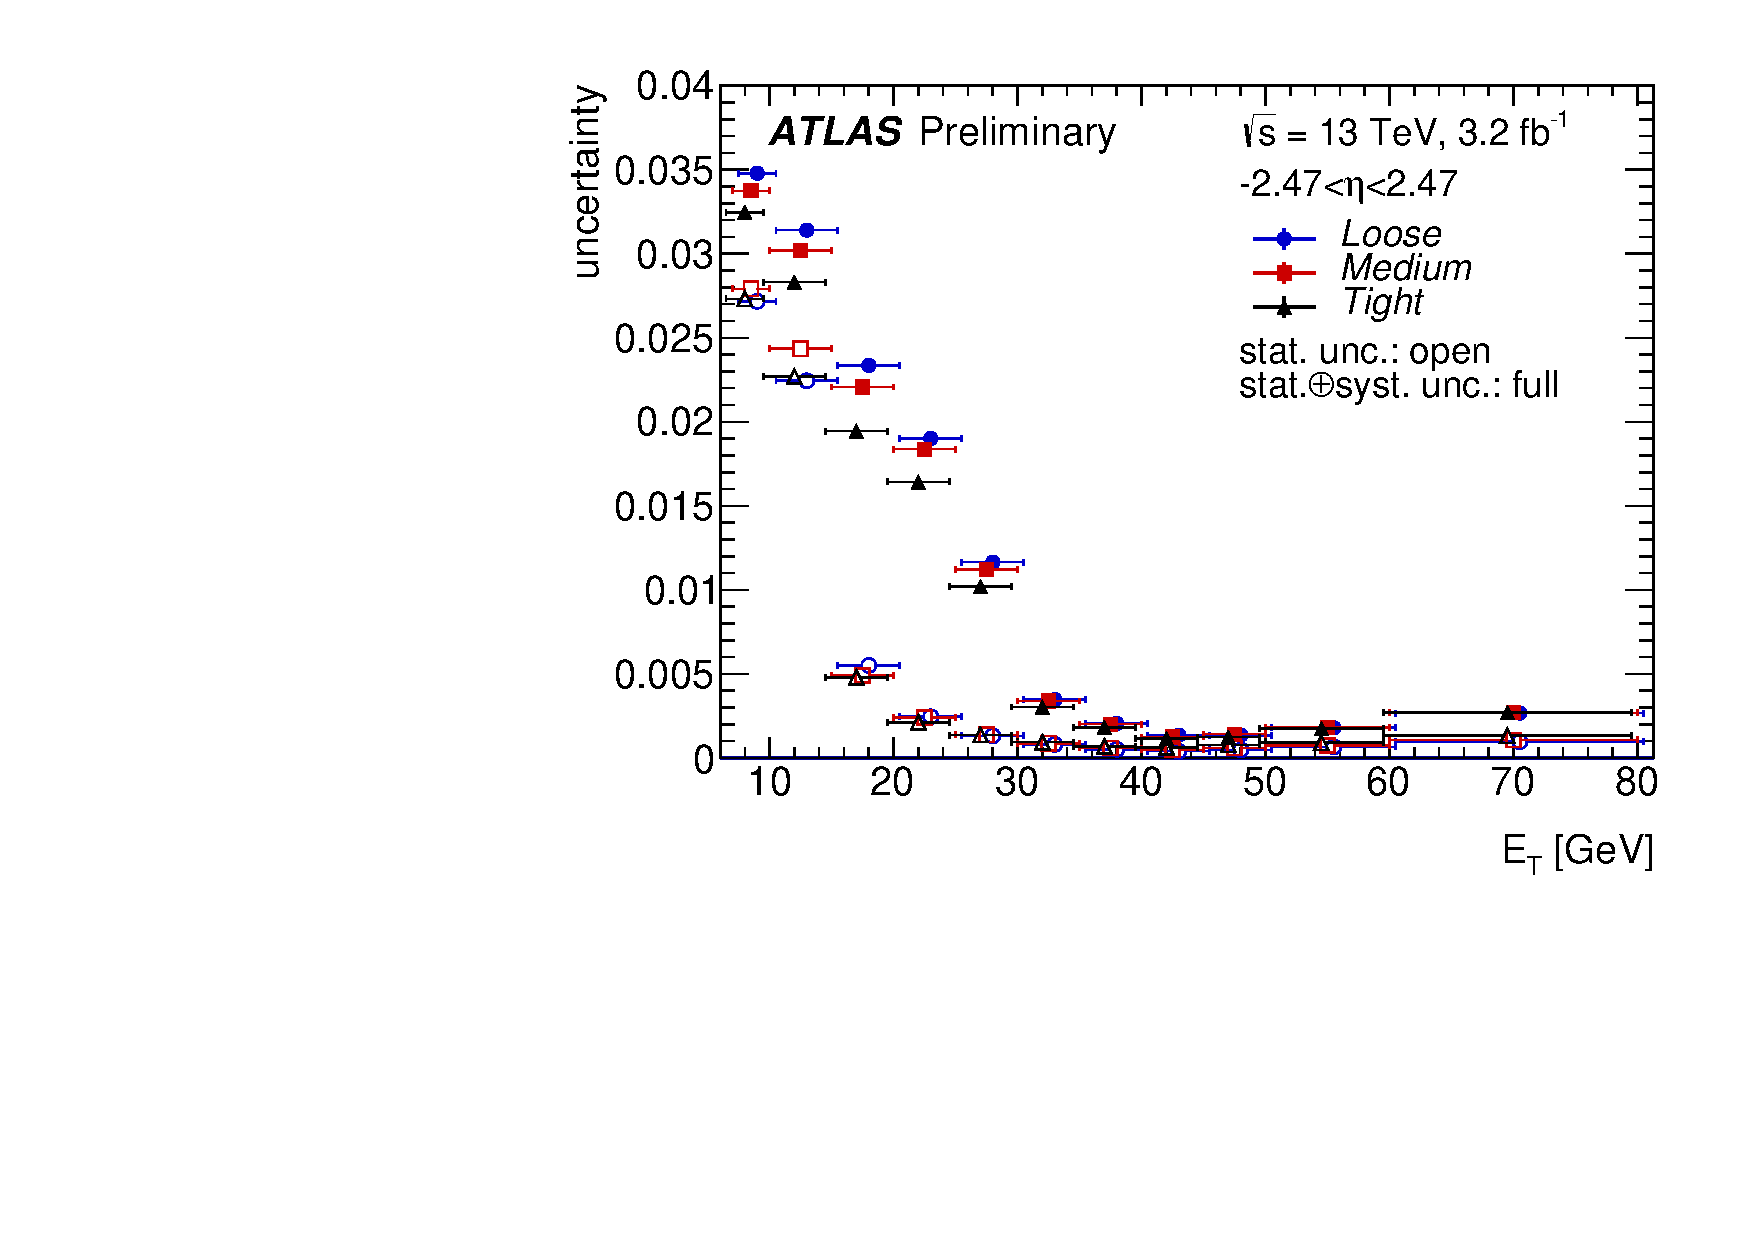
\includegraphics[width=0.5\textwidth]{figures/objects/ele_eff_pt_unc}  
    }
\end{center}
 \caption{\subref{fig:obj:ele_eff_pt} Combined electron reconstruction and identification efficiency in $Z\rightarrow e e$ simulated events and in the 2015 data and \subref{fig:obj:ele_eff_pt_unc} absolute efficiency uncertainty, as a function of \et and inclusive in $\eta$. Figures from Ref. \cite{ATLAS:2016iqc}. 
 }
  \label{fig:obj:ele_eff}
\end{figure}

Also the isolation efficiency is measured with a tag-and-probe method derived from the $Z_\mathrm{mass}$ one, but with a lower \et threshold for the 
probe electrons. For each isolation \gls{op}, the efficiency is derived with respect to each identification \gls{op}.

\subsection{Electron energy scale and resolution}
\label{sec:obj:ele_energy}

The electron energy calibration follows three steps \cite{Aad:2014nim,ATL-PHYS-PUB-2016-015}:
\begin{description}
\item[Detector response] Data-driven corrections are derived to correct for non-uniformity in the detector response, and are applied to data.
 
\item[MC-based] The energy is corrected with a \gls{bdt} that takes into account the energy deposited in front of the calorimeter (before reaching the first active layer of the calorimeter particles traverse 5-10 radiation lengths) and the changes in energy response depending on the impact point in the calorimeter.
This calibration is derived from \gls{mc} simulation and applied to both data and \gls{mc}. 

\item[In-situ] After the application of the data-driven corrections for the detector non-uniformity and of the MC-based corrections, 
residual differences in electron energy scale and resolution between data and \gls{mc} are measured with a template procedure on $Z\rightarrow e e$ events. The energy scale correction is applied to data, while a energy resolution smearing is applied to \gls{mc}.

\end{description}



\section{Missing transverse momentum}
\label{sec:met}

Particles that interact only weakly with the detector, such as neutrinos or \gls{bsm} particles like neutralinos, are not reconstructed directly.  
Their presence is instead inferred by measuring the total momentum imbalance in the event. 
The missing transverse momentum vector ($\bar{E}_{\rm{T}}^{\rm{miss}}$) is defined as the negative vector sum of the \pt of all the reconstructed calibrated objects in the event, 
plus a term that groups all the energy that is not associated to any of the reconstructed objects (soft term) \cite{Aad:2016nrq,Aaboud:2018tkc,ATLAS:2018ghb}. 
The missing transverse momentum is given by:

\begin{equation}
\bar{E}_{\rm{T}}^{\rm{miss}}=  - \sum \pt ^{e}  - \sum \pt ^{\gamma} - \sum \pt ^{\tau}    \nonumber \\
- \sum \pt ^{jets} - \sum \pt   ^{\mu} - \sum \pt  ^{soft-terms}   \;
\label{eq:etm} 
\end{equation}

\noindent The magnitude of $\bar{E}_{\rm{T}}^{\rm{miss}}$ is the missing transverse momentum (\met), and 
its azimuthal angle is $\phi^{miss}$.

The soft term includes all the detector signals that are not associated to muons, electrons, photons, taus or jets, and can receive contributions
both from the hard scattering and from pileup interactions. 
% chiara: check: in some papers it says the tracks need to pe associated to the primary vertex
In \gls{atlas} several algorithms are designed to reconstruct and calibrate the \met soft term, and the analyses discussed in this thesis use 
the one recommended for the 2015-2016 analyses, the \gls{tst}. In this algorithm, the \met soft term is reconstructed purely from track information, without any contribution from the calorimeter information; 
this results at the same time in better pileup resistance but also in the loss of information about soft neutral particles. 
An alternative version of the soft term is the \gls{cst}, that instead uses energy deposits in the calorimeters not associated to hard physics objects. 
Other algorithms are described in Ref. \cite{Aad:2016nrq}.

Three different \met \gls{op} are available, which differ in the selections on the jets that are used in the $\sum \pt ^{jets} $ term in 
Equation \ref{eq:etm} \cite{ATLAS:2018ghb}:

\begin{description}
\item[Loose] Includes all jets with $\pt>20$ GeV that pass the \gls{jvt} selection when the jet has $\pt<60$ GeV and $|\eta|<2.4$. This is the \gls{op} used in the searches presented in this thesis. 

\item[Tight] In addition to Loose criteria, the forward jets with $|\eta|>2.4$ are required to have $\pt>30$ GeV to be included in the \met computation.

\item[Forward-JVT] In addition to the Loose criteria, jets with $|\eta|>2.5$, $\pt<50$ GeV and failing the Loose fJVT criteria (described in Ref. \cite{Aaboud:2017pou}) are not included. 

\end{description}

The performance of the \met reconstruction is evaluated in data and \gls{mc} simulation, studying the mean, the width and the integral of the 
tail of the \met distribution in different topologies. 
In the 2015-2016 dataset, the \met performance has been evaluated using two different signatures. 
$Z \rightarrow \ell \ell$ events are studies both \gls{mc} simulation and in data, since the leptonic decay of the $Z$ boson are 
abundant and easy to trigger. 
These events do not contain any real \met, therefore all the reconstructed \met can be assigned to mismeasurement effects. 
The second signature used is vector boson fusion $h \rightarrow WW$ events, where both $W$ bosons decay to 
a lepton and a neutrino; this topology is studied in \gls{mc} simulation only. 

The comparison of the \met distribution with the Loose \gls{op} and of the \met soft term in data and simulation is shown in Figure 
\ref{fig:obj:met_fig_7a} and \ref{fig:obj:met_fig_7b} respectively, in a $Z \rightarrow ee$ event selection.

\begin{figure}[htbp]
\begin{center}
  \subfigure[]{
    \label{fig:obj:met_fig_7a}
    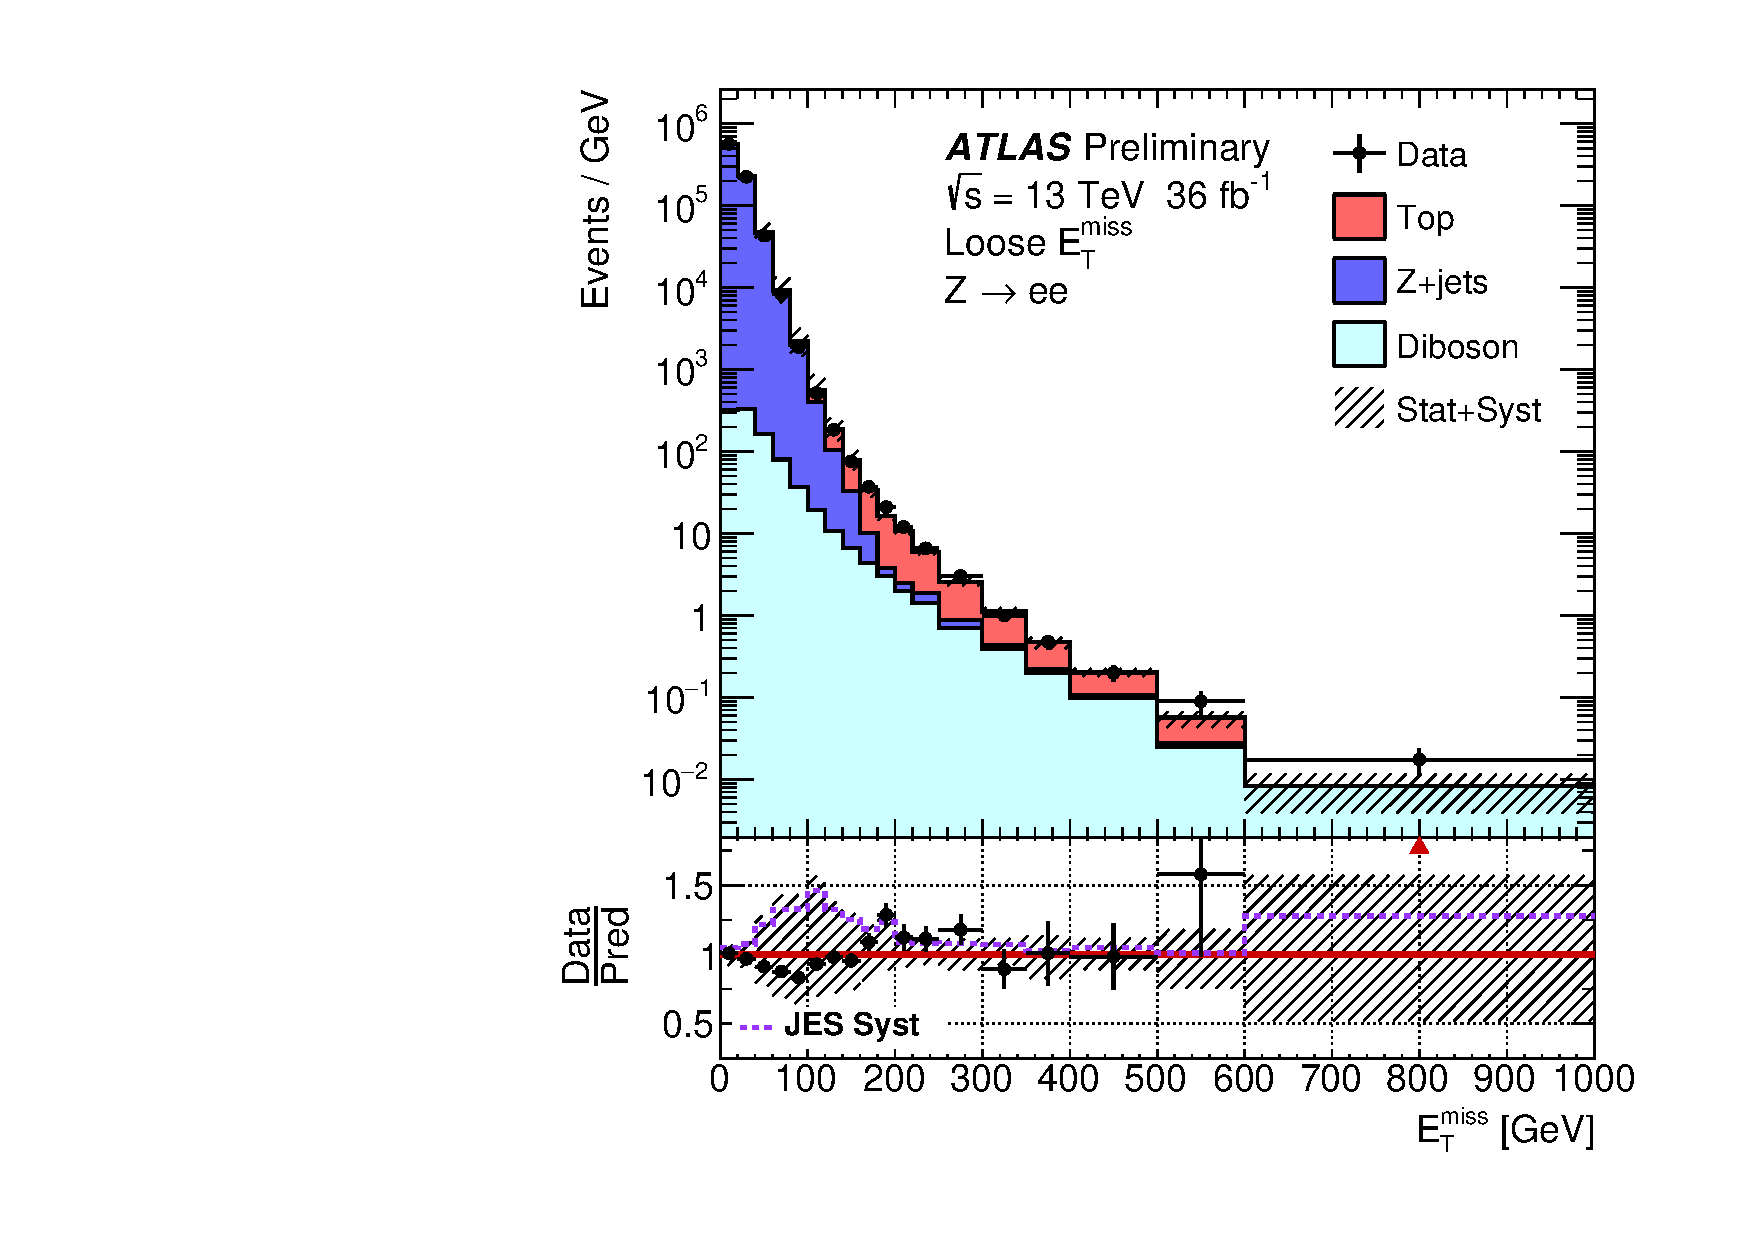
\includegraphics[width=0.48\textwidth]{figures/objects/met_fig_07a.pdf} }
  \subfigure[]{
    \label{fig:obj:met_fig_7b}
    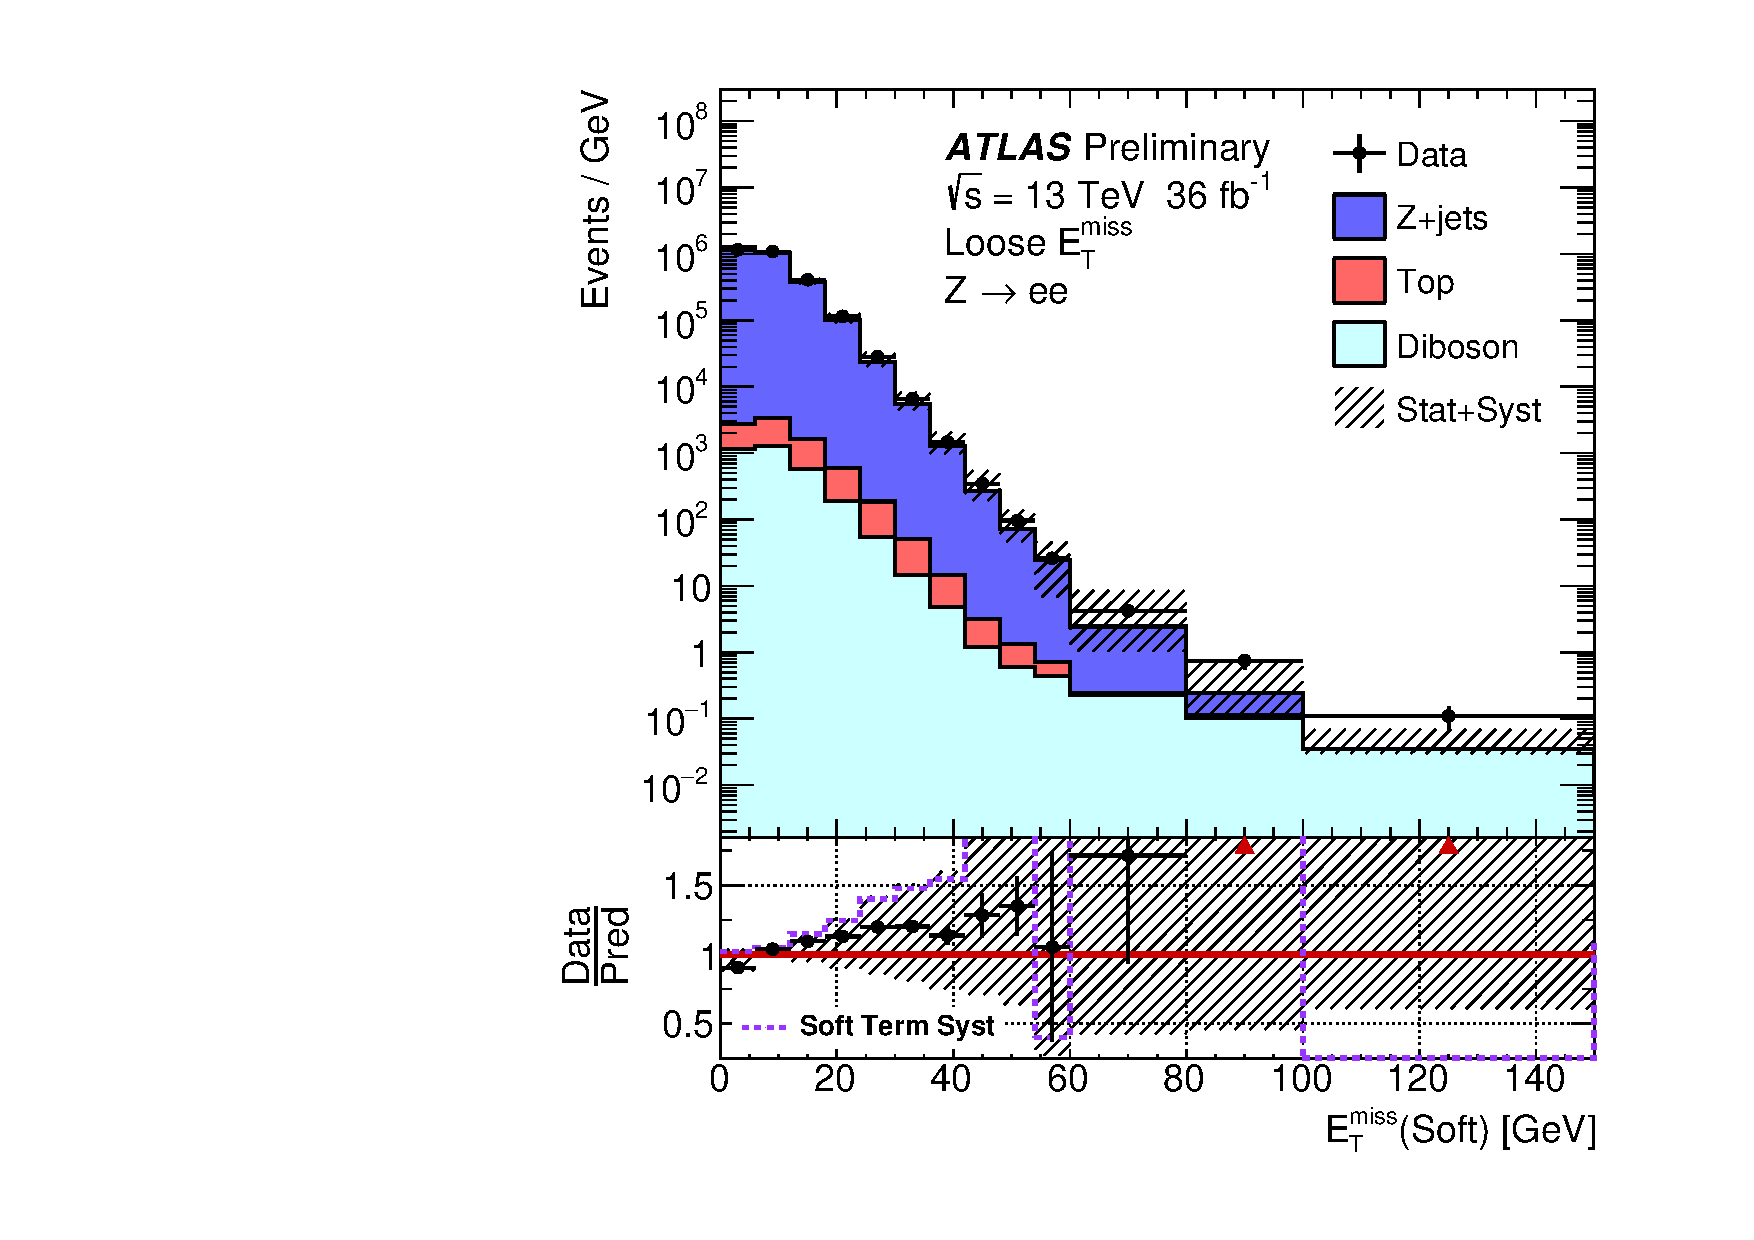
\includegraphics[width=0.48\textwidth]{figures/objects/met_fig_09a.pdf}  
    }
\end{center}
 \caption{
 Distribution of \subref{fig:obj:met_fig_7a}  \met using the Loose \met \gls{op} in data and simulation 
 and \subref{fig:obj:met_fig_7b} \met soft term  in a $Z \rightarrow ee$ event selection. 
Figures from Ref. \cite{ATLAS:2018ghb}. 
 }
  \label{fig:obj:met_fig_7}
\end{figure}


The \met resolution, defined as the \gls{rms} obtained from the combined distribution of the 
$x$ and $y$ components, respectively $E_x^{\rm{miss}}$ and $E_y^{\rm{miss}}$, is shown in Figure \ref{fig:obj:met_fig_11} for 
the Loose \gls{op}. 
The simulation agrees well with data within the uncertainties.
In the definition of the resolution, the \gls{rms} is preferred over the width of a Gaussian fit to the distribution  
to preserve the information on the tail. 
The systematic uncertainties on the energy scale and resolution of all the physics objects are propagated to the \met computation.
The only systematic uncertainties affecting only \met are the ones related to the soft term, which are measured 
$Z \rightarrow \ell \ell$ events by comparing the simulation with data.



\begin{figure}[htbp]
\begin{center}
  \subfigure[]{
    \label{fig:obj:met_fig_11a}
    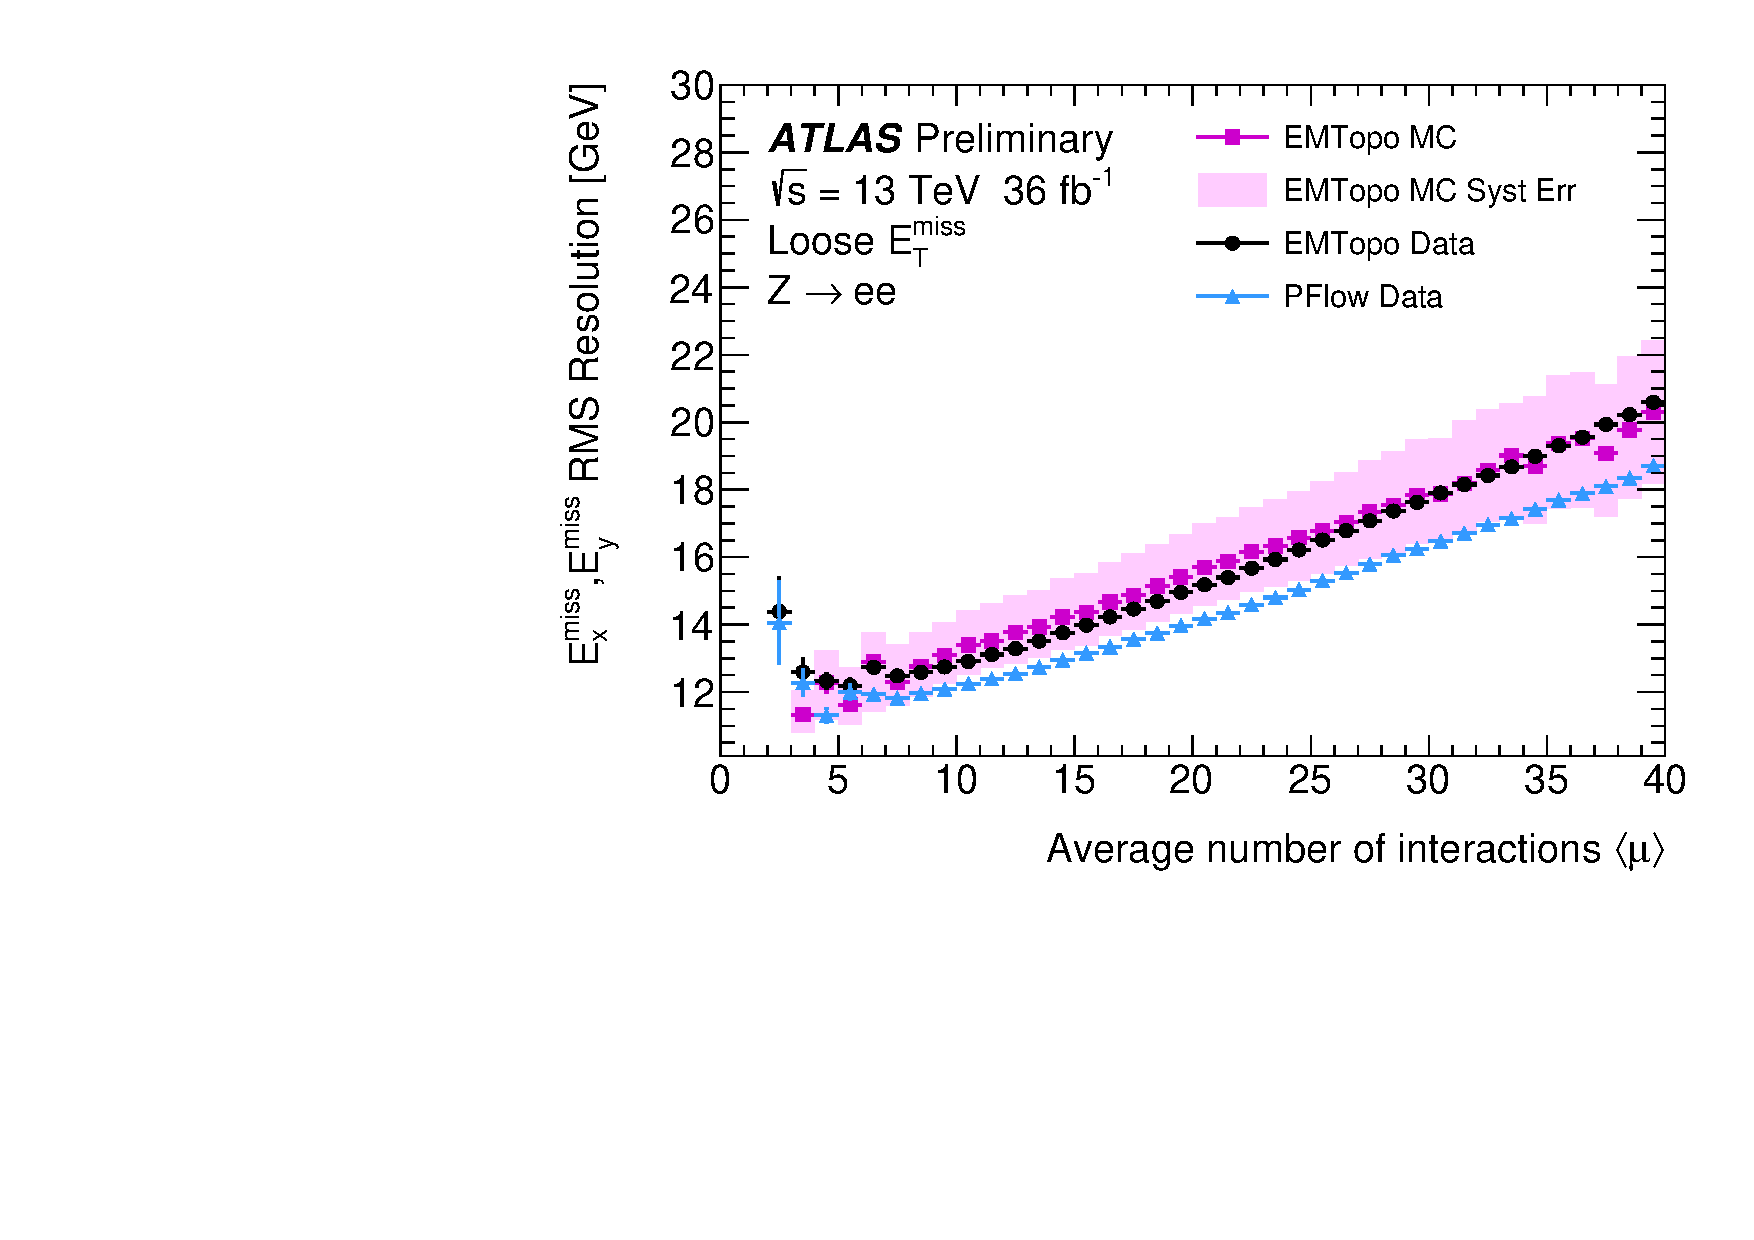
\includegraphics[width=0.48\textwidth]{figures/objects/met_fig_11a} }
  \subfigure[]{
    \label{fig:obj:met_fig_11b}
    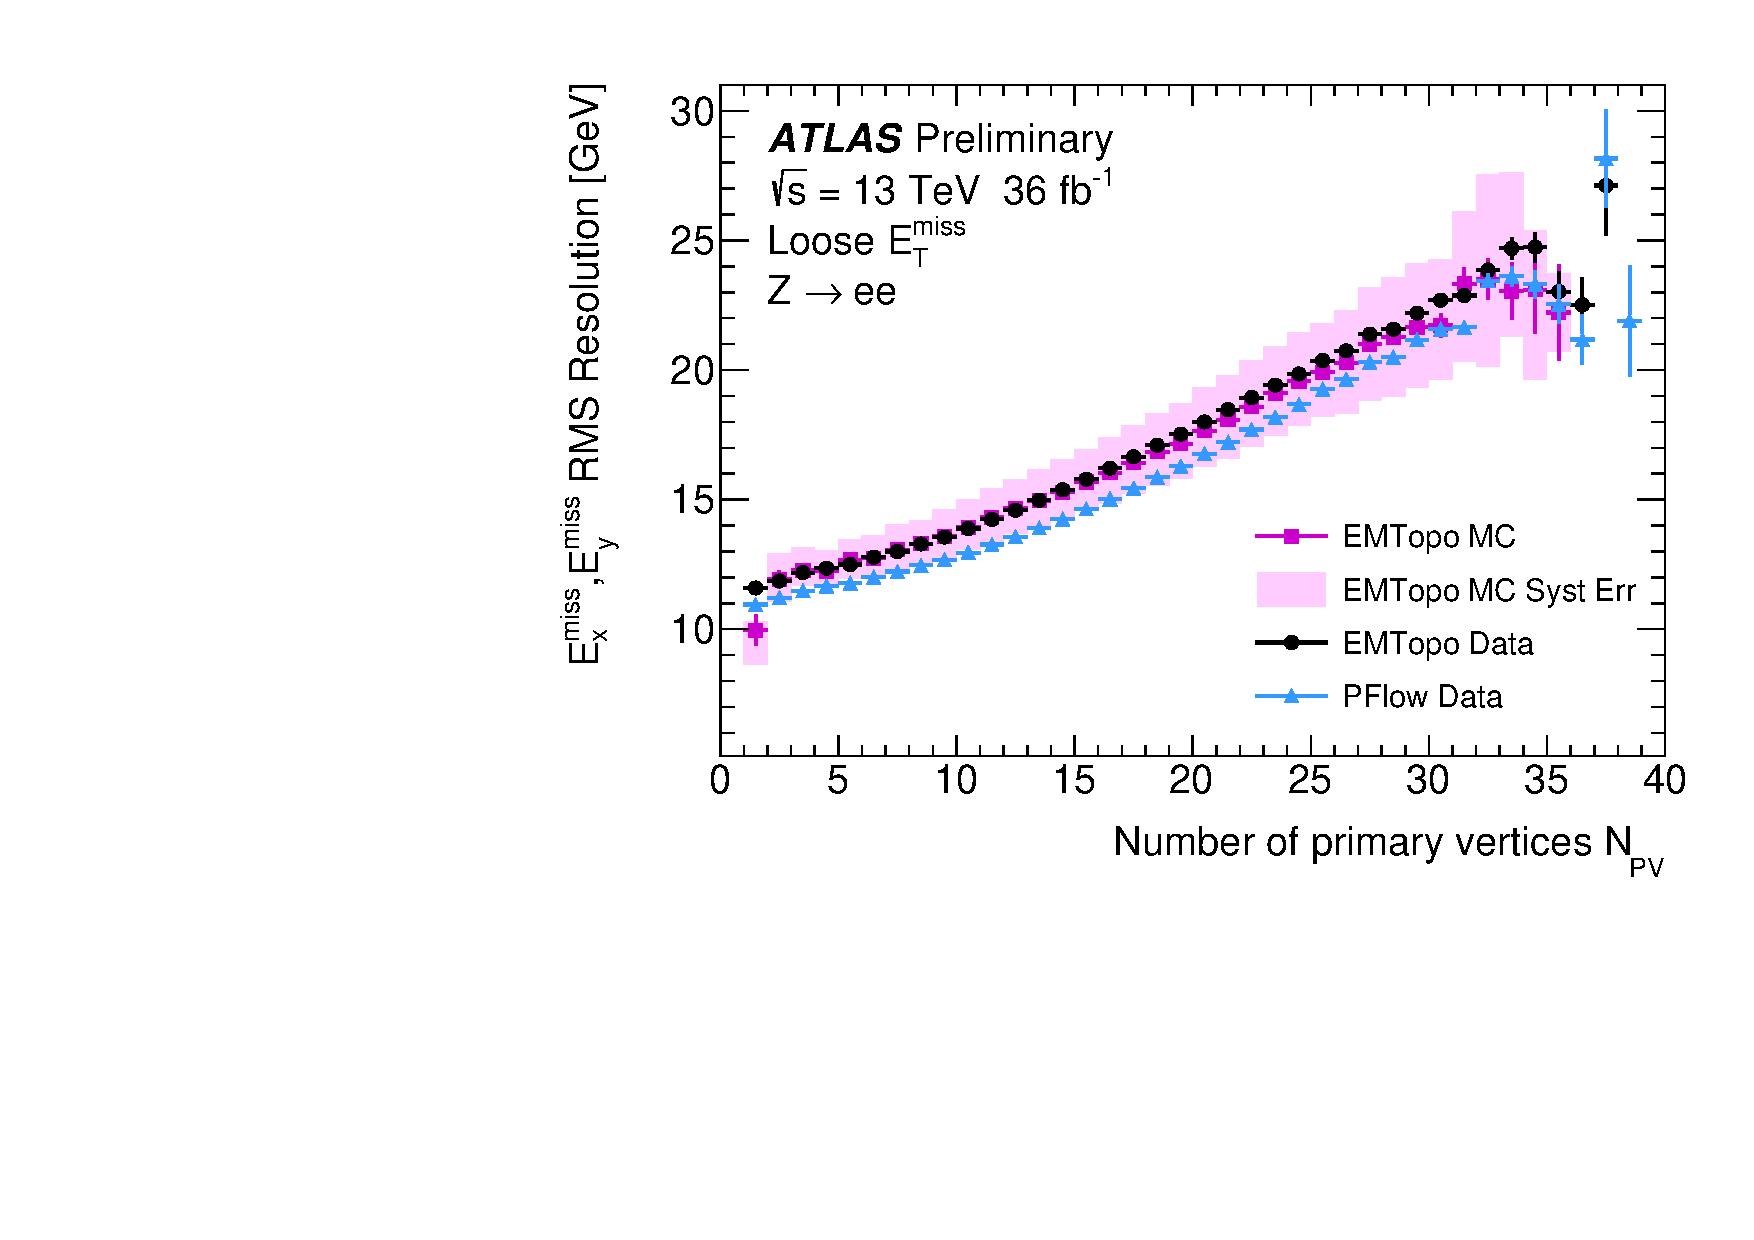
\includegraphics[width=0.48\textwidth]{figures/objects/met_fig_11b}  
    }
\end{center}
 \caption{
 The \gls{rms} obtained from the combined distributions of \met using the Loose \met \gls{op} 
 for data with EMTopo jets (circular marker) and PFlow jets (triangular marker) and \gls{mc} simulation
with EMTopo jets (square marker) in a $Z \rightarrow ee$ event selection are shown versus \subref{fig:obj:met_fig_11a} $<\mu>$ and 
\subref{fig:obj:met_fig_11b} number of primary vertices. 
Figures from Ref. \cite{ATLAS:2018ghb}. 
 }
  \label{fig:obj:met_fig_11}
\end{figure}



 
